\documentclass[16pt]{report}
\usepackage[utf8]{vntex, inputenc} % vntex first to avoid Vietnamese auto captions
\usepackage[english]{babel}
\usepackage{suthesis-ug}
\usepackage{algorithm2e}
\usepackage{amsmath}
\usepackage{booktabs}
\usepackage{authblk}
\usepackage[labelfont=bf]{caption}
\usepackage{cases}
\usepackage{color}
\usepackage{graphicx}
\usepackage[unicode]{hyperref}
\usepackage{multirow}
\usepackage{subcaption}
\usepackage{biblatex}
\usepackage{tabularray}
\usepackage{xcolor}
\hypersetup{
    colorlinks=true,
    linkcolor=black,
    filecolor=magenta,      
    urlcolor=black,
    pdftitle={Overleaf Example},
    pdfpagemode=FullScreen,
    citecolor=black,
    }
\urlstyle{same}
% Global layout
\usepackage{fancyhdr, graphicx, hyperref, indentfirst, lastpage, setspace, titlesec, enumitem}
\usepackage[top=3.5cm, bottom=3.0cm, left=3.5cm, right=2.0cm]{geometry} % căn lề theo quy chuẩn KLTN
% Encodings
\usepackage{amsmath, amsthm, amssymb, gensymb}

% Better table
\usepackage{array, booktabs, multicol, multirow, siunitx}
\usepackage{caption, float}
\restylefloat{table} % The table does not float anymore
% Code space
% \usepackage[dvipsnames]{xcolor}
\usepackage[framemethod=tikz]{mdframed}
\usepackage{minted} % needs --shell-escape flag
\usepackage{listings} % to format code
\usepackage{tikz}
\pagestyle{fancy}
\usepackage{array}
\usepackage{longtable}
\RestyleAlgo{ruled}
\newtheorem{theorem}{Theorem}
\newtheorem{definition}{Definition}

\def\checkmark{\tikz\fill[scale=0.4](0,.35) -- (.25,0) -- (1,.7) -- (.25,.15) -- cycle;} 
\setcounter{secnumdepth}{3}

\usepackage{xcolor}

\definecolor{codegreen}{rgb}{0,0.6,0}
\definecolor{codegray}{rgb}{0.5,0.5,0.5}
\definecolor{codepurple}{rgb}{0.58,0,0.82}
\definecolor{backcolour}{rgb}{0.9,0.9,0.9}

\lstdefinestyle{mystyle}{
    backgroundcolor=\color{backcolour},   
    commentstyle=\color{codegreen},
    keywordstyle=\color{magenta},
    numberstyle=\tiny\color{codegray},
    stringstyle=\color{codepurple},
    basicstyle=\ttfamily\footnotesize,
    breakatwhitespace=false,         
    breaklines=true,                 
    captionpos=b,                    
    keepspaces=true,                 
    numbers=left,                    
    numbersep=5pt,                  
    showspaces=false,                
    showstringspaces=false,
    showtabs=false,                  
    tabsize=2
}


\lstset{style=mystyle}


\addbibresource{references.bib}
\begin{document}
\setstretch{1.25}
\setlength{\parindent}{0pt}




\begin{titlepage}
\begin{center}
\textbf{\fontsize{13pt}{18pt}\selectfont VIETNAM NATIONAL UNIVERSITY}\\
\textbf{\fontsize{13pt}{18pt}\selectfont HO CHI MINH CITY UNIVERSITY OF TECHNOLOGY}\\
\textbf{\fontsize{13pt}{18pt}\selectfont FACULTY OF COMPUTER SCIENCE AND ENGINEERING}
\end{center}

\vspace{1cm}

\begin{center}
\begin{tabular}{c}
{\fontsize{13pt}{18pt}\selectfont - SPECIALIZED PROJECT- }\\
~~\\
\hline
\\
% \multicolumn{1}{l}{\textbf{{\Large Assignment}}}\\
\\
\textbf{{\huge Develop application to help students}}\\
\textbf{{\huge search for rentals }}\\
\\
\\
\hline
\end{tabular}
\end{center}

\vspace{1cm}

\begin{figure}[h!]
\begin{center}

\includegraphics[width=6cm]{Images/BK.png}
\end{center}
\end{figure}



\vspace{1cm}


\begin{table}[h]
\begin{tabular}{rll}
\hspace{3 cm}
& Thesis Committee: &Computer Science CS-CC 12\\
& Supervisor: &Assoc. Prof. Phạm Trần Vũ, PhD\\
& Reviewer: &M.S. Nguyễn Mạnh Thìn \\
& Students: & Nguyễn Công Đạt - 2052942. \\
& & Nguyễn Trần Minh Phước - 2052662\\
\end{tabular}
\end{table}


\begin{center}
{\footnotesize HO CHI MINH CITY, November 2023}
\end{center}
\end{titlepage}



\prefacesection{Declaration of Authenticity}
We certify that the research described in the following sections was carried out by us under the direction and supervision of Associate Professor Dr. Pham Tran Vu. The outcome of our research is reliable and hasn't been released in any other format previously. The references section includes a complete list of all the sources from which the research's materials were gathered.

We also utilized the findings of several other authors and organizations in our study. All of them have been appropriately cited.

We stand by our conduct and will take responsibility for any instances of plagiarism. Therefore, the University of Technology - Vietnam National University HCMC disclaims all liability for any copyright violations committed during our study.

\begin{flushright}
\begin{tabular}{c}
    Ho Chi Minh City, December 2023\\
    Authors\\
\end{tabular}
\vspace{1cm}
\end{flushright}
\begin{flushright}
\begin{tabular}{cc}
    Nguyen Tran Minh Phuoc & Nguyen Cong Dat
\end{tabular}
\end{flushright}
\prefacesection{Acknowledgements}
We would like to acknowledge and give our deepest gratitude to everyone who has supported us throughout the project.

\hfill

To begin with, we want to give our sincere appreciation to our supervisor, Associate Professor Dr. Pham Tran Vu for his guidance and support. His guidance and support have helped us to complete the project.

\hfill

Next, we would like to thank Luu Chan Hung - the Bach Khoa alumni for his valuable advice and support. He helps us to improve the project and also shares advice on how to write a better report. 

\hfill

Finally, we want to thank our family and all of our friends who have supported us in the project.
\prefacesection{Abstract}
To solve the difficulty in finding the accommodations, we developed a system that allows the landlord to post their rental information and users to search for their desired rental. Besides that, we also have a crawler service to collect rental data from different sources such as Facebook and some popular real estate websites to enrich our rental data. Then we build a chatbot to help students search for the rental information.

\noindent Our main focus is on web development technology, data crawling techniques and how to apply the machine learning model in the Natural Language Processing field, especially in the Intent Classification and Name Entity Recognition task.
\afterpreface

\chapter{Introduction}

\section{Motivation}
Currently, rental room listings are posted on various sources such as real estate websites or Facebook groups. This makes the process of finding accommodations more challenging. Users often have to spend many hours on different websites to find a suitable room. Moreover, some sources for room listings lack the functionality to search according to users' needs. For example, in case of the rental posts on Facebook groups, users face a limitation in searching for posts based on crucial criteria such as price, location, or area,... Therefore, recognizing the problem, we want to build a system that centralizes all the rental posts in different sources and also provides an interactive way to search for posts based on users' preferences.

\section{Current solutions}
In this section, we will discuss some related works that are relevant to our thesis and represent the advantages and disadvantages of them.

\subsection{Facebook pages and groups}
Facebook is the most popular social network in the work. Therefore, Facebook pages and groups also become popular platforms for people to post their rental listings, as well as find accommodations. With the keyword "phòng trọ" you can see there are a lot of groups/pages with more than 100.000 members and >10 posts per day in Figure \ref{fig:facebook-group}

\begin{figure}[ht]
    \centering
    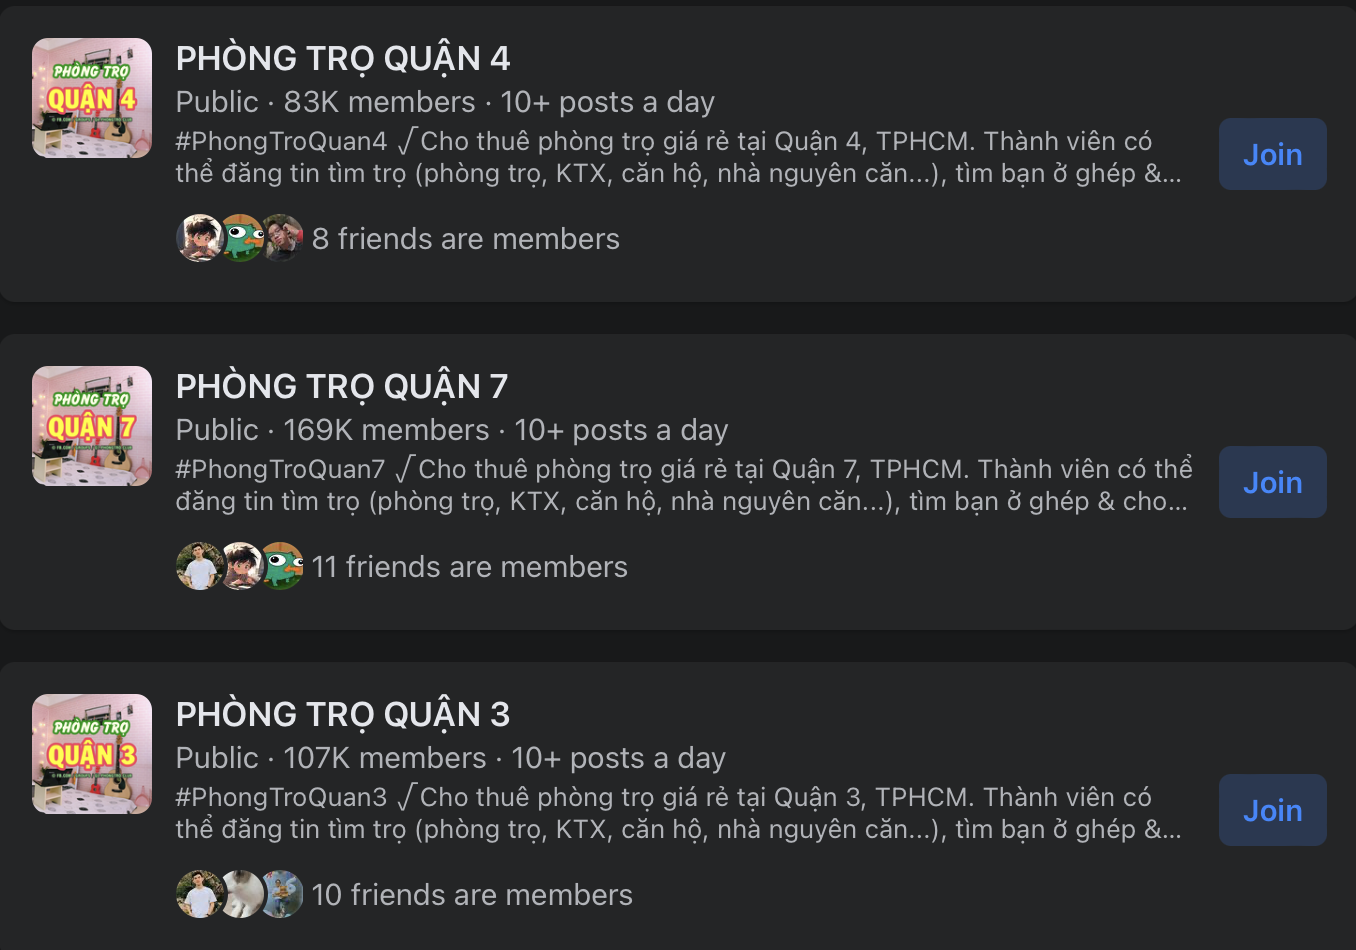
\includegraphics[width=0.8\textwidth]{images/1.Introduction/facebook_groups.png}
    \caption{The list of Facebook groups with the keyword "phòng trọ"}
    \label{fig:facebook-group}
\end{figure}

\noindent So Facebook is a good source for users to find accommodations. However, there are some disadvantages when using Facebook to find accommodations:
\begin{itemize}
    \item \textbf{The data is distributed in groups/pages}: There are many groups/pages for rental listings on Facebook. Therefore, users have to spend a lot of time with each group and find suitable accommodations.
    \item \textbf{Lack of search functionality}: Facebook does not provide a search functionality for users to search for posts based on their preferences. Therefore, users have to scroll through the posts to find the suitable ones.
\end{itemize}

\subsection{Real estate websites}
In the real estate market, many websites provide rental listings. Some of the most popular websites are nhattot.vn, batdongsan.com.vn, mogi.vn,... These websites provide a search functionality for users to search for rental listings based on their preferences. However, these websites do not have much data compared to Facebook groups/pages. Therefore, users have fewer choices when using these websites. One reason for that is the process of posting a rental listing on these websites is more complicated than on Facebook. Moreover, these websites provide different interfaces for users to interact with. Therefore, users have to get used to the user interface of each website. This makes the process of finding accommodations more challenging.

\section{Goal}
Understanding the problem of current websites in the market, we aim to provide a new solution that helps users find accommodations more easily. Our goal is to build an application that collects rental data from both Facebook groups/pages and real estate websites and provides a unified user interface. So instead of jumping between different websites, users can use our application to search for rental posts from different sources in one place. Moreover, our system also provides a chatbot interface to help users search for rental posts based on their preferences naturally and interactively. The feature list is shown below
\begin{itemize}
    \item Develop a crawler to collect rental data from Facebook groups, pages and other popular websites for finding accommodations in Vietnam such as nhattot.vn, batdongsan.com.vn.
    \item The data crawled from Facebook groups and pages is in the unstructured format. Therefore, we need to develop a Machine Reading comprehension model to extract the structured data from the unstructured data.
    \item Develop a website to display rental posts and allow the landlords to post their rooms for rent.
    \item Build the conversational chatbot that supports searching for rental posts based on users' preferences.
\end{itemize}

\section{Scope}
In the scope of this project, we mainly focus on the following tasks:

\begin{itemize}
    \item \textbf{Crawler}: we develop a crawler first, to collect the data from different sources. The data is also used to train the Machine Reading comprehension model.
    \item \textbf{Intent classification}: we build a modal to classify the user's intent based on the user's message.
    \item \textbf{Named Entity Recognition}: we build a model to extract the entities from both the user's message and the rental posts on Facebook pages. We want to get the structured data from the unstructured text.
    \item \textbf{Rental Website}: a website allows landlords to post their room for rent and users to search for accommodations.
    \item \textbf{Chatbot}: we built a chatbot to help users search for rental posts based on their preferences.
\end{itemize}

\chapter{Theoretical Background}
\label{chap:theoretical-background}

\section{Natural Language Processing}
Natural Language Processing is the field of Artificial Intelligence that gives the computers ability to understand text and spoken words in the same way human beings can. Natural Language Processing is a very broad field, it includes many sub-fields, such as text classification, name entity recognition, machine translation, etc. In this thesis, we focus on text classification and name entity recognition.

\section{Intent Classification}

Intent classification is the text classification task that aims to classify the user's input into a predefined set of intents. For example, in the case of a rental house search, the user's input "I want to rent a house in Ho Chi Minh City" is classified into the "rent\_house" intent.

There are two main approaches to intent classification: rule-based and machine learning-based. The rule-based approach uses a set of rules to classify the user's input. For example, the rule "if the user's input contains the word 'rent' and the word 'house', then the intent for this sentence is 'rent\_house'". One major drawback of the rule-based approach is that it requires a lot of effort and domain knowledge to create these rules.


The machine learning-based approach uses machine learning algorithms to learn the mapping between the user's input and the intent. Intent classification is a supervised learning problem, so the machine learning algorithm needs to be trained on the dataset of the user's input and the corresponding intent. The machine learning-based approach is more flexible than the rule-based approach because it does not require domain knowledge to create the rules. However, it requires a large amount of data to train the machine learning algorithm.

\section{Name Entity Recognition (NER)}
Name Entity Recognition is the task that determines the entities in the user's input. Figure \ref{fig:ner_example} illustrates an example of NER. In this example, we have 3 entities: "Sebastian Thrun" (Person), "Google" (Organization), and "2007" (Date).

\begin{figure}[ht]
    \centering
    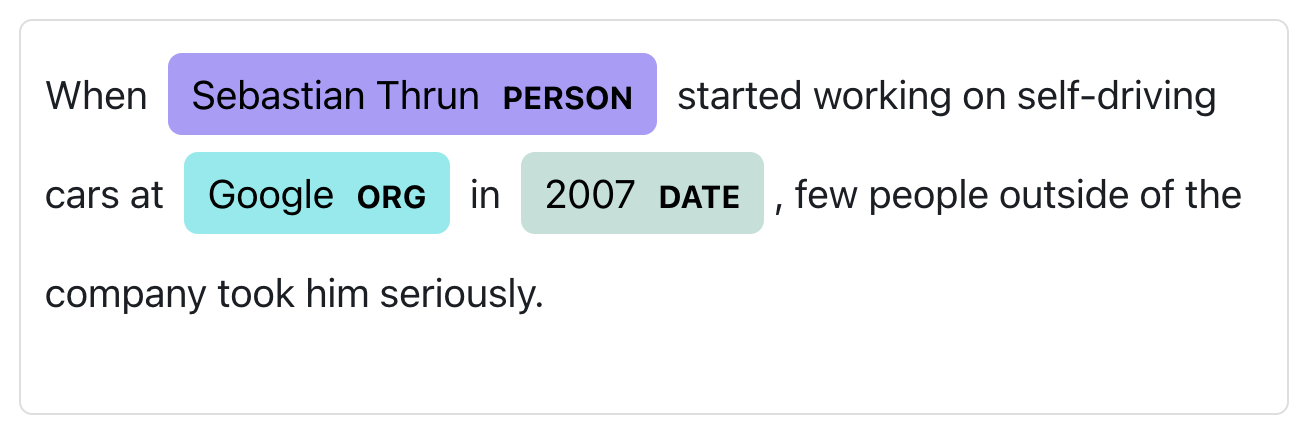
\includegraphics[width=0.8\textwidth]{Images/5.Theoretical_Background/ner_example.png}
    \caption{Example of NER, from \cite{spacy-visualizer-doc}}
    \label{fig:ner_example}
\end{figure}


To train the model for NER, we need to annotate the entities in the dataset. The popular format for annotating is BIO. In the BIO annotation, each word in the user's input is annotated with one of three labels: B, I, or O. The B label indicates the beginning of an entity, the I label indicates the inside of an entity, and the O label indicates that the word is not an entity. For example, the user's input "I want to rent a house in Ho Chi Minh City." is annotated as follows (Table \ref{tab:bio_annotation})

\begin{table}[ht]
    \centering
    \begin{tabular}{|c|c|c|c|c|c|c|c|c|c|c|}
        \hline
        I & want & to & rent & a & house & in & Ho & Chi & Minh & city \\    
        \hline
        O & O    & O  & B-TRAN & O & B-TYPE & O  & B-LOC    & I-LOC & I-LOC & I-LOC \\
        \hline
    \end{tabular}
    \caption{Example of BIO annotation}
    \label{tab:bio_annotation}
\end{table}

\section{Language Model}
A language model is a model that can determine the probability of the sequences of words. A language model is trained on a large dataset of text to predict the next word in the given context. The training process aims to enable the model to learn the patterns, structures, and relationships present in that language. 

There are two main types of language models: statistical-based models and neural network-based models. One of the most popular pure statistical language models is the n-grams model. These models are based on the consumption that the probability of the next word depends only on the previous n-1 words. However, these models have some drawbacks such as the inability to capture the long-term dependencies between the words. For that reason, the neural network language models are introduced and have become state-of-the-art in NLP. The neural network language models can understand complex patterns and capture the contextual information of the words.

\section{Word Representation}
Neural networks and deep learning can only take the numerical values as the input, so we need to convert the words into the numerical values. So in natural language processing, we need a way to represent the words as the numerical values. There are many techniques for word representation, such as One-hot representation, Bag of Words, TF-IDF, Word2Vec, etc. 

\subsection{One-hot representation}
To understand the one-hot representation, we need to understand the concept of vocabulary. The vocabulary is the set of all words in the corpus. For example, consider the corpus contains 2 sentences: "I want to rent a house in Ho Chi Minh City" and "I want to lease a room in District 1". The vocabulary of this corpus is \{"I", "want", "to", "rent", "a", "house", "in", "Ho", "Chi", "Minh", "city", "lease", "room", "district", "1"\}.

One-hot representation is the technique of converting the words into the one-hot vectors. The one-hot vector is the vector that has a length equal to the number of words in the vocabulary. The one-hot vector has a value of 1 at the index of the word in the vocabulary, and a value of 0 at the other indices. Consider the example vocabulary above, the one-hot vector of the word "rent" is [0, 0, 0, 1, 0, 0, 0, 0, 0, 0, 0, 0, 0, 0, 0]. Because the word "rent" is at the index 3 in the vocabulary, so the one-hot vector has the value of 1 at the index 3, and the value of 0 at the other indices.

\noindent The one-hot representation is very simple, but it has some drawbacks. 
\begin{itemize}
    \item The one-hot representation does not preserve the semantic relationships of the words. We want words that have similar meanings to also have similar representations.
    \item The one-hot representation is a sparse vector (the vector has only 1 non-zero value). The problem is that it requires a high-dimensional vector to represent the words, so training becomes slower and more complex. For example, we have 10000 words in the vocabulary, so we need a vector with a length of 10000 to represent each word.
\end{itemize}

\subsection{Word Embedding}
Word Embedding appears to solve the limitations of some traditional methods like one-hot encoding or Bag of Words. Word embedding is the technique that converts words into dense vectors in a low-dimensional vector space, preserving the semantic relationships of the words.

Figure \ref{fig:word_embedding} illustrates an example of Word Embedding representation in 2D space. In this example, the words in the same topics are close to each other. As a result, we have clusters for words in other topics, such as city, food, travel, etc. This example shows that Word Embedding can preserve the semantic meaning of the words.

\begin{figure}[ht]
    \centering
    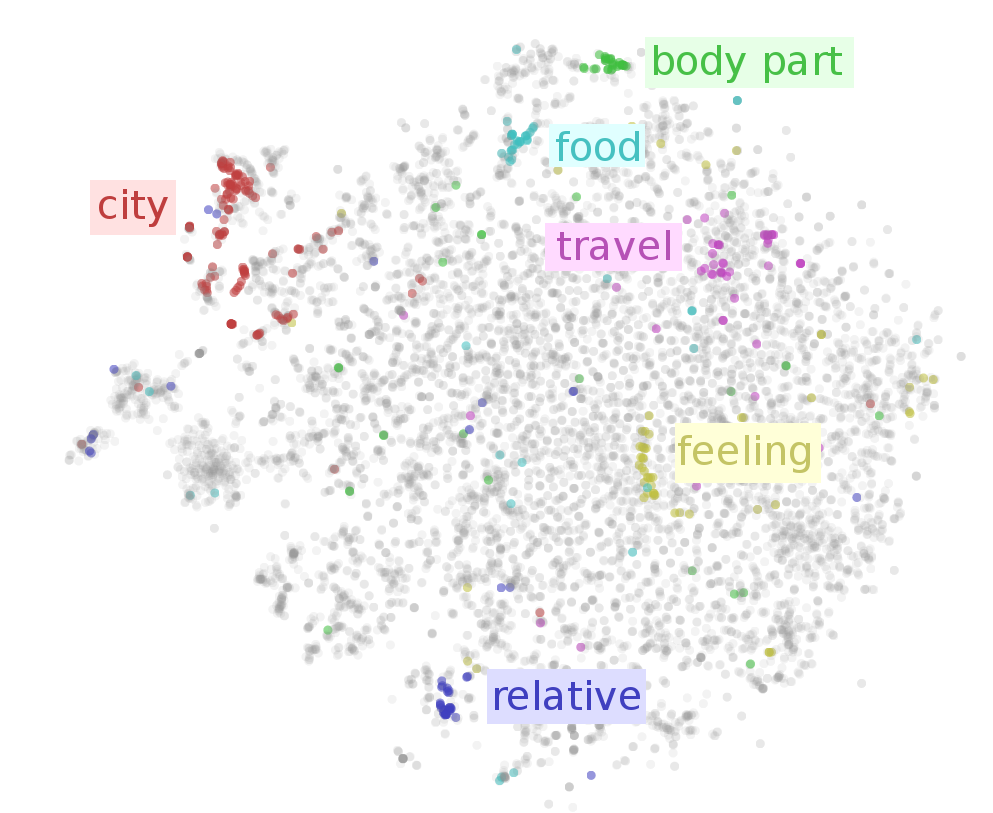
\includegraphics[width=0.3\textwidth]{Images/5.Theoretical_Background/word_embeddings_example.png}
    \caption{Example of Word Embedding representation in 2D space, From \cite{word-embedding-example}}
    \label{fig:word_embedding}
\end{figure}

There are some common word embedding models, such as Word2Vec, GloVe, FastText, etc. 

\subsection{Word2Vec}
Word2Vec is the popular word embedding technique. It was introduced by a team of researchers of Google, led by Tomas Mikolov in 2013 \cite{word2vec-paper-publication}. The key idea of Word2Vec is to learn word embedding by training a simple neural network. There are two main architectures for Word2Vec: Continuous Bag of Words (CBOW) and Skip-gram.
\begin{itemize}
    \item \textbf{Continuous Bag of Words (CBOW)}: The CBOW model predicts the current word based on the context. The CBOW architecture is similar to the feed-forward neural network, but it does not have the non-linear hidden layer to remove the computational complexity and the projection layer is shared for all words. The projection layer refers specifically to the layer responsible for transforming the input data (e.g., one-hot encoded vectors representing words) into a continuous vector space. The model architecture is shown in Figure \ref{fig:cbow_vs_skipgram}. 
    \item \textbf{Skip-gram}: The second architecture is similar to CBOW, but instead of predicting the current word based on the context, it tries to predict the surrounding words give the current word.
\end{itemize}

\begin{figure}[ht]
    \centering
    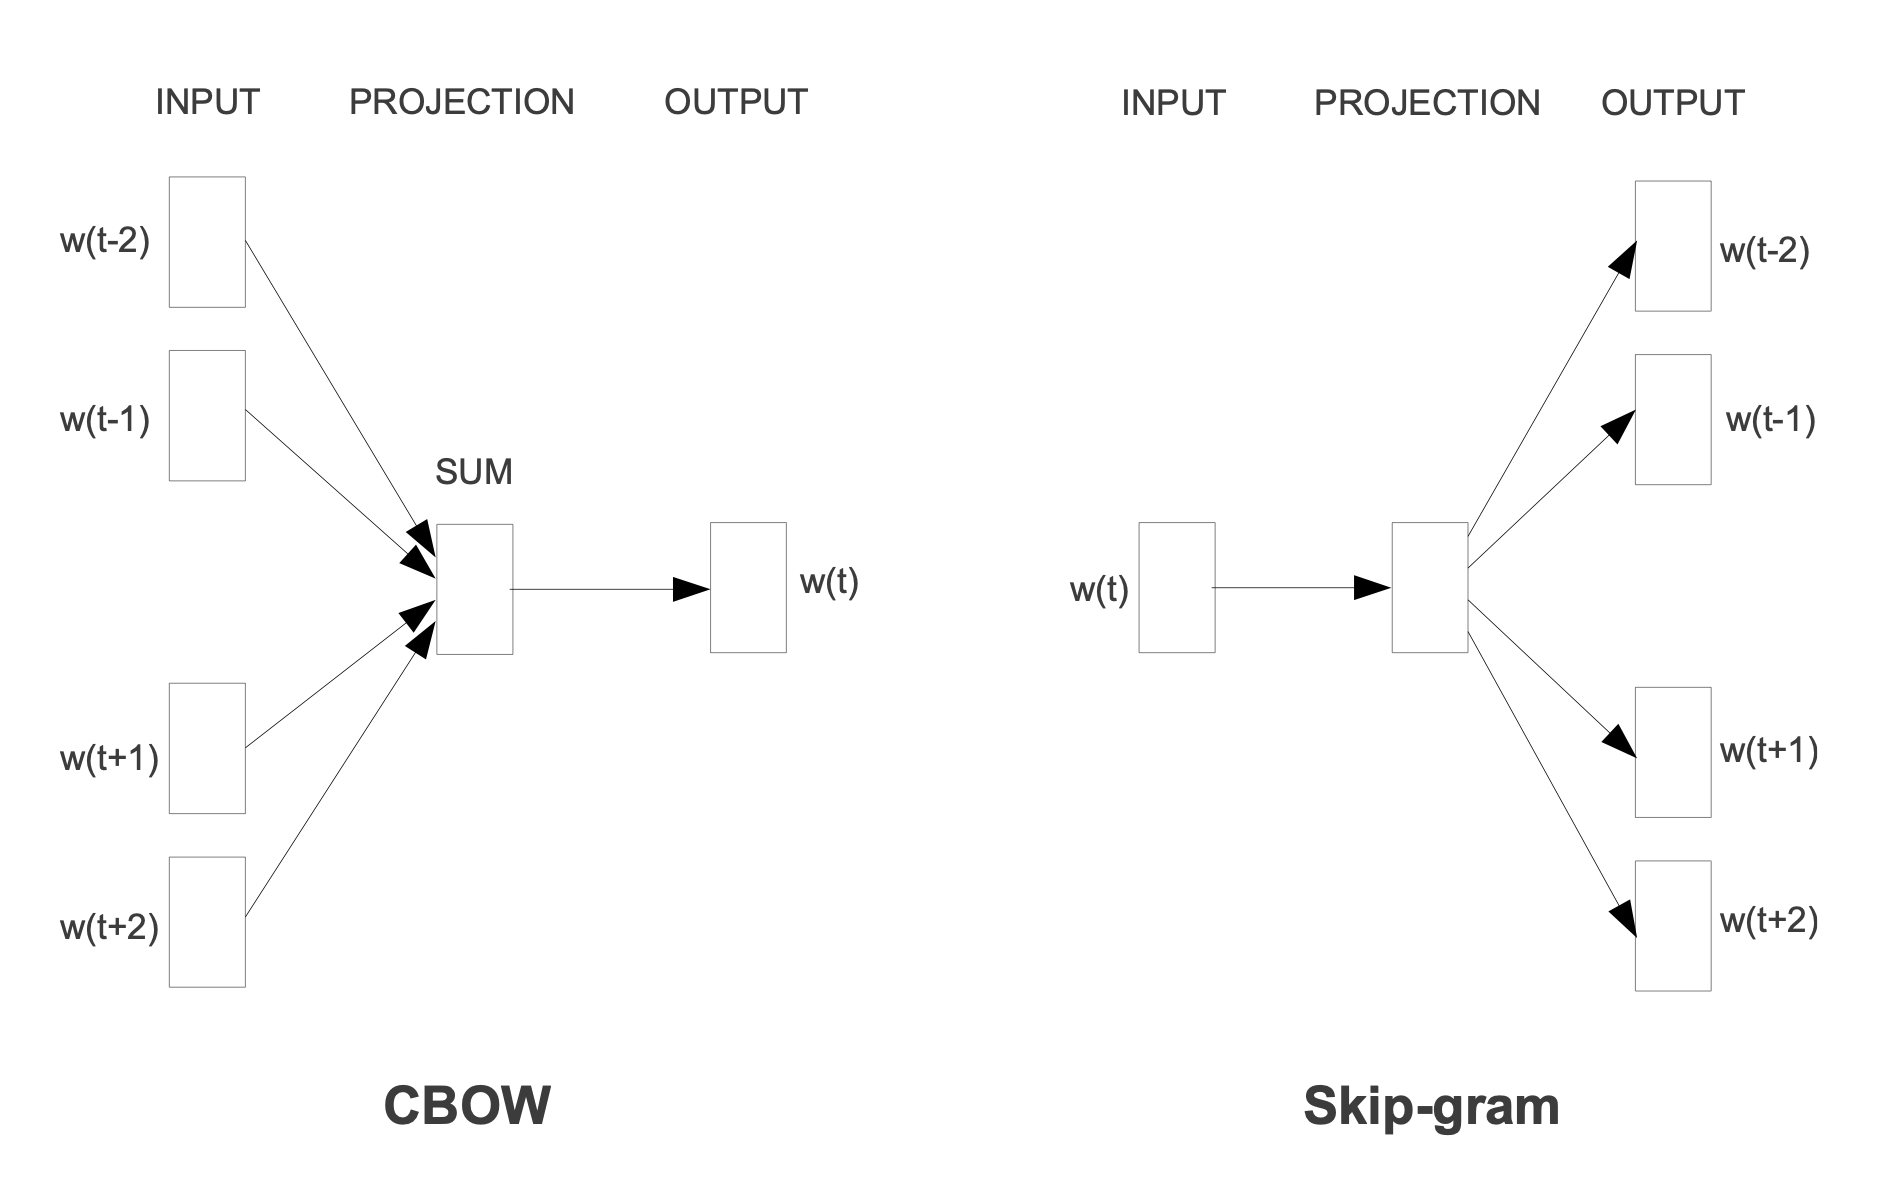
\includegraphics[width=0.8\textwidth]{Images/5.Theoretical_Background/cbow_vs_skipgram.png}
    \caption{The CBOW architecture predicts the current word based on the context, and the Skip-gram predicts surrounding words given the current word, From \cite{word2vec-paper-publication}}
    \label{fig:cbow_vs_skipgram}
\end{figure}

The training process involves backward propagation which adjusts the weights of the projection layer. The output of the projection layer is the word embedding that we want to get.

\subsection{Language Model for Word Embedding}
Although the pre-trained word embedding methods, such as Word2Vec, GloVe, FastText, etc can represent the word in the vector format, these are non-contextual word embedding. Because they can not capture the context of the words. For example, the word "Apple" has different meanings in the sentences "Apple releases the new MacbookPro" and "Apples are a good source of vitamin C". The word "Apple" in the first sentence refers to the technology company while the word "Apple" in the second sentence refers to the fruit. The traditional word embedding methods only represent the word "Apple" with one fixed vector, so it cannot distinguish these two meanings of the word "Apple".

The Language Model for Word Embedding technique uses the language model to create contextual word embeddings. Some popular Language Models for Word Embedding are ELMo, BERT, GPT, etc. These language models can capture the context of the words, due to the model architecture using some Sequence Neural Networks like ELMo or using transformer architecture like BERT. The architecture of these language models will be discussed in the next sections.

\section{Recurrent Neural Network (RNN)}
A Recurrent Neural Network (RNN) is a type of neural network model to deal with sequential data. Sequential data is data arranged in sequences such as text, speech, and time series, where the order of the data point is important. The RNN models allow the information to persist through the time steps, so it can capture the context of the words. For that reason, RNN models are widely used in the Natural Language Processing field.

\subsection{Architecture of FeedForward Neural Network}
Before going into the architecture of RNN models, we need to understand why the feedforward neural network models are limited in their ability to handle sequential data. Consider the feedforward neural network in Figure \ref{fig:feedforward_architecture}, the output $y_{i}$ only depends on the input layer, but there are some problems that the output $y_{i}$ also depend on the previous output $y_{j}$, $y_{j-1}$, $y_{j-2}$, etc. For example, in the Part-of-Speech tagging, if the model already has the two previous words as nouns and verbs respectively, then the current word is likely to be a noun. There are some relationships between the words in the sentence, but with the architecture, the feedforward neural network cannot capture these relationships.

\begin{figure}[ht]
    \centering
    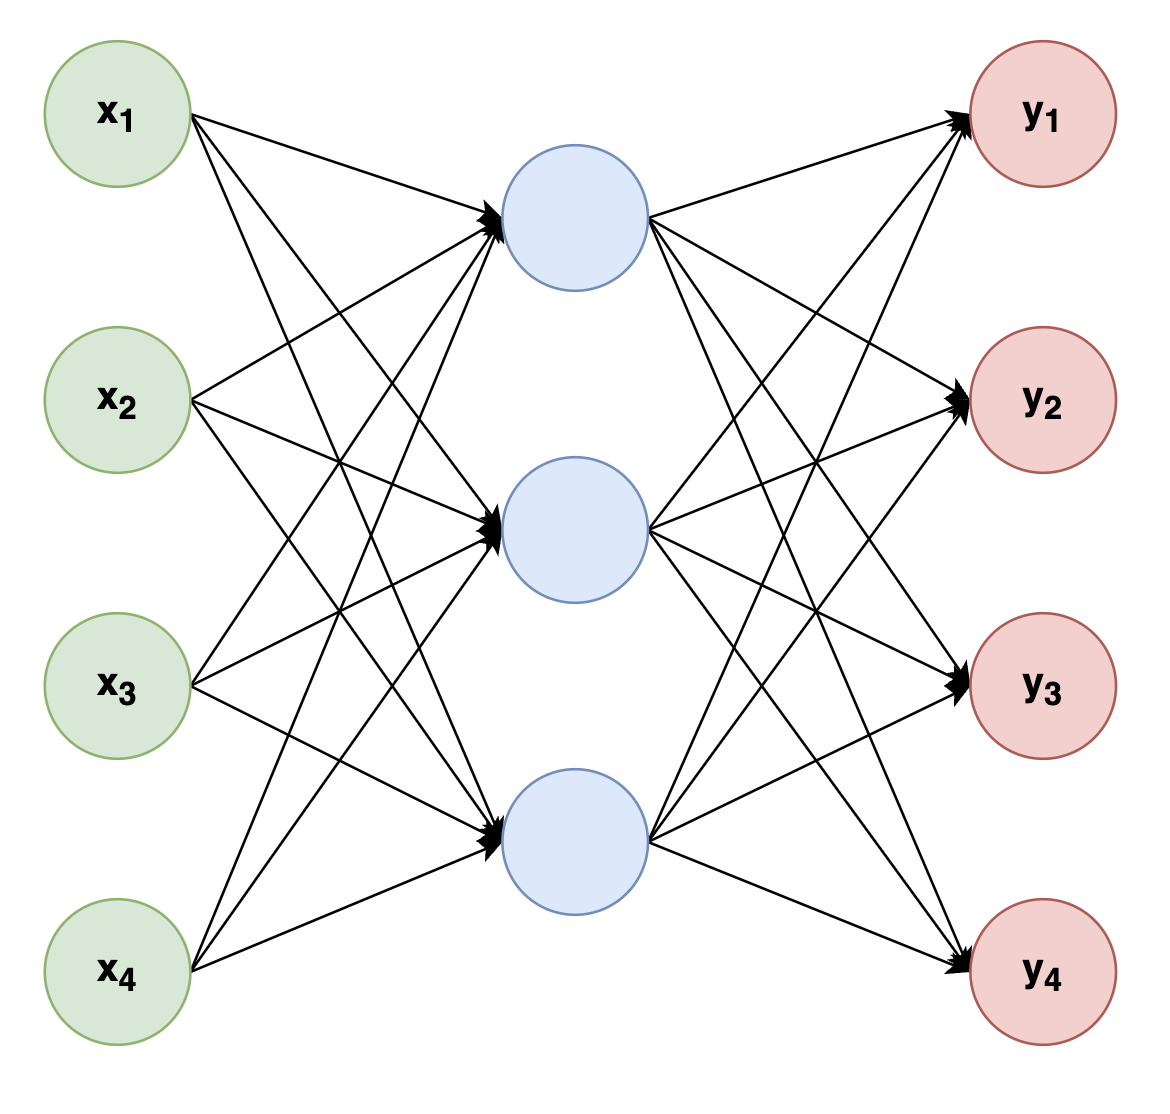
\includegraphics[width=0.4\textwidth]{Images/5.Theoretical_Background/feedforward_architecture.png}
    \caption{The architecture of feedforward neural network}
    \label{fig:feedforward_architecture}
\end{figure}

One major drawback of the feedforward neural network is that it only accepts the fixed-length input. However, the length of the sequential data is not fixed, so we need a model that can accept the variable-length input.

\subsection{Architecture of Recurrent Neural Network}
To solve the problem of feedforward neural networks, the Recurrent Neural Network (RNN) has a feedback loop that allows previous outputs to be used as inputs. The architecture of RNN is shown in Figure \ref{fig:rnn_fold} where the feedback loop is the red line. Another way to visualize the RNN architecture is to unfold the RNN into the sequence of the feedforward neural network as shown in Figure \ref{fig:rnn_unfold}

\begin{figure}[ht]
    \centering
    \begin{subfigure}[b]{0.3\textwidth}
        \centering
        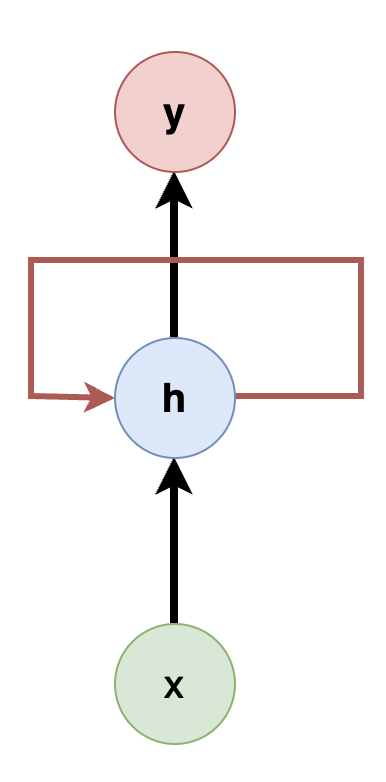
\includegraphics[height=0.25\textheight]{Images/5.Theoretical_Background/rnn_fold.png}
        \caption{RNN folded}
        \label{fig:rnn_fold}
    \end{subfigure}
    \begin{subfigure}[b]{0.65\textwidth}
        \centering
        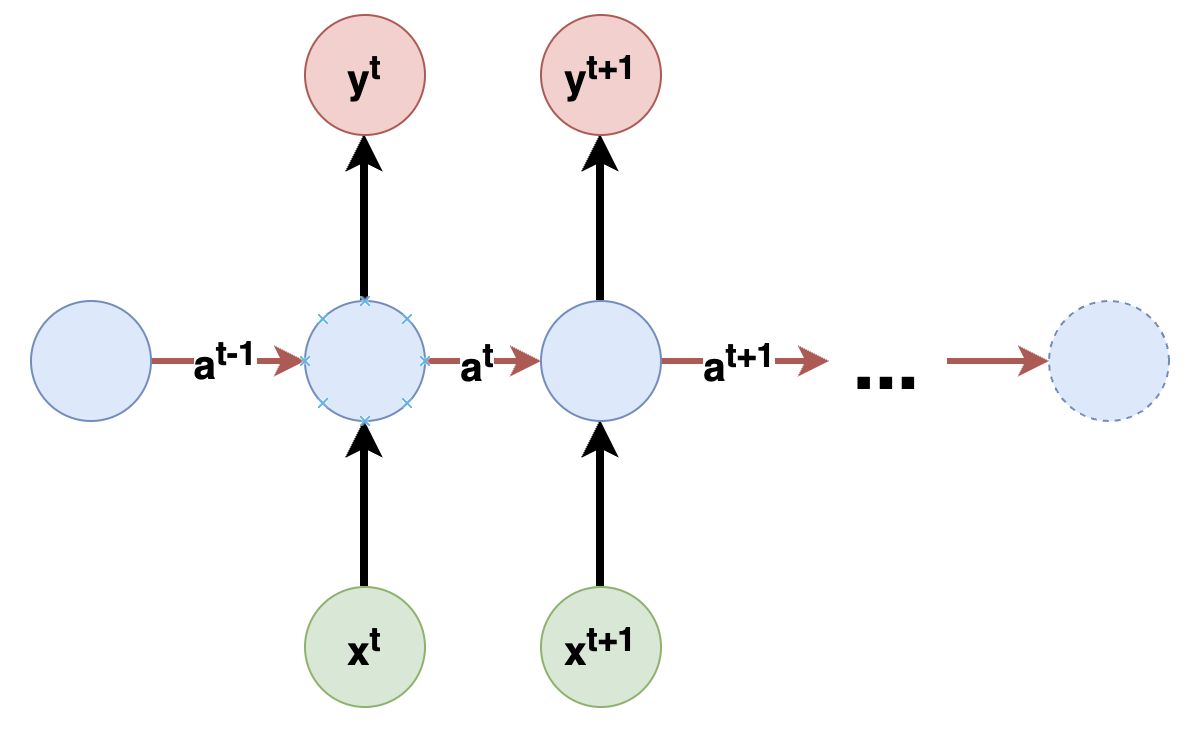
\includegraphics[height=0.25\textheight]{Images/5.Theoretical_Background/rnn_unfold.png}
        \caption{RNN unfolded}
        \label{fig:rnn_unfold}
    \end{subfigure}
    \caption{The architecture of RNN}
\end{figure}

The basic idea behind RNN is to use the hidden state $a^{<t-1>}$ from the previous time step as the input for the current step. The output $y^{<t>}$ and the hidden state $a^{<t>}$ is calculated as follows:

\begin{align*}
    a^{<t>} &= g_{1}(W_{aa}a^{<t-1>} + W_{ax}x^{<t>} + b_a) \\
    y^{<t>} &= g_{2}(W_{ya}a^{<t>} + b_y)
\end{align*}

\noindent where $g_{1}$ and $g_{2}$ are the activation functions, $W_{aa}$, $W_{ax}$, $W_{ya}$, are the weight matrices, $b_a$ and $b_y$ are the bias vectors. All of these parameters are the same over the time steps and are trained during the training process.

\subsection{The applications of RNN models}
There are many applications of RNN in the Natural Language Processing field such as text classification, name entity recognition, machine translation, etc. Based on the application, the RNN model can have different architectures. The RNN architectures and their applications are shown in Table \ref{tab:rnn_architecture}.

\begin{longtable}[ht]{| l | c | l |}
    \hline
    Type of RNN & Architecture & Application \\
    \hline
    One-to-Many & 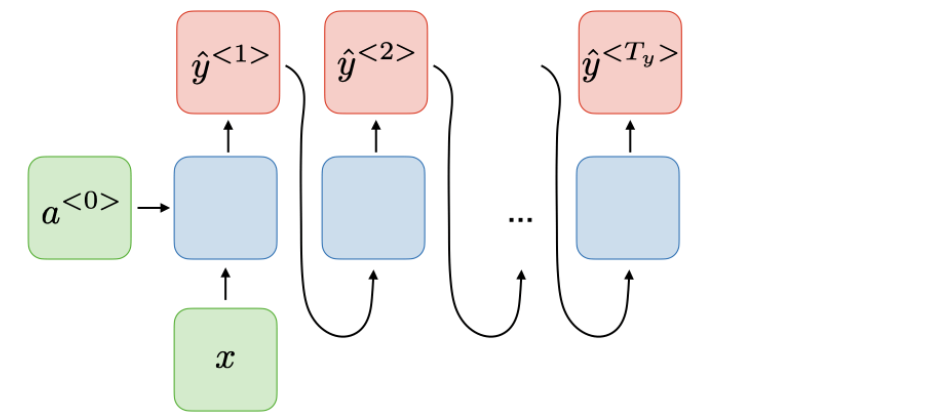
\includegraphics[width=0.5\textwidth]{Images/5.Theoretical_Background/rnn_one_to_many.png} & Text generation \\
    \hline
    Many-to-One & 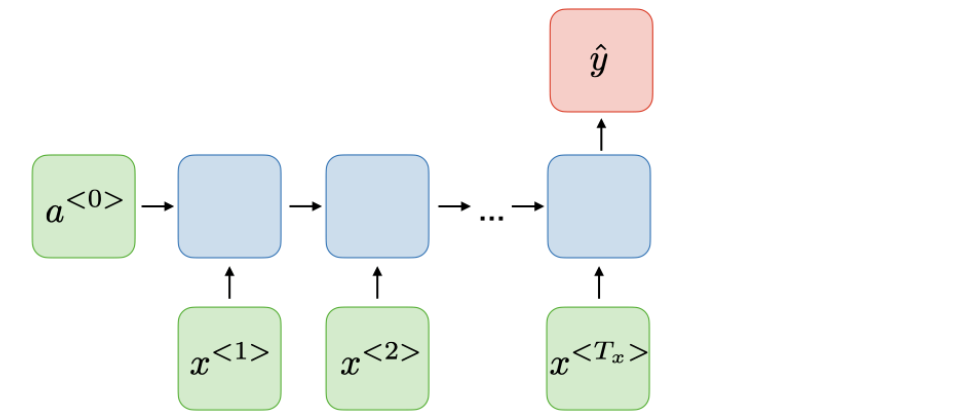
\includegraphics[width=0.5\textwidth]{Images/5.Theoretical_Background/rnn_many_to_one.png} & Text classification \\
    \hline
    Many-to-Many & 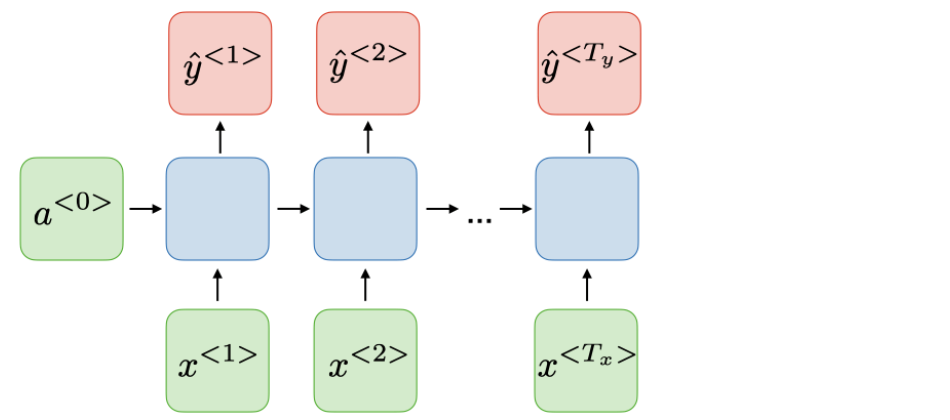
\includegraphics[width=0.5\textwidth]{Images/5.Theoretical_Background/rnn_many_to_many.png} & Name entity recognition \\
    \hline
    \caption{Different architectures of RNN}
    \label{tab:rnn_architecture}
\end{longtable}

\subsection{Disadvantages of RNN}
The training process of traditional RNN models consists of forward propagation (calculate the output from the beginning to the last time step) and backward propagation (calculate the gradients between the loss function and the parameters in the backward direction). Then these gradients are used to update the parameters. In the backward propagation process, the gradients can be very small or large. When the gradients are minimal, the parameters will not be updated, so the model fails to learn. It is called the vanishing gradient problem. Another problem is that the gradients can become exponentially large, so the model becomes very unstable and fails to optimize the weight matrix. It is called the exploding gradient problem. These problems make the training process of RNN models very difficult and unstable.

Besides, the information in RNN is propagated step by step from the first cell to the current cell, through each time step, the information is gradually lost, so the output of the RNN models mainly depends on the recent time steps. This leads to the problem that the RNN models cannot capture the long-term dependencies between the words.

\section{Long Short-Term Memory (LSTM)}
LSTM is a type of Recurrent Neural Network (RNN). The LSTM can deal with the vanishing gradient problem encountered by traditional RNNs. 

\subsection{LSTM architecture}
Consider the RNN cell and the LSTM cell in Figure \ref{fig:rnn_cell_vs_lstm_cell}. Similar to the RNN cell, the LSTM cell has the hidden state $a^{t}$. In addition to that, the LSTM also has a cell state represented by $c^{t-1}$ and $c^{t}$. The hidden state $a^{t}$ is used to capture the dependencies between the short-range time steps, so it is considered as the short-term memory. In contrast, the cell state $c^{t}$ could capture the dependencies between the long-range time steps, so it is considered as the long-term memory.

\begin{figure}[ht]
    \centering
    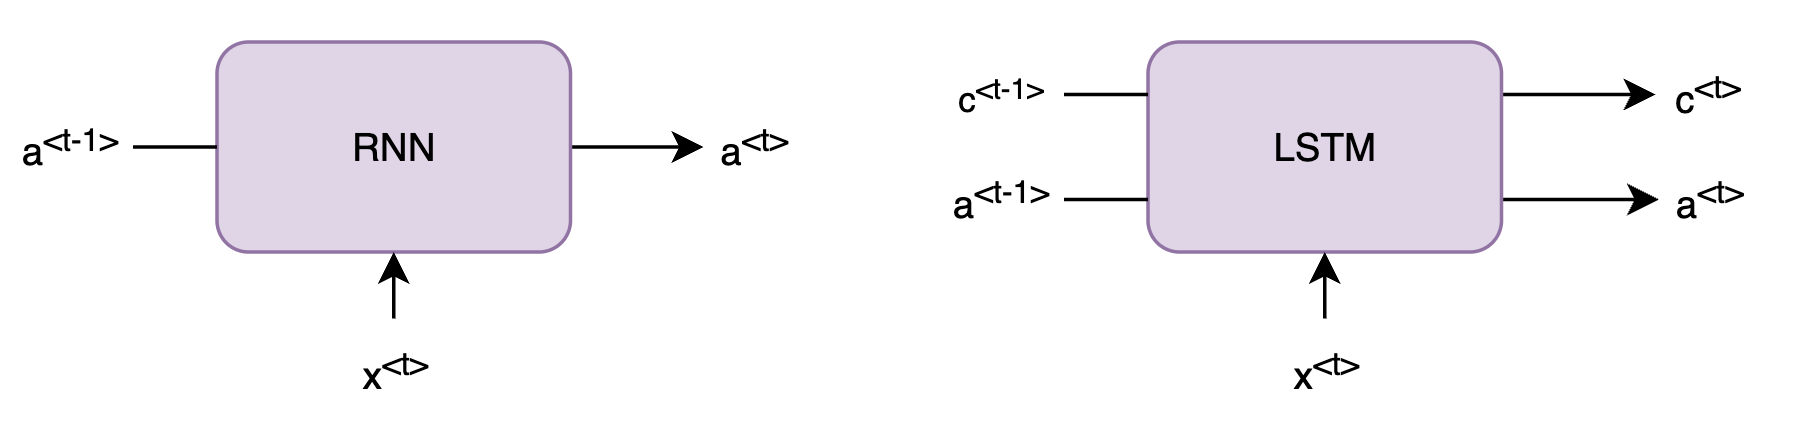
\includegraphics[width=0.7\textwidth]{Images/5.Theoretical_Background/rnn_vs_lstm_cell.png}
    \caption{The RNN cell and the LSTM cell}
    \label{fig:rnn_cell_vs_lstm_cell}
\end{figure}

The LSTM cell has 3 gates: the forget gate ($\Gamma_f$), the update gate($\Gamma_u$), and the output gate($\Gamma_o$). These gates control the flow of information through the cell. We have the following equations to calculate the gates and the cell state $c^{t}$:

\begin{align}
    \Gamma_f &= \sigma(W_f[a^{t-1}, x^{t}] + b_f) \\
    \Gamma_u &= \sigma(W_u[a^{t-1}, x^{t}] + b_u) \\
    \Gamma_o &= \sigma(W_o[a^{t-1}, x^{t}] + b_o) \\
    \tilde{c}^{t} &= tanh(W_c[a^{t-1}, x^{t}] + b_c) \label{eq:calcuate_c_tilde} \\
    c^{t} &= \Gamma_f * c^{t-1} + \Gamma_u * \tilde{c}^{t} \label{eq:calculate_c}\\
    a^{t} &= \Gamma_o * tanh(c^{t})
\end{align}

Based on the 3 first equations, we know that all the gates in the LSTM cell are calculated based on the previous hidden state $a^{t-1}$ and the current input $x^{t}$. The value of these three gates is between 0 and 1. In each cell, we have $\tilde{c}^{t}$ which is the candidate for the cell state $c^{t}$, representing the information in that cell. In equation \ref{eq:calculate_c}, the forget gate $\Gamma_f$ and the update gate $\Gamma_u$ decide which information to keep and which information to throw away. When the forget gate is nearly zero, it means the information $\tilde{c}^t$ in this cell is important and needs to be kept for the long term. In contrast, if the update gate is nearly zero, it means the information $\tilde{c}^t$ in this cell is not important and needs to be thrown away. So the $c^{t-1}$ is passed to the next cell. 

To sum up, the LSTM model can decide which information to keep and which information to throw away throughout the time steps. This allows the LSTM model to capture the important information for the long term and avoid the vanishing gradient problem.

\subsection{Bidirectional LSTM (BiLSTM)}
In some real scenarios, especially in the Natural Language Processing field, we need to get information from both the past and the future. It means that we need to consider the sequential data from both left to right and right to left directions. For example, two sentences: "Apple releases the new iPhone 12" and "Apple is a good source of vitamin C". With the traditional RNN models or the LSTM models, we only consider the context on the left of the words. So with these models, we can not distinguish the two meanings of the word "Apple". So we need a model that can capture the context of both sides of the word. That is the BiLSTM model.

The BiLSTM model consists of two LSTM layers, one layer processes the input sequence from the beginning to the end, and the other layer processes the input sequence from the end to the beginning. The output of the BiLSTM model is the concatenation of the outputs of the two LSTM layers. With this architecture, the BiLSTM model can capture the context of the previous words and the next words, so it is widely used in the Natural Language Processing field. The architecture of the BiLSTM model is shown in Figure \ref{fig:bilstm_architecture}.

\begin{figure}[ht]
    \centering
    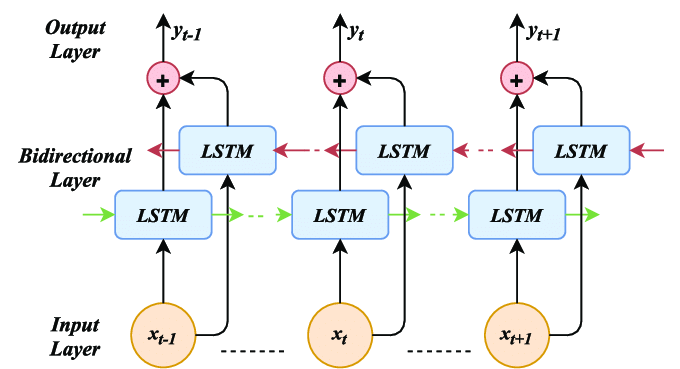
\includegraphics[width=0.8\textwidth]{Images/5.Theoretical_Background/bilstm_architecture.png}
    \caption{The architecture of the BiLSTM model, Source \cite{bilstm_medium} }
    \label{fig:bilstm_architecture}
\end{figure}

\section{Sequence to Sequence (Seq2Seq) Model}
The Sequence to Sequence model is a type of RNN model that takes a sequence of data (words, letters, time series data) as input and outputs another sequence of data. This model is applied to solve Natural Language Problems like machine translation, text summarization, question answering, etc...

There are two main components in the Seq2Seq model: the encoder and the decoder. Both the encoder and decoder are RNN models, usually LSTM models. The encoder takes the input sequence and encodes it into vectors (in the case of LSTM, these are the last hidden state and the cell state). The decoder takes these vectors from the encoder and decodes them into the output sequence. The architecture of the Seq2Seq model is shown in Figure \ref{fig:seq2seq_architecture}

\begin{figure}[ht]
    \centering
    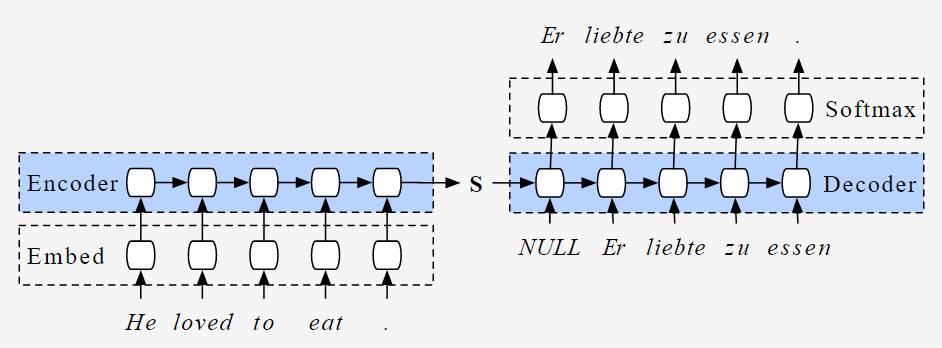
\includegraphics[width=0.8\textwidth]{Images/5.Theoretical_Background/seq2seq_architecture.png}
    \caption{Overall architecture of the Seq2Seq model, Source \cite{seq2seq_analyticsvidhya}}
    \label{fig:seq2seq_architecture}
\end{figure}

A problem with the original Seq2Seq model is that a neural network needs to compress all information of the input sequence into a fixed-length vector. This makes the model difficult to learn and deal with the long sentences. \cite{bahdanau2016neural}. The attention mechanism is the extension of the encoder-decoder architecture that solves this problem. Instead of encoding the whole input sentence, the attention mechanism allows the decoder to focus on the relevant parts of the input sentence when decoding each word. The attention mechanism is introduced in the next section.

\section{Attention}
In Psychology, attention is the human ability to selectively concentrate on one or a few things and ignore others. The Attention mechanism in NLP proposed in 2015 by Bahdanau et al in \cite{bahdanau2016neural} was inspired by this human ability. The key idea of the attention mechanism is at each time step, the decoder decides which part of the input sequence to focus on. To understand the attention mechanism, we consider the machine translation task.

We have the input sentence $x_1, x_2, x_3, ..., x_m$ in language A, and translation can be thought of as finding the output sentence $y_1, y_2, y_3, ..., y_n$ in language B. We use the encoder-decoder with an attention mechanism similar to Figure \ref{fig:attention_architecture} to solve this problem. The first step is that the encoder maps the input sentence $x_1, x_2, x_3, ..., x_m$ to a sequence of hidden states $s_1, s_2, s_3, ..., s_m$. Given the hidden states s, in each decoder time step, this model calculates the attention score between the decoder state $h_t$ and the encoder state $s_k$. The attention score shows how relevant is the source token k for target step t. Then it computes the attention weights by applying the softmax function to all the attention scores in the previous step. Next, we compute the attention output, using the formula $c^t = \sum_{k=1}^m a_k^t*s_k$. When we have the attention output $c^t$, we pass it along with the previous decoder state $h_{t-1}$ to predict the current output $h_t$. 

\begin{figure}[ht]
    \centering
    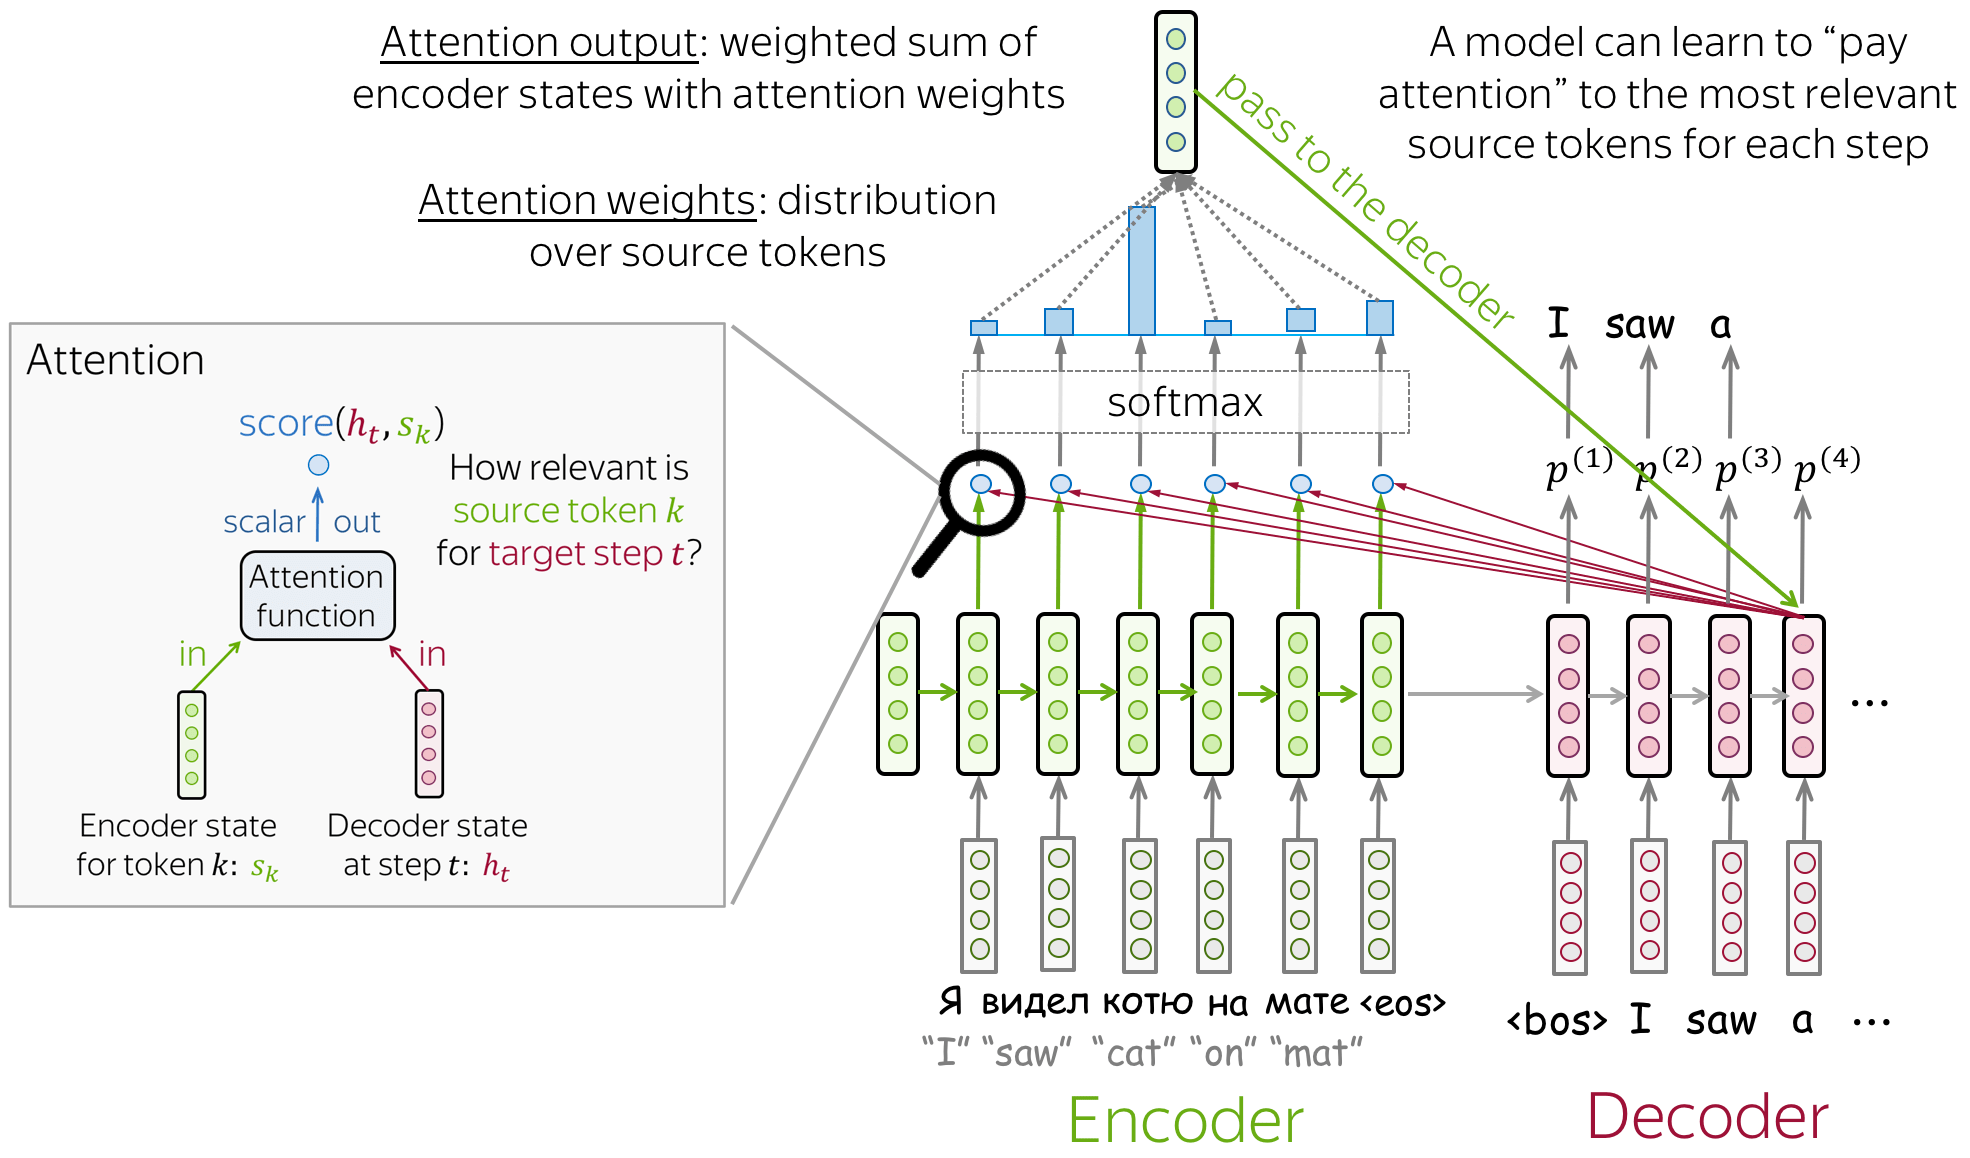
\includegraphics[width=0.8\textwidth]{Images/5.Theoretical_Background/attention_architecture.png}
    \caption{The architecture of the attention mechanism, Source \cite{voita2020nlpCourse}}
    \label{fig:attention_architecture}
\end{figure}

\section{Transformer}
The Transformer architecture is a neural network architecture introduced in the paper titled "Attention is All You Need" by Vaswani et al. in 2017 \cite{attentionIsAllYouNeed}. This is a breakthrough in the field of NLP because, at that time, the RNN models were considered state-of-the-art approaches to handle sequential data, especially in sequence modeling. However, the transformer does not use any of the RNN models, instead, it uses entirely the attention mechanism to capture the dependencies between input and output. The Transformer architecture allows the encoding and decoding at all time steps to be parallelized, so it is faster than the RNN models. The architecture of the Transformer is shown in Figure \ref{fig:transformer_architecture}. To understand the Transformer architecture, firstly, we need to understand the self-attention mechanism.

\begin{figure}[ht]
    \centering
    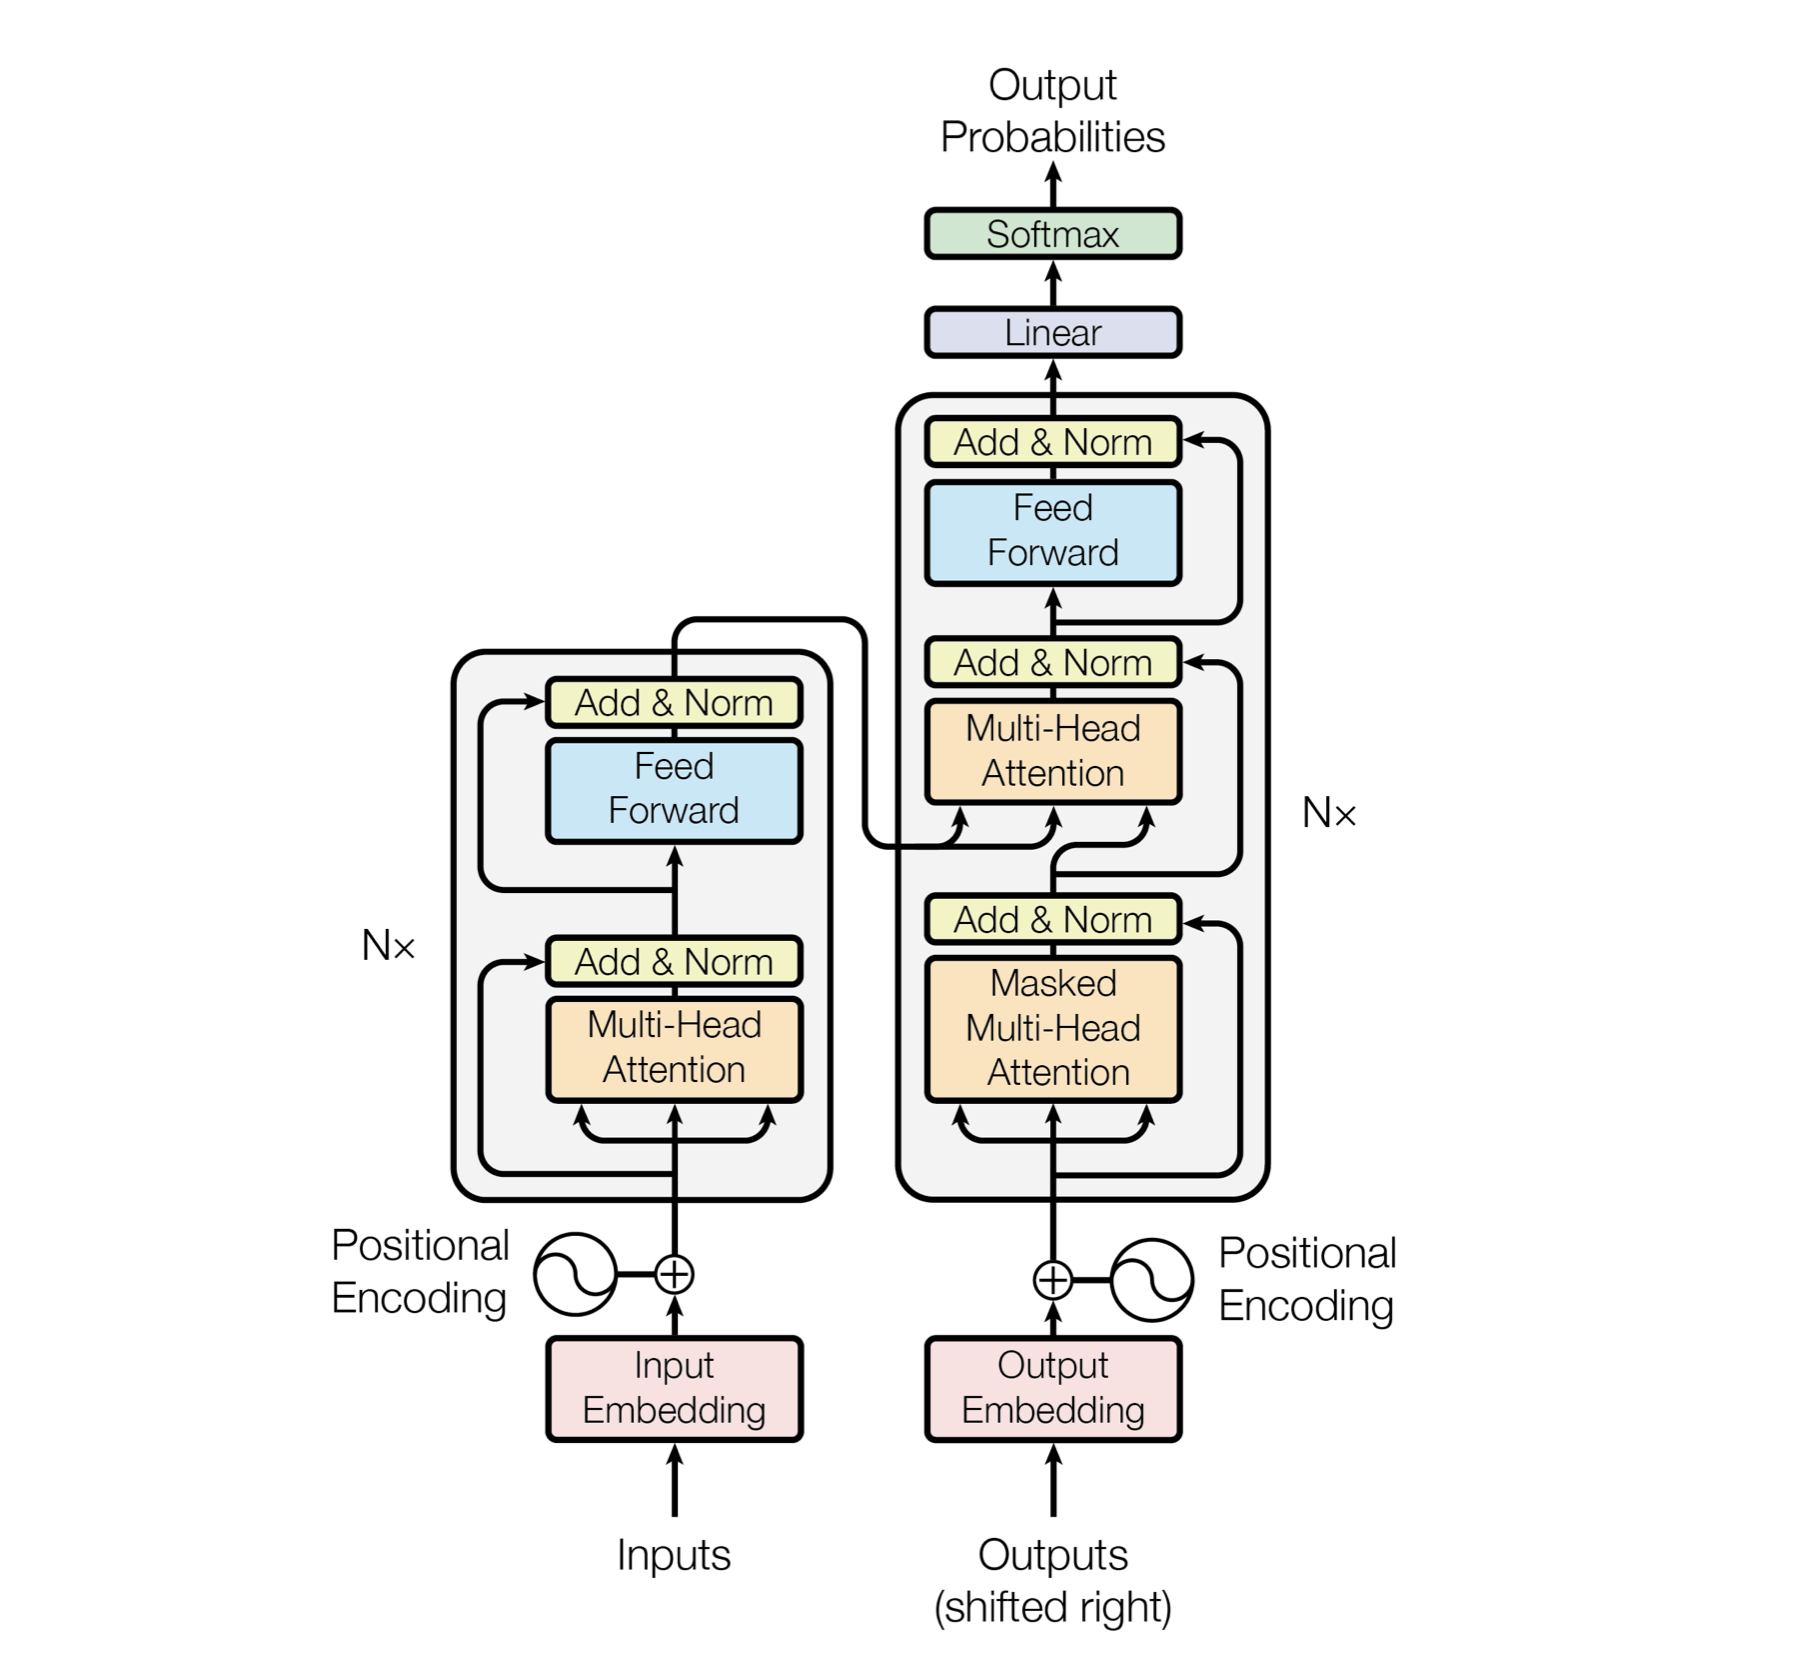
\includegraphics[width=0.8\textwidth]{Images/5.Theoretical_Background/transformer_architecture.png}
    \caption{The architecture of the Transformer proposed in \cite{attentionIsAllYouNeed}}
    \label{fig:transformer_architecture}
\end{figure}

\subsection{Self-Attention mechanism}
Self-Attention mechanism computes the attention score between every pair of words in the input sequence. The attention score shows how relevant is the word $x_j$ for the word $x_i$. The attention score is calculated as follows: 
\begin{enumerate}
    \item Each input token receives three representations: query, key and value.
    \item The attention score between the word $x_i$ and the word $x_j$ is calculated as the dot product between the query of the word $x_i$ and the key of the word $x_j$. The self-attention mechanism also calculates the attention score between the word and itself. 
    \item The weights are calculated by applying the softmax function to the attention scores.
    \item The attention output is calculated as the weighted sum of the value of all words in the input sequence. 
\end{enumerate}

\noindent After applying the self-attention mechanism, we get the output is the same as the input sequence, but the information of each word is updated based on the information of the other words in the input sequence. The self-attention mechanism is shown in Figure \ref{fig:self_attention_mechanism}.

\begin{figure}[ht]
    \centering
    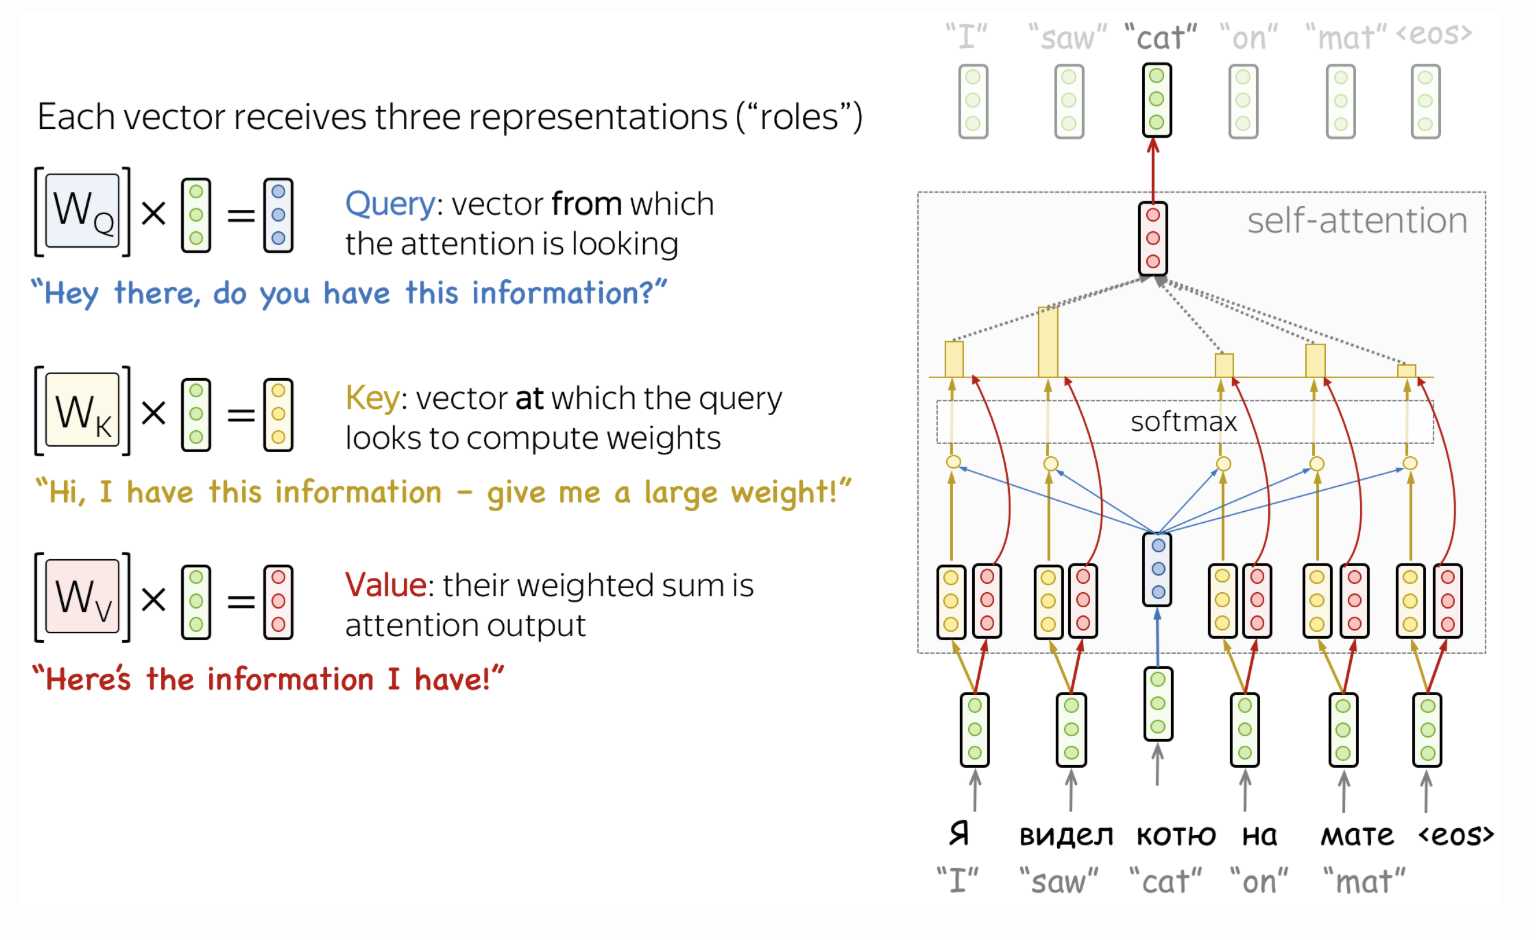
\includegraphics[width=0.8\textwidth]{Images/5.Theoretical_Background/self_attention_mechanism.png}
    \caption{The self-attention mechanism, Source \cite{voita2020nlpCourse}}
    \label{fig:self_attention_mechanism}
\end{figure}

The Self-Attention layers with different parameters can be stacked together to form the Multi-Head Attention layer. The Multi-Head Attention layer allows the model to capture different relationships between the words.

\subsection{Positional Encoding layer}
Because the Transformer does not use any of the RNN models, it cannot capture the position of the words in the input sequence. The Positional Encoding layer is used to solve this problem. The Positional Encoding layer adds the positional information to the input sequence. The Positional Encoding layer is calculated as follows:
\begin{align*}
    PE_{(pos, 2i)} &= sin(pos/10000^{2i/d_{model}}) \\
    PE_{(pos, 2i+1)} &= cos(pos/10000^{2i/d_{model}})
\end{align*}

\noindent Where pos is the position in the text and i is the vector dimension \cite{voita2020nlpCourse}

\subsection{FeedForward layer}
The FeedForward layer is a fully connected layer with a ReLU activation function. The FeedForward layer is used to transform the output of the Multi-Head Attention layer into the output of the Transformer and also process the new information from the Multi-Head Attention layer.

\section{BERT}
BERT (Bidirectional Encoder Representations from Transformers) is a language model proposed by Jacob Devlin et al. in 2018 \cite{bert_jacob}. BERT is a pre-trained language model that is pre-trained on a large corpus of text and can be fine-tuned for many NLP tasks. Besides, BERT is a bidirectional model, so it can capture the context of both sides of the words.



\chapter{System Analysis}
\section{Requirement elicitation}
\subsection{Stakeholders}
\begin{itemize}
    \item End users: tenants, landlords
    \item System owner: Ho Chi Minh City University of Technology
\end{itemize}
\subsection{Functional Requirements}
\begin{enumerate}
    \item Tenant
    \begin{itemize}
        \item The tenant can ask the chatbot to search for available rental listings based on places or neighborhoods. 
        \item The tenant can compare between 2 properties' information
        \item The tenant can filter available rental listings based on location, amenities, area, price, room type or specific keywords.
        \item The tenant can see the details of rental posts: accurate property listings with high-quality photos, comprehensive descriptions of the property and information about landlords.
        \item The tenant can save listings to a favorites shortlist so that the tenant can compare and revisit these properties later.
        \item The tenant can chat or contact the owner directly on the site.
        \item The tenant can verify property owner identities, conduct background checks, and review rental histories.
        \item The tenant can receive notifications about responses from the property owner, rental visits or any updates related to the rental application.
    \end{itemize}
    
    \item Landlord (property owner)
    \begin{itemize}
        \item The landlord can create and manage his/her rental property listing.
        \item The landlord can provide details information about the property.
        \item The landlord can ask the chat-bot system to create or manage rental property for them
        \item The landlord can verify tenant identities, conduct background checks, and review rental histories.
        \item The landlord can see the list of people who are interested in the property in their rental listings.
        \item The landlord can receive notifications about contact from tenant
        \item The landlord can chat or contact with tenant directly on the site
    \end{itemize}
    \item Others
    \begin{itemize}
        \item The system can get more rental data from the internet (other real-estate websites) and display on the system website.
        \item The system can provide related rental property based on the rental that the tenant is interested in.
        \item The system must be able to understand questions, and answer the questions from user in Vietnamese.
        \item The system must send notifications to the tenant about updated information in their favorite rental list.
    \end{itemize}
\end{enumerate}


\subsection{Non-functional Requirements}
\begin{enumerate}
    \item Usability
    \begin{itemize}
        \item The system has a user-friendly interface that the users can know how to use in less than 2 minutes.
        \item Tenant use and Landlord use should be clearly separated on the website.
    \end{itemize}
    \item Performance
    \begin{itemize}
        \item The system is able to process multiple (1000) users at a time.
        \item The system response time is less than 3 seconds.
        \item Search result accuracy should be at least 90\%.
        \item Unable to search response is less than 5\%.
        \item Beside the filter, the system can allow the user to search with natural language in the search engine
    \end{itemize}
    \item Security
    \begin{itemize}
        \item User conversations and account information must be protected.
    \end{itemize}
    \item Portability and compatibility
    \begin{itemize}
        \item The system should be compatible with three screen sizes (mobile, tablet, and desktop).
    \end{itemize}
    \item Development
    \begin{itemize}
        \item The system can be extendable to add more functions.
        \item The system can be extendable to process English.
    \end{itemize}
\end{enumerate}


\newpage
\section{Use case specification}
% short intro
Before using the application, user must sign up or log in with an account. Therefore, the requirement for Authentication and Authorization is already considered in the system, we will implement the Authentication module but not demonstrate it in the use-case diagrams for convenience. That way, we can pay more attention to the other modules. However, we must explain the authenticated flow in detail in activity diagrams because of some constraints that end-users of this website have to follow when use the apps. The main application, we call it Rental System, composes the features corresponding to 2 types of end-users: Tenant and Landlord. 

% %%%%%%%%% Rental system: Tenant view %%%%%%%%%%
\subsection{Rental system: Tenant view}
\subsubsection{Use case diagram}
\begin{figure}[H]
    \centering
    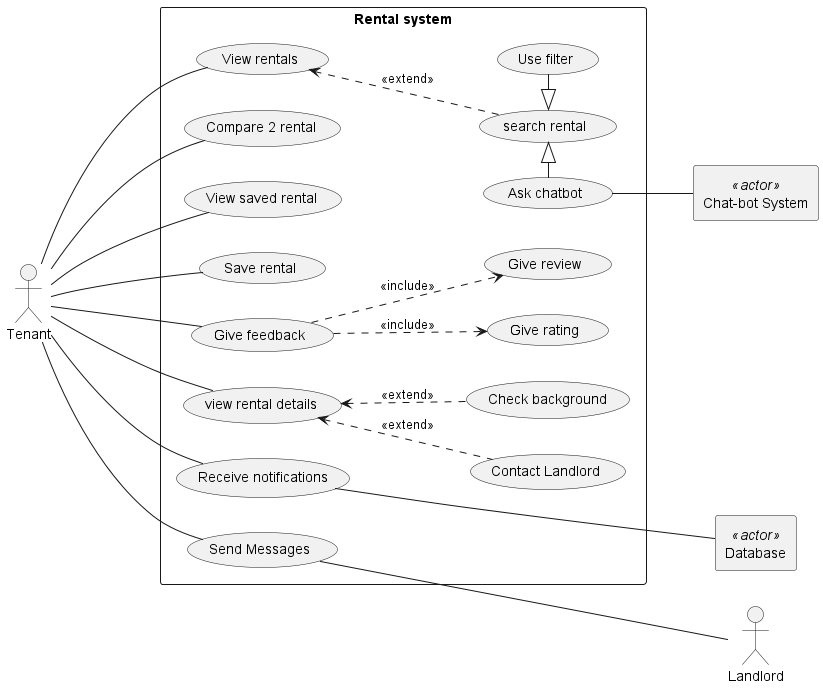
\includegraphics[width = 0.9\textwidth]{Images/rental_system_tenant.png}
    \caption{Use Case diagram: Rental System in Tenant view}
    \label{fig:enter-label}
\end{figure}

% %%%%%%%%%%%%%%%%%%%% Use case scenarios %%%%%%%%%%
\newpage
\subsubsection{Use-case Scenarios}

%%%----UC-01-------
\begin{table}[H]
    \centering
% \usepackage{tabularray}
\begin{longtblr}[
  label = none,
  entry = none,
]{
  width = \linewidth,
  colspec = {Q[140]Q[802]},
  hlines,
  vlines,
}
\textbf{Use-case ID}       & UC-01               \\
\textbf{Use-case Name}     & View rentals        \\
\textbf{Actor(s)}          & Tenant (Primary), Chat-bot System (Secondary)    \\
\textbf{Description}       & Tenant can see all the rentals general information in the main page or search page of application                    \\
\textbf{Pre-condition(s)}  & Tenant accesses to the website                                     \\
\textbf{Post-condition(s)} & The rentals listing will be shown on the main page of website        \\
\textbf{Trigger(s)}        & User is on the main page or search page                              \\
\textbf{Normal flow}       & {1. System display the list of available rentals on the page\\2. User scroll the page for more rentals\\3. System display rentals}                                 \\
\textbf{Alternative flow}  & {Alternative 1: at step 2\\ 2.1a. User choose the chat-bot to narrow down the list\\ 2.1b. System open the chat-bot\\ 2.1c. User search for rental using the chat-bot module (this will be explained with more details in use cases for chat-bot system)\\ 2.1d. Chat-bot return search result\\ Continue at step 3 of normal flow\\Alternative 2: at step 2\\  2.2a. User choose the filter to narrow down the list\\  2.2b. System open the filtering form\\  2.2c. User search for rental by completing and submitting the form\\  2.2d. System search for result\\ Continue at step 3 of normal flow} \\
\textbf{Exception flow}    & {Exception 1: No result found at step 2.1d or 2.2d\\ - If no rental information matches the requirement, then the system display "No rental result found" message to the tenant}                           \end{longtblr}
    \caption{Use case scenario: View list available rentals}
    \label{tab:usecase-scenario-view-rentals}
\end{table}



%%%----UC-02-------
\newpage
% \usepackage{tabularray}
\begin{table}[H]
    \centering
\begin{longtblr}[
  label = none,
  entry = none,
]{
  width = \linewidth,
  colspec = {Q[130]Q[797]},
  hlines,
  vlines,
}
\textbf{Use-case ID}       & UC-02               \\
\textbf{Use-case Name}     & View rental detail  \\
\textbf{Actor(s)}          & Tenant (Primary)    \\
\textbf{Description}       & Tenant can see all the rentals detail information                   \\
\textbf{Pre-condition(s)}  & User see the list of rentals in main page or search page           \\
\textbf{Post-condition(s)} & Tenant can see all the rentals detail information (accurate property listings with high-quality photos, comprehensive descriptions of the property and information about landlord)                      \\
\textbf{Trigger(s)}        & Tenant clicks on a rental post in the list of rental                \\
\textbf{Normal flow}       & {1. System routes to rental detail page
\\2. System display detail information about the rental
\\3. User return to the main page
\\4. System routes to the main page
\\End use case}                                  \\
\textbf{Alternative flow}  & {Alternative 1: at step 2 - Tenant want to check Landlord background
\\ 2.1a. Tenant click on Landlord Title in Landlord section
\\ 2.1b. System routes to Landlord detail page (more information: title, time register, reviews, ratings, related rental properties, contact information)
\\ 2.1c. User return to the rental detail page
\\ 2.2d. System routes to rental detail page
\\ Continue at step 3 of normal flow
\\Alternative 2: at step 2 or 2.1b - Tenant want to contact the Landlord
\\ 2.2a. Tenant clicks on Landlord contact button
\\ 2.2b. System open the message section
\\ 2.2c. User start sending message or calling
\\ 2.2d. User closes the message section
\\ 2.2e. User return to the rental detail page
\\ 2.2f. System routes to rental detail page
\\ Continue at step 3 of normal flow } \\
\textbf{Exception flow}    & No exception        \end{longtblr}
    \caption{Use case scenario: View rental detail information}
    \label{tab:usecase-scenario-view-rental-detail}
\end{table}              


%%%----UC-03-------
\newpage
\begin{table}[H]
    \centering
\begin{longtblr}[
  label = none,
  entry = none,
]{
  width = \linewidth,
  colspec = {Q[215]Q[727]},
  hlines,
  vlines,
}
\textbf{Use-case ID}       & UC-03                            \\
\textbf{Use-case Name}     & Compare 2 rentals                \\
\textbf{Actor(s)}          & Tenant (Primary)                 \\
\textbf{Description}       & Tenant can compare 2 rentals side by side                                                  \\
\textbf{Pre-condition(s)}  & Tenant see the list of rentals in main page or search page                                      \\
\textbf{Post-condition(s)} & The system show the information of 2 rental post side by side                                 \\
\textbf{Trigger(s)}        & Tenant clicks on "compare" button a rental post in the list of rental~                   \\
\textbf{Normal flow}       & {1. Tenant clicks on "compare" button of a rental post\\2. Tenant clicks on other rental post in the list~\\3. System routes to Compare page\\4. System shows the information side by side\\5. Tenant might return to the main page\\End use case} \\
\textbf{Alternative flow}  & No alternative
\\
\textbf{Exception flow}    & No exception        \end{longtblr}
    \caption{Use case scenario: Compare 2 rental information}
    \label{tab:usecase-scenario-compare-2-rentals}
\end{table}


%%-----UC-04----------
\newpage
\begin{table}[H]
    \centering
\begin{longtblr}[
  label = none,
  entry = none,
]{
  width = \linewidth,
  colspec = {Q[213]Q[731]},
  hlines,
  vlines,
}
\textbf{Use-case ID}       & UC-04                      \\
\textbf{Use-case Name}     & Save rental post           \\
\textbf{Actor(s)}          & Tenant (Primary)           \\
\textbf{Description}       & Tenant can save rental post into saved list for later reviewing                \\
\textbf{Pre-condition(s)}  & User see the list of rentals in main page or on the rental detail page       \\
\textbf{Post-condition(s)} & The rentals post added to the saved list                                          \\
\textbf{Trigger(s)}        & Tenant clicks the "Heart icon" on the rental post~                               \\
\textbf{Normal flow}       & {1. Tenant on the main page (show list of rental)\\2. Tenant clicks on "Heart icon" on the rental post\\3. System added the rental post to saved list\\4. System prompt message "Rental saved"\\End use case} \\
\textbf{Alternative flow}  & {Alternative 1: at step 1 - Tenant clicks to see rental detail\\~1.1a. System routes to rental detail page\\~1.1b. Tenant clicks on SSave rental" button\\~Continue in step 3 of normal flow}                 \\
\textbf{Exception flow}    & No exception               \end{longtblr}
    \caption{Use case scenario: Save rentals to saved list}
    \label{tab:usecase-scenario-save-rentals}
\end{table}

%--------UC-05---------
\newpage
\begin{table}[H]
    \centering
% \usepackage{tabularray}
\begin{longtblr}[
  label = none,
  entry = none,
]{
  width = \linewidth,
  colspec = {Q[138]Q[804]},
  hlines,
  vlines,
}
\textbf{Use-case ID}       & UC-05                      \\
\textbf{Use-case Name}     & View saved rentals         \\
\textbf{Actor(s)}          & Tenant (Primary)           \\
\textbf{Description}       & Tenant can see list of rentals post in saved list                              \\
\textbf{Pre-condition(s)}  & User logged in successfully                                            \\
\textbf{Post-condition(s)} & The saved rentals listing will be shown on the main page of website               \\
\textbf{Trigger(s)}        & Tenant click on the "Saved rentals" button                                         \\
\textbf{Normal flow}       & {1. Tenant click on the "Saved rentals" button\\2. System displays list of saved rental post on the saved section~\\End use case}  \\
\textbf{Alternative flow}  & No alternative             \\
\textbf{Exception flow}    & {Exception 1: at step 2 - the saved list is empty\\ - If the list is empty, tenant haven't save any rental post yet , then the system display "No rental result found" message to the tenant} 
\end{longtblr}
    \caption{Use case scenario: View saved rentals}
    \label{tab:usecase-scenario-view-saved-rentals}
\end{table}


%------UC-06-----
\newpage
\begin{table}[H]
    \centering
% \usepackage{tabularray}
\begin{longtblr}[
  label = none,
  entry = none,
]{
  width = \linewidth,
  colspec = {Q[165]Q[777]},
  hlines,
  vlines,
}
\textbf{Use-case ID}       & UC-06                        \\
\textbf{Use-case Name}     & Give feedback                \\
\textbf{Actor(s)}          & Tenant (Primary)             \\
\textbf{Description}       & Tenant can give feedback on the rental post about the rental expericence or about the Landlord                                                  \\
\textbf{Pre-condition(s)}  & No precondtion               \\
\textbf{Post-condition(s)} & System updates rating and review in rental information and Landlord profile         \\
\textbf{Trigger(s)}        & Tenant click on the "Star Icon" on the rental post or the "Feedback button" on the rental detail page                                        \\
\textbf{Normal flow}       & {1. Tenant clicks on "Star Icon" on the rental post\\2. System opens a Feedback form\\3. Tenant enters rating and reviews for the rental experience\\4. Tenant enters rating and reviews for the Landlord\\5. Tenant submits the form\\6. System updates rating and review information\\7. System closes the fom and prompts message "Feedback updated"\\End use case} \\
\textbf{Alternative flow}  & {Alternative 1: at step 1 - Tenant on the rental detail page\\~1.a. Tenant scrolls to review section\\~1.b. Tenant clicks on "Leave feedback" button\\~Continue at step 2 in normal flow}               \\
\textbf{Exception flow}    & No exception                 \end{longtblr}
    \caption{Use case scenario: Tenant leave feedback on rental experience and Landlord credibility}
    \label{tab:usecase-scenario-give-feedback}
\end{table}


%-----UC-07---------
\newpage
\begin{table}[H]
    \centering
% \usepackage{tabularray}
\begin{longtblr}[
  label = none,
  entry = none,
]{
  width = \linewidth,
  colspec = {Q[196]Q[746]},
  hlines,
  vlines,
}
\textbf{Use-case ID}       & UC-07                         \\
\textbf{Use-case Name}     & Receive notification          \\
\textbf{Actor(s)}          & Tenant (Primary), Database System (Secondary)              \\
\textbf{Description}       & Tenant receives notification when there are updates information in saved list           \\
\textbf{Pre-condition(s)}  & Tenant had saved rental post to favorite list~                                          \\
\textbf{Post-condition(s)} & System send notification into Tenant notification box and email                          \\
\textbf{Trigger(s)}        & Landlord updates rental listing information                                        \\
\textbf{Normal flows}      & {1. Landlord updates information in the rental listing\\2. System updates the information into databse\\3. System publishes updates to the tenant who saved the rental\\4. Tenant receives the notification\\End use case} \\
\textbf{Alternative flow}  & No alternative                \\
\textbf{Exception flow}    & {Exception 1: \\If Tenant have not saved any rental post, then when there is an updates, no notification will be sent.}                  \end{longtblr}
    \caption{Use case scenario: Tenant receive notification about updates information}
    \label{tab:usecase-scenario-receive-information}
\end{table}


%-----UC-08-------
\newpage
\begin{table}[H]
    \centering
% \usepackage{tabularray}
\begin{longtblr}[
  label = none,
  entry = none,
]{
  width = \linewidth,
  colspec = {Q[188]Q[754]},
  hlines,
  vlines,
}
\textbf{Use-case ID}       & UC-08                       \\
\textbf{Use-case Name}     & Send messages                 \\
\textbf{Actor(s)}          & Tenant (Primary), Landlord(secondary)                                        \\
\textbf{Description}       & Tenant want to send message to Landlord                                                \\
\textbf{Pre-condition(s)}  & Tenant had account and logged in successfully  \\
\textbf{Post-condition(s)} & Tenant can contact with Landlord~                                                  \\
\textbf{Trigger(s)}        & Tenant click on "Message Icon" on rental detail post, or on Landlord profile page~  \\
\textbf{Normal flows}      & {Normal flow 1: Tenant send message to Landlord for the first time\\1. Tenant clicks on the Icon\\2. System added Landlord into contact list\\3. System opens message section\\4. Tenant enters message into chat input\\5. System sends message to correspond Landlord\\6. Tenant click on "Close Button" the message section\\7. System closes the message section\\Use case ends} \\
\textbf{Alternative flow}  & {Alternative 1: at step 6 - Landlord responses\\1.1. Tenant receives message\\Return in step 5\\Alternative 2: Tenant contact with Landlord before\\2.1. Tenant clicks on "Message Icon" on the main page\\2.2. System opens the message section with chat list\\2.3. Tenant choose the existed Landlord\\Continue at step 3 in normal flow}                                     \\
\textbf{Exception flow}    & {No exception}
\end{longtblr}
    \caption{Use case scenario: Tenant sends message to Landlord}
    \label{tab:usecase-scenario-tenant-send-message}
\end{table}


%%%%%%%%%% Rental system: Landlord %%%%%%%%%%%%%%%
\newpage
\subsection{Rental system: Landlord view}
The same as Tenant
\subsubsection{Use case diagram}
\begin{figure}[H]
    \centering
    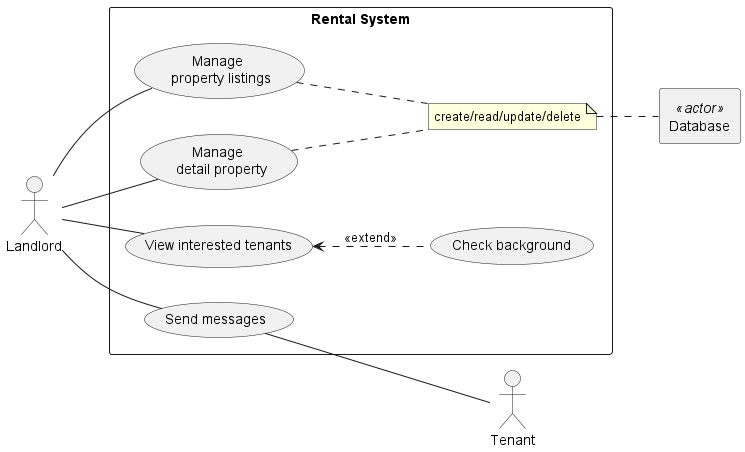
\includegraphics[width = \textwidth]{Images/rental_systen_landlord.png}
    \caption{Use Case diagram: Rental System in Landlord view}
    \label{fig:enter-label}
\end{figure}

\newpage
\subsubsection{Use case scenario}
%-------------UC-09-1---------------
\begin{table}[H]
    \centering
% \usepackage{tabularray}
\begin{longtblr}[
  label = none,
  entry = none,
]{
  width = \linewidth,
  colspec = {Q[160]Q[785]},
  hlines,
  vlines,
}
\textbf{Use-case ID}       & UC-09-1                    \\
\textbf{Use-case Name}     & Manage property listing - Create rental listing                                   \\
\textbf{Actor(s)}          & Landlord (primary), Database system (secondary)                             \\
\textbf{Description}       & Landlord have all the abilities to create a rental listing                    \\
\textbf{Pre-condition(s)}  & Landlord logged in successfully                                            \\
\textbf{Post-condition(s)} & System updates information into Database system, new rental post appears on Inventory list of Landlord                              \\
\textbf{Trigger(s)}        & Landlord click on "Create rental" option in main page                             \\
\textbf{Normal flows}      & {1. Landlord chooses Create option\\2. System opens the corresponding form\\3. Landlord enters the information\\4. Landlord submit the form\\5. System updates the information into Database\\6. System sends confirmation to Landlord\\End use case~~} \\
\textbf{Alternative flow}  & No alternative             \\
\textbf{Exception flow}    & Exception 1:~at step 4 - Landlord closes the form. Then system save the form as draft and end use case                                  \end{longtblr}
    \caption{Use case scenario: Landlord create new rental listing}
    \label{tab:usecase-scenario-create-rental}
\end{table}

%------------UC-09-2----------------------
\newpage
\begin{table}[H]
    \centering
% \usepackage{tabularray}
\begin{longtblr}[
  label = none,
  entry = none,
]{
  width = \linewidth,
  colspec = {Q[150]Q[837]},
  hlines,
  vlines,
}
\textbf{Use-case ID}       & UC-09-2                         \\
\textbf{Use-case Name}     & Manage property listing - Read/View rental inventory lists                             \\
\textbf{Actor(s)}          & Landlord (primary), Database system (secondary)                                           \\
\textbf{Description}       & Landlord can see all the rentals general information in the main page~                \\
\textbf{Pre-condition(s)}  & Landlord logged in successfully     \\
\textbf{Post-condition(s)} & The rental list will be shown on the main page of website                                  \\
\textbf{Trigger(s)}        & User is on the main page or search page                                                  \\
\textbf{Normal flow}       & {1. System display the list of all rentals inventory of Landlord with rental general information on the page\\2. If system can not display all rental inventories in the list, Landlord can scroll the page for more rentals\\3. System display more rentals\\End use case~}                                                       \\
\textbf{Alternative flow}  & {No Alternative} \\
\textbf{Exception flow}    & Exception 1: If Landlord have not create any rental inventory yet, the system will prompt the message "You haven't create any rental inventory yet" instead                                    \end{longtblr}
    \caption{Use case scenario: Landlord view rentals inventory list}
    \label{tab:usecase-scenario-view rentals}
\end{table}


%------------UC-09-3----------------------
\newpage
\begin{table}[H]
    \centering
% \usepackage{tabularray}
\begin{longtblr}[
  label = none,
  entry = none,
]{
  width = \linewidth,
  colspec = {Q[127]Q[815]},
  hlines,
  vlines,
}
\textbf{Use-case ID}       & UC-09-3                         \\
\textbf{Use-case Name}     & Manage property listing - Update rental listing                                        \\
\textbf{Actor(s)}          & Landlord (primary), Database system (secondary)                                           \\
\textbf{Description}       & Landlord can update the information in their rental listing                          \\
\textbf{Pre-condition(s)}  & Landlord logged in successfully, the rental post is created                     \\
\textbf{Post-condition(s)} & System updates information into Database system                                              \\
\textbf{Trigger(s)}        & Landlord click on "Edit" option in the rental post                                           \\
\textbf{Normal flows}      & {1. On the main Landlord page, there is a Inventory list (list of all rental post that Landlord has created), Landlord click on Edit button on the rental post~\\2. System opens the corresponding detail page of that rental post for updating information\\3. Landlord enters the information\\4. Landlord submit the updates\\5. System updates the information into Database\\6. System sends confirmation to Landlord\\End use case~~} \\
\textbf{Alternative flow}  & No alternative                  \\
\textbf{Exception flow}    & Exception 1:~at step 4 - Landlord closes the form. Then system abort the updating and keep the previous information and end use case               \end{longtblr}
    \caption{Use case scenario: Landlord updates information of rental inventory}
    \label{tab:usecase-scenario-update-rental}
\end{table}

%---------UC-09-4--------------
\newpage
\begin{table}[H]
    \centering
% \usepackage{tabularray}
\begin{longtblr}[
  label = none,
  entry = none,
]{
  width = \linewidth,
  colspec = {Q[150]Q[842]},
  hlines,
  vlines,
}
\textbf{Use-case ID}       & UC-09-4                           \\
\textbf{Use-case Name}     & Manage property listing - Delete rental inventory lists                                         \\
\textbf{Actor(s)}          & Landlord (primary), Database system (secondary)                                             \\
\textbf{Description}       & Landlord can delete a rental inventory in the main page~            \\
\textbf{Pre-condition(s)}  & Landlord has created some rental post in inventory list                                         \\
\textbf{Post-condition(s)} & The system updates to the Database, the rental post is deleted                           \\
\textbf{Trigger(s)}        & User clicks on "Delete" button on the rental post                                                \\
\textbf{Normal flow}       & {1. System display the list of all rentals inventory of Landlord with rental general information on the page\\2. Landlord clicks on "Delete" button on the rental post\\3. System sends a "Delete confirmation popup" telling Landlord to enters the title of that rental post to confirm delete\\4. Landlord enter the title to confirm delete the rental post\\5. System updates the deletion into Database\\6. System close the popup \\7. System prompts confirmation message to Landlord\\End use-case} \\
\textbf{Alternative flow}  & {Alternative 1: at step 4 - Landlord changes the mind and close the form\\1. System close the popup\\End use-case}                                       \\
\textbf{Exception flow}    & {Exception 1: at step 4 - The title value entered from Landlord is not matches the actual rental title. Then the system will prompt the message "Incorrect confirmation", telling the Landlord to re-enters the title and \textbf{return to step 4}\\Exception 2:~at step 4 - The title value entered from Landlord is not matches the actual rental title \textbf{too many time (3 times)}. Then the system will prompt the message "Incorrect confirmation", \textbf{closes the popup} and end use-case}   
\end{longtblr}
    \caption{Use case scenario: Landlord deletes a rental post}
    \label{tab:usecase-scenario-delete-rental}
\end{table}


%---------UC-10-1--------------
\newpage
\begin{table}[H]
    \centering
% \usepackage{tabularray}
\begin{longtblr}[
  label = none,
  entry = none,
]{
  width = \linewidth,
  colspec = {Q[150]Q[837]},
  hlines,
  vlines,
}
\textbf{Use-case ID}       & UC-10-1                          \\
\textbf{Use-case Name}     & Manage detail property - Read/View or Update detail rental inventory post              \\
\textbf{Actor(s)}          & Landlord (primary), Database system (secondary)                                            \\
\textbf{Description}       & Landlord see more detail information of a rental inventory or might update the information
\\
\textbf{Pre-condition(s)}  & Landlord has created some rental post in inventory list                                        \\
\textbf{Post-condition(s)} & Landlord can see more detail information of a specific rental inventory post               \\
\textbf{Trigger(s)}        & User clicks on the rental post   \\
\textbf{Normal flow}       & {1. Landlord clicks on the rental post\\2. System routes to detail page of the post\\3. System displays more detail information about the rental (accurate property listings with high-quality photos, comprehensive descriptions of the property: location, amenities, area, price, room type, ...)\\4. Landlord might click Return or Finish button to return the main page\\5. System returns to the main page\\End use case} \\
\textbf{Alternative flow}  & {Alternative 1: Landlord want to edit information in the rental post~\\1. Landlord can change the information of the rental post (enter more images, add more amenities,....)\\2. Landlord clicks on Save button\\3. System updates into Database\\4. System prompts confirmation message to Landlord\\Continue in Step 4~}                     \\
\textbf{Exception flow}    & No exception                     \end{longtblr}
    \caption{Use case scenario: Landlord read or view detail information of their rental inventory post}
    \label{tab:usecase-scenario-landlord-view-detail-rental}
\end{table}

%------UC-10-2-------------
\newpage
\begin{table}[H]
    \centering
% \usepackage{tabularray}
\begin{longtblr}[
  label = none,
  entry = none,
]{
  width = \linewidth,
  colspec = {Q[150]Q[842]},
  hlines,
  vlines,
}
\textbf{Use-case ID}       & UC-10-2                          \\
\textbf{Use-case Name}     & Manage detail property - Delete detail rental inventory post                                  \\
\textbf{Actor(s)}          & Landlord (primary), Database system (secondary)                                            \\
\textbf{Description}       & Landlord can delete a rental inventory in the rental detail information page~              \\
\textbf{Pre-condition(s)}  & Landlord has created some rental post in inventory list                                        \\
\textbf{Post-condition(s)} & The system updates to the Database, the rental post is deleted                          \\
\textbf{Trigger(s)}        & User clicks on "Delete this property" button on the rental detail page                    \\
\textbf{Normal flow}       & {1. Landlord clicks on "Delete" button on the rental detail page\\2. System sends a "Delete confirmation popup" telling Landlord to enters the title of that rental post to confirm delete\\3. Landlord enter the title to confirm delete the rental post\\4. System updates the deletion into Database\\5. System close the popup \\6. System return to the main Landlord page\\6. System prompts confirmation message to Landlord\\End use-case}               \\
\textbf{Alternative flow}  & {Alternative 1: at step 4 - Landlord changes the mind and close the form\\1. System close the popup\\End use-case}                                      \\
\textbf{Exception flow}    & {Exception 1: at step 4 - The title value entered from Landlord is not matches the actual rental title. Then the system will prompt the message Ïncorrect confirmation telling the Landlord to re-enters the title and \textbf{return to step 4}\\Exception 2:~at step 4 - The title value entered from Landlord is not matches the actual rental title \textbf{too many time (3 times)}. Then the system will prompt the message "Incorrect title" confirmation \textbf{closes the popup} and end use-case} 
\end{longtblr}
    \caption{Use case scenario: Landlord deletes rental inventory post in detail page}
    \label{tab:usecase-scenario-delete-rental-in-detail}
\end{table}


%%%%%%%%%% Chatbot system %%%%%%%%%%%%%%%
\newpage
\subsection{Chat-bot System}
\subsubsection{Use case diagram}
\begin{figure}[H]
    \centering
    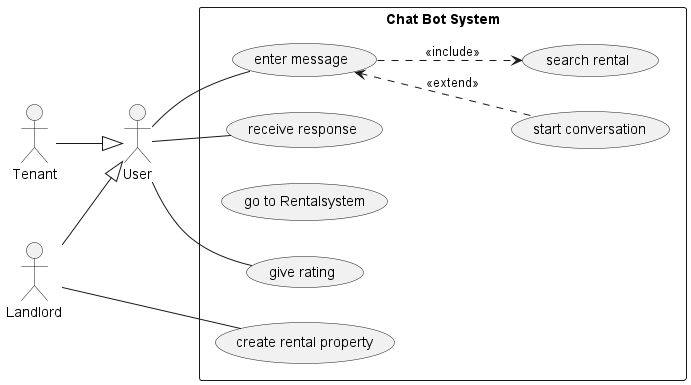
\includegraphics[width = \textwidth]{Images/chat_bot.png}
    \caption{Use Case diagram: AI chat-bot System}
    \label{fig:usecase-diagram-AI-system}
\end{figure}

\newpage
\subsubsection{Use case scenario}
\begin{table}[H]
    \centering
% \usepackage{tabularray}
\begin{longtblr}[
  label = none,
  entry = none,
]{
  width = \linewidth,
  colspec = {Q[125]Q[817]},
  hlines,
  vlines,
}
\textbf{Use-case ID}       & UC-11                              \\
\textbf{Use-case Name}     & Ask question     \\
\textbf{Actor(s)}          & User (Primary)                        \\
\textbf{Description}       & User can enter text to ask chat-bot system to search for specific characteristic rental post~~  \\
\textbf{Pre-condition(s)}  & User logged in successfully to the website                    \\
\textbf{Post-condition(s)} & Chat-bot system return closest results or responses               \\
\textbf{Trigger(s)}        & User clicks or focuses on the search input field                   \\
\textbf{Normal flow}       & {1. User inputs question in the chat box\\2. System processes and queries for the answer result\\3. System responses with an answer on the chat area\\4. System asks if the user wants to continue\\5. User wants to end the conversation\\End use case}  \\
\textbf{Alternative flow}  & {Alternative 1: At step 1 - User enter start conversation message instead of finding rental\\~1.1. User inputs start conversation message (e.g. Hello, Hi,...) \\~1.2. System responses with a greeting\\~1.3. System asks for the intent of user\\~1.4. User inputs question about rental finding\\~Continue at step 2 of the normal flow.
\\Alternative 2: At step 5: User want to ask more.
\\~Return to step 1 of the normal flow.~ ~} \\
\textbf{Exception flow}    & {Exception 1: at step 2 - System cannot understand the intent of Tenant, or Tenant enters value out of context of "finding rental" (e.g, "give me a sandwich")\\~Then the
system will ask again for more information with a guide message}
\end{longtblr}
    \caption{Use case scenario: enter message, receive response}
    \label{tab:usecase-scenario-enter-mess-&-resceive-response}
\end{table}


%-------UC-12-------------
\newpage
\begin{table}[H]
    \centering
% \usepackage{tabularray}
\begin{longtblr}[
  label = none,
  entry = none,
]{
  width = \linewidth,
  colspec = {Q[129]Q[813]},
  hlines,
  vlines,
}
\textbf{Use-case ID}       & UC-12                                  \\
\textbf{Use-case Name}     & Send feedback                          \\
\textbf{Actor(s)}          & User                                   \\
\textbf{Description}       & User send feedback after sending message with Chat-bot system                                        \\
\textbf{Pre-condition(s)}  & User sends message with the system and want to end conversation                                            \\
\textbf{Post-condition(s)} & Chat-bot system updates the feedbacks and to the database for future enhancement plan                     \\
\textbf{Trigger(s)}        & User want to end conversation after receiving response from system                                      \\
\textbf{Normal flow}       & {1. System ask if User wants to continue the conversation\\2. User wants to end the conversation\\3. System asks for rating and feedback\\4. User sends feedback\\5. System responses with the "Thank you!" message\\End use case} \\
\textbf{Alternative flow}  & Alternative 1: at step 2 - User enter new message after chat-bot system asks for feedback and rating. Then return to normal flow of~\textbf{\textbf{use-case UC-11}}      \\
\textbf{Exception flow}    & No exception                           \end{longtblr}
    \caption{Use case scenario: Send feedback}
    \label{tab:usecase-scenario-send-feed-back-AI}
\end{table}

%---------UC-13-----------
\newpage
\begin{table}[H]
    \centering
% \usepackage{tabularray}
\begin{longtblr}[
  label = none,
  entry = none,
]{
  width = \linewidth,
  colspec = {Q[148]Q[796]},
  hlines,
  vlines,
}
\textbf{Use-case ID}       & UC-13                            \\
\textbf{Use-case Name}     & Create rental inventory          \\
\textbf{Actor(s)}          & Landlord                          \\
\textbf{Description}       & Landlord can ask the chat-bot system to create rental inventory in the rental system automatically                                                 \\
\textbf{Pre-condition(s)}  & Landlord has logged in successfully                                                  \\
\textbf{Post-condition(s)} & Rental System create a rental post and adds it to the inventory list of landlord~           \\
\textbf{Trigger(s)}        & Landlord enters input field in chat-bot section with intent "create rental post"              \\
\textbf{Normal flow}       & {1. Landlord enter message\\2. Chat-bot system checks the message and get the all the required fields for a rental post from the message\\3. Chat-bot system prompts confirmation message to chat section\\4. Chat-bot system asks the Rental System to create a rental post and add it into inventory list\\5. Rental system routes to the detail page of the new rental property\\End use case} \\
\textbf{Alternative flow}  & {Alternative 1: At step 2 - The message is lack of some important information for a post (e.g, Price, Address, Image,...)\\~1.1 The chat-bot system asks for more information~\\~Return to step 1 in normal flow} \\
\textbf{Exception flow}    & No exception                     \end{longtblr}
    \caption{Use case scenario: Asking Chat-bot system to create rental property post}
    \label{tab:usecase-scenario-ask-chat-bot-create-rental}
\end{table}




\newpage
\section{Activity Diagrams}
From the use case scenarios, we can imagine the interaction flows between User and the System. But there are some constraints and requirements that we need to specify during the interaction processes between user and the application system, and these constraints can be demonstrated with the activity diagrams.
\subsection{Rental system: Authentication and Authorization}
Firstly, about Authentication and Authorization, there are several features that requires user account to use them. Moreover, because this is an application with goals are to recommend end-user their desire rentals and to connect with the rental owner, we need some validated and trustworthy contact information from the user, the solution is to ask the user to enter their phone number and email when signing up. If not, user can only access to some basic features of the system as guess, we made a table to show which feature user can access with or without an account:

\begin{table}[H]
    \centering
% \usepackage{tabularray}
\begin{longtblr}[
  label = none,
  entry = none,
]{
  width = 0.9\linewidth,
  colspec = {Q[115]Q[462]Q[200]Q[163]},
  row{1} = {c},
  cell{2}{1} = {r=8}{},
  cell{2}{3} = {c},
  cell{2}{4} = {c},
  cell{3}{3} = {c},
  cell{3}{4} = {c},
  cell{4}{3} = {c},
  cell{4}{4} = {c},
  cell{5}{3} = {c},
  cell{5}{4} = {c},
  cell{6}{3} = {c},
  cell{6}{4} = {c},
  cell{7}{3} = {c},
  cell{7}{4} = {c},
  cell{8}{3} = {c},
  cell{8}{4} = {c},
  cell{9}{4} = {c},
  cell{10}{1} = {c},
  cell{10}{3} = {c},
  cell{10}{4} = {c},
  vlines,
  hline{1-2,11} = {-}{},
  hline{3-10} = {2-4}{},
}
                  & \textbf{Feature}                           & \textbf{Without account} & \textbf{With account} \\
\textbf{Tenant }  & View rentals                               & \checkmark               & \checkmark            \\
                  & View rental details                        & \checkmark               & \checkmark            \\
                  & Search rental                              & \checkmark               & \checkmark            \\
                  & Compare 2 rentals                          & \checkmark               & \checkmark            \\
                  & Send message to Landlord                   &                          & \checkmark            \\
                  & Add rental to favorite/saved list          &                          & \checkmark            \\
                  & View saved list                            &                          & \checkmark            \\
                  & Give feedback                              &                          & \checkmark            \\
\textbf{Landlord} & * Every features in Landlord use case view &                          & \checkmark            
\end{longtblr}
    \caption{Accessing features with and without account}
    \label{tab:access-features}
\end{table}

\newpage
By this specification, we present the activity diagrams for Sign-up and Log-in as follow. The goals is to validated the user phone number and email to ensure the credibility of Landlord and communication between end-users.
\begin{figure}[H]
    \centering
    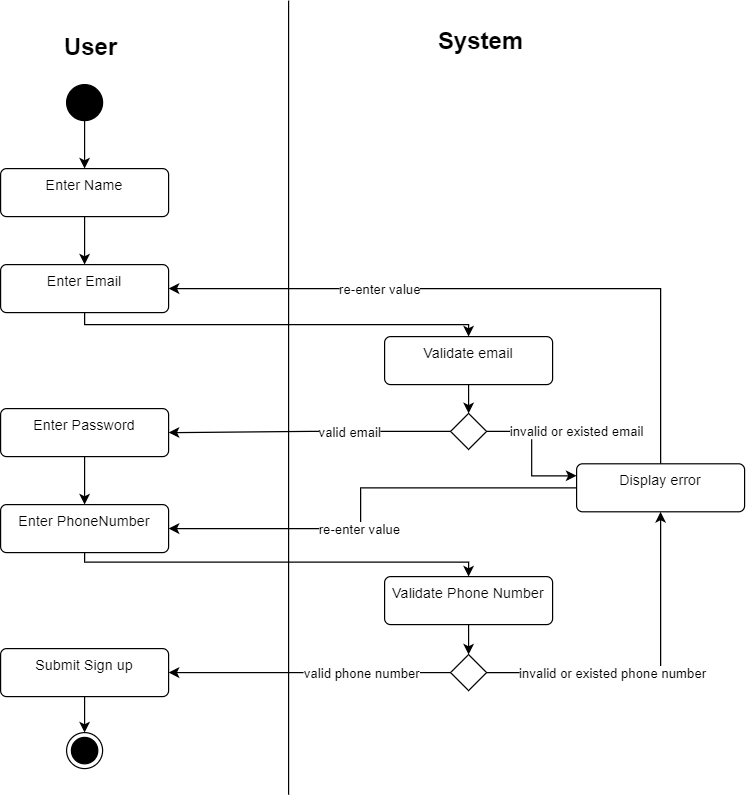
\includegraphics[width = 0.5\textwidth]{Images/Activity/ac_diag_signup.png}
    \caption{Activity diagram: Sign-up flow}
    \label{fig:signup-flow}
\end{figure}

\begin{figure}[H]
    \centering
    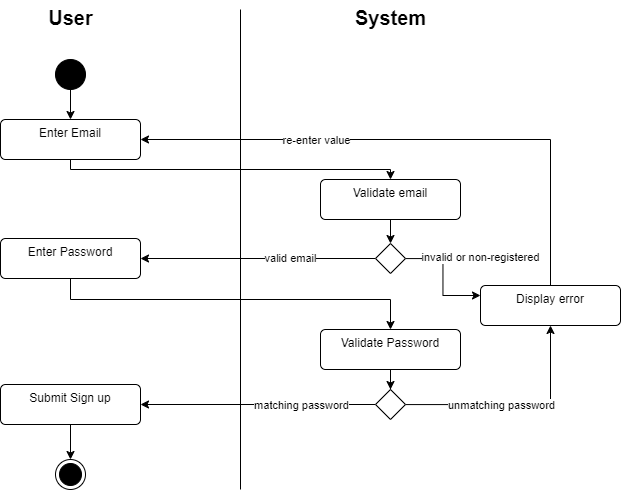
\includegraphics[width = 0.5\textwidth]{Images/Activity/ac_diag_login.png}
    \caption{Activity diagram: Log-in flow}
    \label{fig:login-flow}
\end{figure}

% ------AC_DIAG: TENANT-INTERACTION-------------
\newpage
\subsection{Rental system: Tenant interactions}
Secondly, about Tenant Module, there aren't many restrictions or constraints on the interaction between the Tenant and Rental system, the activity diagram are simply demonstrated the flow of interaction between the user and the system in general.

% -----AC-DIAG_VIew rental-------------
\subsubsection{Viewing the rentals on Tenant landing page or rental detail information page}
\begin{figure}[H]
    \centering
    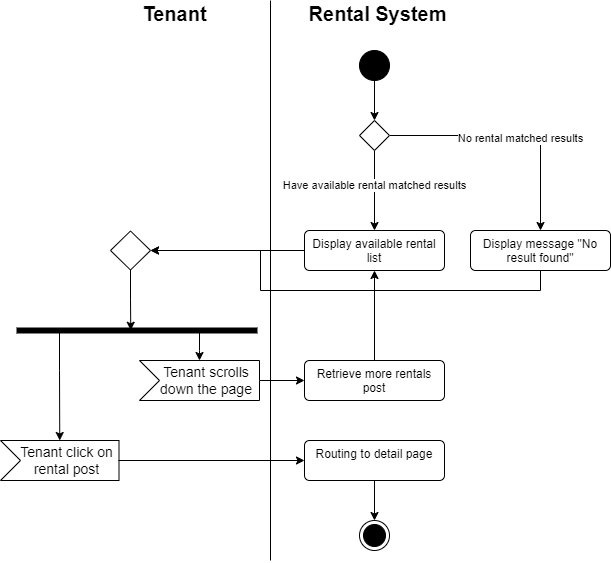
\includegraphics[width = 0.7\textwidth]{Images/Activity/ac_diag_view_rental.png}
    \caption{Activity diagram: Viewing rentals flow }
    \label{fig:ac_diag_view_rental}
\end{figure}

\noindent \textbf{Explanation:}\\
The activity diagram shows the flow when the user access to the website. First page of the website is the Landing page in Tenant view, so the user will be in the role of the Tenant who is looking for a house or an apartment for rent. The system retrieves the latest available rental system and display them with general rental detail to the Tenant.\\
There are two flows that the Tenant can follow. If the Tenant keeps scrolling down for more rentals, then the Rental system will retrieve for more rentals and display them to the page. If the Tenant clicks on a rental post - meaning he/she want to see more detail information about that rental, then the System will retrieve the detail information and redirect the Tenant to the Detail Information page


% -----AC-DIAG_comparing rental-------------
\newpage
\subsubsection{Comparing 2 rentals}
\begin{figure}[H]
    \centering
    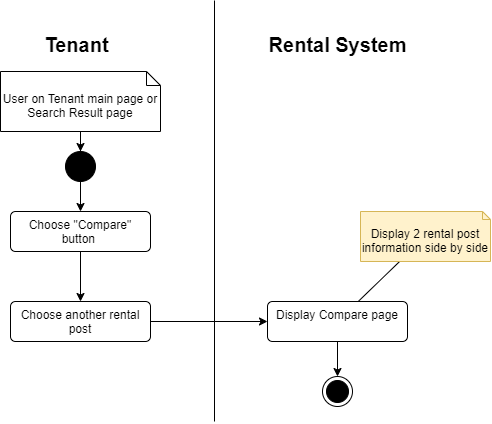
\includegraphics[width=0.8\textwidth]{Images/Activity/ac_diag_compare_2_rentals.png}
    \caption{Activity diagram: Comparing rentals flow}
    \label{fig:compare-rentals}
\end{figure}
\noindent \textbf{Explanation:}\\
The activity diagram describes the flow when the Tenant want to compare 2 rental post. The Tenant is viewing the list of available rentals, he/she can clicking on "Comparison" button on a rental post in the list. The next step is that the System will ask the Tenant to choose another post. Then the Tenant choose another post for starting the comparison or he/she can cancel the comparison process (if the Tenant hit on "Cancel" button, the System will stop asking for the second rental post and let the Tenant continue the Viewing rentals flow). After getting 2 rentals, the System will redirect to the comparison page and display the detail information side by side.


% -----AC-DIAG_searching rental-------------
\subsubsection{Searching rentals}
\begin{figure}[H]
    \centering
    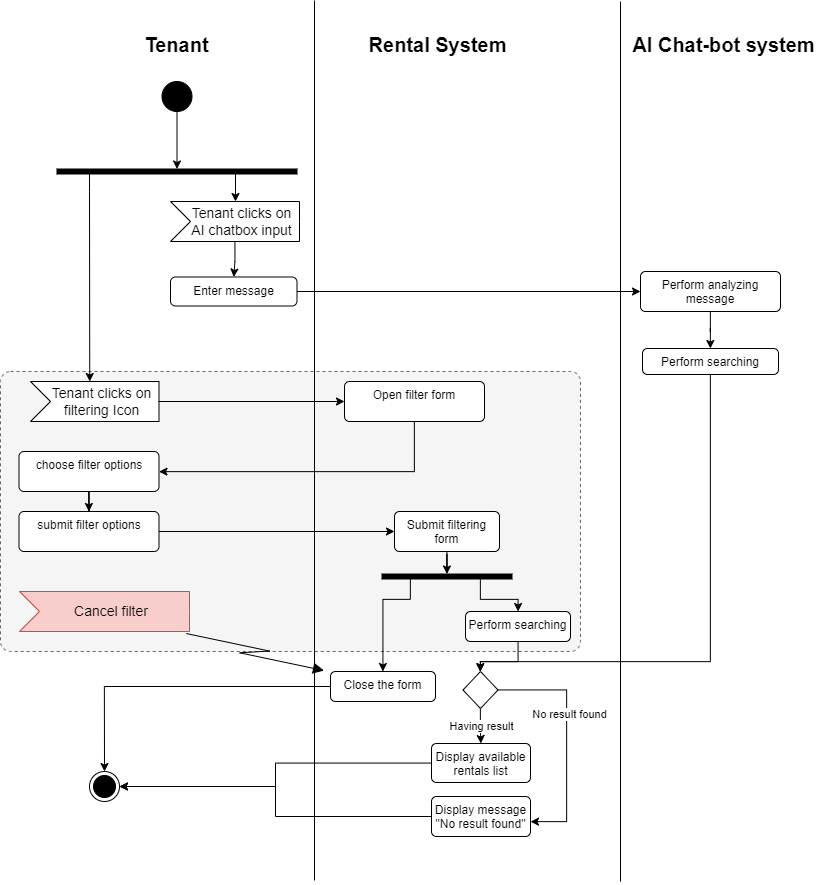
\includegraphics[width=0.7\textwidth]{Images/Activity/ac_diag_search_rental.png}
    \caption{Activity diagram: Searching rentals}
    \label{fig:searching-rentals}
\end{figure}
\noindent \textbf{Explanation:}\\
The activity diagram describes the flows when the Tenant want to search for the rentals based on their criteria. There are 2 ways to help the Tenant achieving their goal: by entering message or by opening the filter.\\
If the Tenant chooses to search by filtering, the System then opens a filtering form so that the Tenant can click and choose the criteria he/she wants (e.g, Property Type, Price Range, Number of rooms, Dimensions,...). Then after the Tenant done choosing and hit the "Save" button, the System can perform searching for the rentals and display the result to the Tenant.\\
If the Tenant chooses to search by entering message, he/she can just enter a message into search input, then a dialog box will be opened and the System can use the Chat-bot AI system to help parsing the message, getting the intent and also the criteria from the user. Then the System performs searching and display the result to the user.


% -----AC-DIAG_adding rental to favorite lsit-------------
\newpage
\subsubsection{Adding rental to favorite list}
\begin{figure}[H]
    \centering
    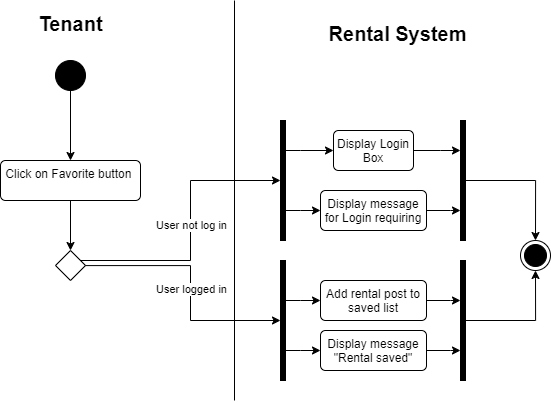
\includegraphics[width=0.8\textwidth]{Images/Activity/ac_diag_add_favorite.png}
    \caption{Activity Diagram: Adding to favorite list}
    \label{fig:add-favorite}
\end{figure}
\noindent \textbf{Explanation:}\\
The activity diagram describes the flows when user saves the rental to his/her favorite list for the later reviewing. The Tenant can click on the "Favorite" button which means he/she want the system to add this rental post into the favorite list. As we mentioned earlier, this feature can only be accessed when User has an account on the website. Therefore, when clicking on the "Favorite" button, the System will perform checking if the User had accessed to the website by Guess account or by his/her account. Then there are 2 case might happen.\\
If the Tenant uses the Guess account, the System displays a Log-In Box with a message, telling the Tenant that they might want to login to use this feature.\\
If the Tenant uses his/her account, the System will perform adding the rental to the favorite list of that account. After adding the post, the System displays a confirmation message to the Tenant 



% _____LANDLORD INTERACTION_____________
\newpage
\subsection{Rental system: Landlord interactions}
Thirdly, about Landlord Module, this allows the User to create, update, delete their rentals inventories. Because the goal is to check and maintain the reliability and the trustworthiness of the rentals and the house owners, these features require the User to log in the website so that they can use them. 
% ----AC_Diag: View rentals-----------
\subsubsection{Viewing rental inventories}
\begin{figure}[H]
    \centering
    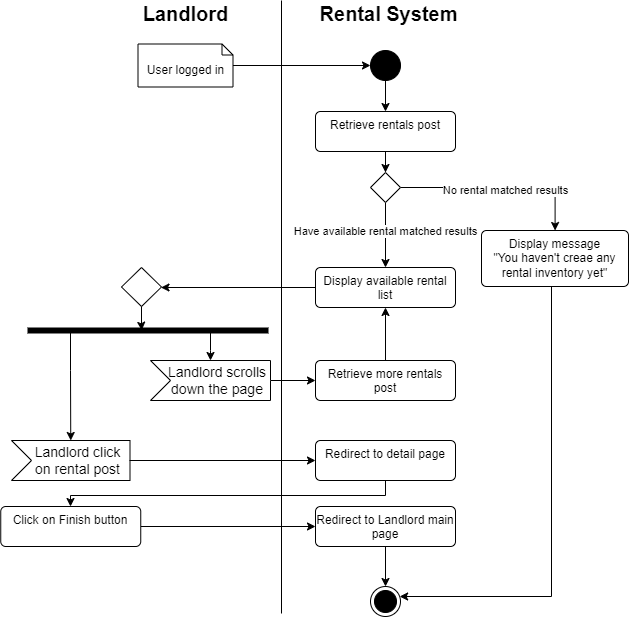
\includegraphics[width=0.9 
    \textwidth]{Images/Activity/ac_diag_view_landlord.png}
    \caption{Activity diagram: Viewing rental inventories}
    \label{fig:viewing-rental-landlord}
\end{figure}
\noindent \textbf{Explanation:}\\
The activity diagram describes the flow of viewing the rental properties when the User changes from Tenant View into Landlord view. When the User clicks on "Landlord" button, he/she will be redirected to Landlord Landing page. The system will retrieve all rental inventories (the rental post that the Landlord had created) and display it on the page. If the Landlord haven't create any rental inventory, the system will display the message onto the page. \\
There are 2 flow that the Landlord can follow. If the Landlord keeps scrolling down for more rentals, then the Rental system will retrieve for more rental inventories and display them to the page from the newest to the oldest rental creation date. If the Landlord clicks on a rental post - meaning he/she want to see more detail information about that rental, then the System will retrieve the detail information and redirect the Tenant to the Detail Information page. After done viewing the detail information, the Landlord can click on "Return" button to return to the Landlord Landing page. 


% -----AC_Diag: Create rental---------
\newpage
\subsubsection{Creating rental inventory}
\begin{figure}[H]
    \centering
    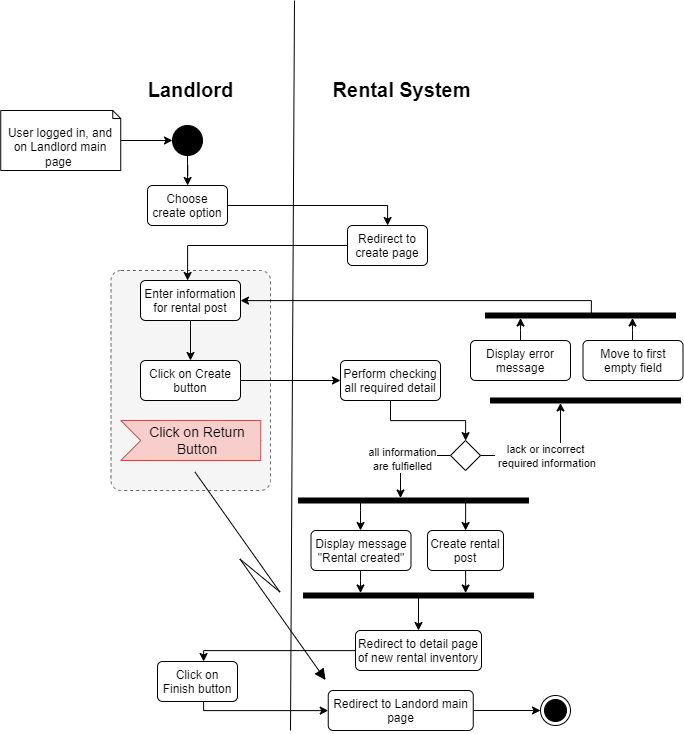
\includegraphics[width=0.7\textwidth]{Images/Activity/ac_diag_create_rental_post_manual.png}
    \caption{Activity diagram: Creating rental property}
    \label{fig:create-rental}
\end{figure}
\noindent \textbf{Explanation:}\\
The activity diagram describes the flow when the Landlord creates a new rental inventory. The system will then redirect the Landlord to the Create page. Then the Landlord can start adding information for his rental inventory.\\
The Landlord can cancel the creating process anytime by clicking on the "Return" button. Then, the System will return on the Landlord Landing page.\\
Because we must keep a rental post reliable, there are some information that is required (address, price, image, owner's phone number)  After the Landlord hit on the "Create" button, the System will check if all required information are fulfilled. If not, the System will display an alert and jump to the information that is invalid for the re-entering. If all information are fulfilled, the System can create a rental post and then redirect the Landlord to the rental detail page of the new rental inventory.

%-------Ac-diag: Update rental--------
\newpage
\subsubsection{Updating rental property}
\begin{figure}[H]
    \centering
    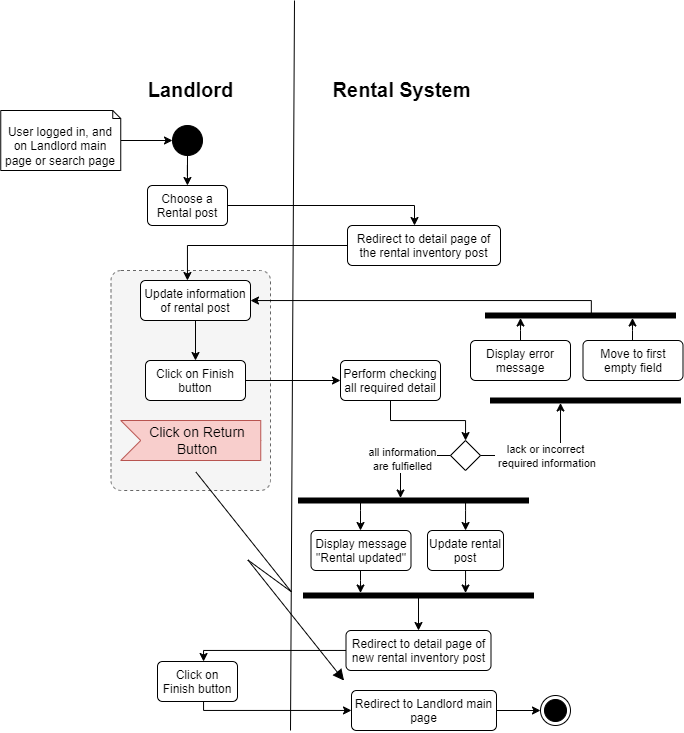
\includegraphics[width=0.7\textwidth]{Images/Activity/ac_diag_update_rental.png}
    \caption{Activity diagram: Updating rental property}
    \label{fig:update-rental}
\end{figure}
\noindent \textbf{Explanation:}\\
The activity diagram describes the flow when the Landlord updates an existing rental inventory. This flow is the same as the "Creating rental inventory flow" but instead of clicking the "Create" button, the Landlord will choose a post in the rental inventory list in Landing page. The system will open the Detail information page of that rental post and the Landlord can start updating the information. The information checking flow and cancelling is almost the same as the "Creating" flow. The system still has to check and ensure that there is no rental information is invalid.


%-------Ac-diag: Delete rental--------
\newpage
\subsubsection{Deleting rental property}
\begin{figure}[H]
    \centering
    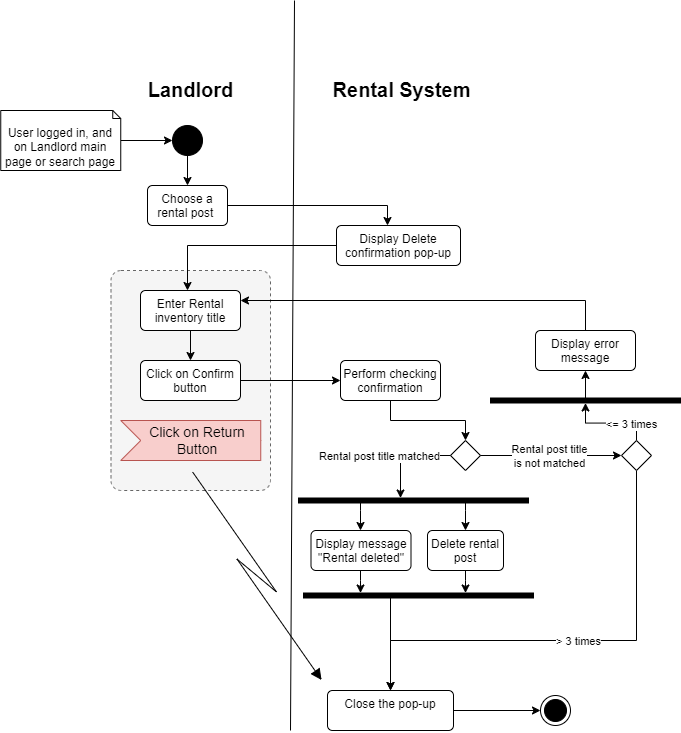
\includegraphics[width=0.7\textwidth]{Images/Activity/ac_diag_delete_post.png}
    \caption{Activity diagram: Deleting rental property}
    \label{fig:delete-rental}
\end{figure}
\noindent \textbf{Explanation:}\\
The activity diagram describes the flow when the Landlord deletes the rental property. When the Landlord want to delete a rental property, he/she can click on the "Delete" button on the rental post if the User is viewing the rentals list or on the Detail information page of a specific rental post.\\
To ensure that the User does not accidentally delete the rental property, the System will display a pop-up that require the Landlord to enter the title of that rental inventory, and also a confirmation message including the rental title (the purpose is to give the owner of the property have time to reconsidering the deletion, not to make the extra step to make it hard to use). \\
Next, the System start checking if the entered title is matching with the actual title or not. If not, the User has 3 tries to enter the correct title, more than 3 times will cause the System cancel the deletion process. After the Landlord entered the correct value, the System will delete the rental post. \\
Moreover, the Landlord cancel the deletion process at anytime.


\newpage
\subsection{Chat-bot system: User interactions}
Finally, about the Chat-bot AI System, the main purpose of the Chat-bot system is to enhance the experience of the User by improving the searching and creating the rental post.
% -----Ac-Diag: Searching chat-bot--------------------
\subsubsection{Interacting with Tenant}
\begin{figure}[H]
    \centering
    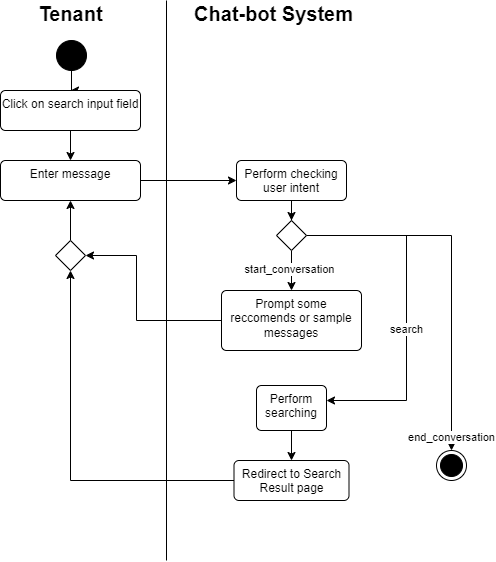
\includegraphics[width=0.9\textwidth]{Images/Activity/ac_diag_search_by_chat_bot.png}
    \caption{Activity diagram: Interaction with Tenant}
    \label{fig:Interaction-with-Tenant}
\end{figure}
\noindent \textbf{Explanation:}\\
The activity diagram describes in more detail the flow when the User search for rental by entering message. The System will receive the message from the User, then it has 3 option to continue the flow.
\begin{itemize}
    \item If the Tenant want to start the conversation, the System will answer with some instruction about how to perform searching with a message.
    \item If the Tenant want to search for rental, the System will get all the criteria from the message and the Rental System will perform searching based on the criteria got from the Chat-bot.
    \item If the Tenant want to end the conversation, the Chat-bot system will display thank you message and ask for the feedback.
\end{itemize}


% -----Ac-Diag: Creating chat-bot--------------------
\newpage
\subsubsection{Interacting with Landlord}
\begin{figure}[H]
    \centering
    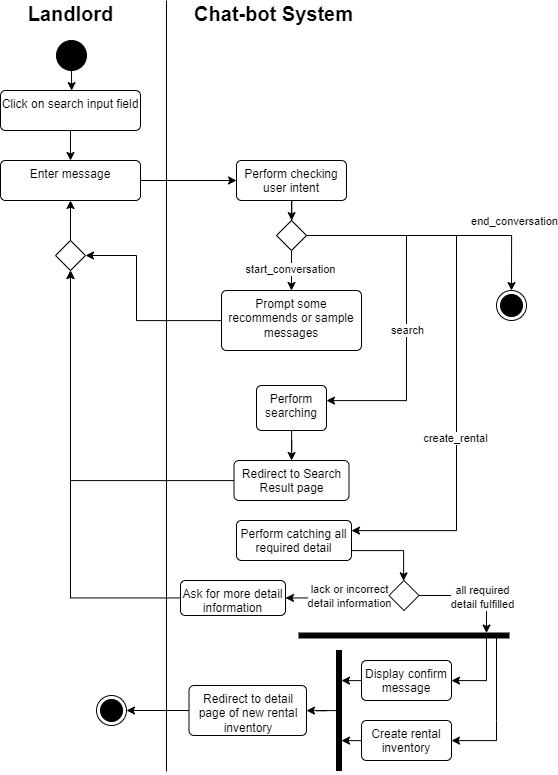
\includegraphics[width=0.8\textwidth]{Images/Activity/ac_diag_create_rental_chat_bot.png}
    \caption{Activity diagram: Interacting with Landlord}
    \label{fig:Interacting-with-Landlord}
\end{figure}
\noindent \textbf{Explanation:}\\
The activity diagram describes in more detail the interaction flow between the Landlord and the Chat-bot system. The System will receive the message from the User, then it has 4 options to continue the flow. There are 3 options that are similar to the interaction flow of the Tenant, but the Landlord interaction has 1 more option which is "Creating rental inventory"\\
\begin{itemize}
    \item If the Landlord want to start the conversation, the System will answer with some instruction about how to perform searching with a message.
    \item If the Landlord want to search for rental, the System will get all the criteria from the message and the Rental System will perform searching based on the criteria got from the Chat-bot and display the result to the Landlord.
    \item If the Landlord want to end the conversation, the Chat-bot system will display thank you message and ask for the feedback.
    \item If the Landlord want to create a new rental inventory, the Chat-bot system will retrieve all information from the message for the new rental inventory. Again, if the required information are not fulfilled, the System need to send the message asking the user to enter more information until it can make a new rental inventory. After the creation process, the Landlord will be redirect to the Detail page of the new rental inventory.
\end{itemize}


% ######### SEQUENCE DIAGRAM ########
\newpage
\section{Sequence diagrams}
\subsection{Tenant Interaction}
\subsubsection{Viewing rental and rental detail}
\begin{figure}[H]
    \centering
    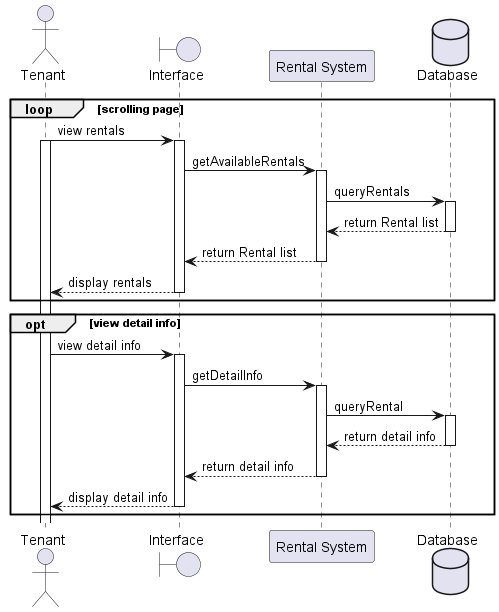
\includegraphics[width=0.7\textwidth]{Images/Sequence/seq_diag_view_rental.png}
    \caption{Sequence diagram: view rental and rental detail}
    \label{fig:seq-diag-view-rental}
\end{figure}
\noindent \textbf{Explanation:}\\
The sequence diagram explains how the Tenant can see the rental on the website. In this context, the Interface in the diagram refers to the User Interface, but we will named it "Interface" for short. When the Tenant is on the Tenant Landing page, the Interface need the list of available rentals to show to the Tenant. Therefore, the Rental System will retrieve rental from the Database. After the Database return the result, the System will display them to the User through the Interface.


\newpage
\subsubsection{Comparing rentals}
\begin{figure}[H]
    \centering
    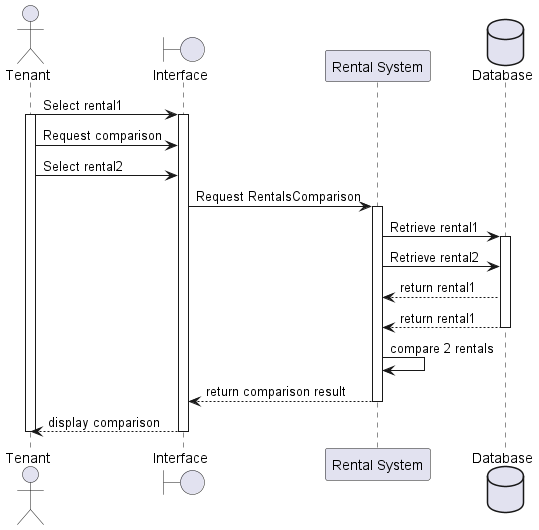
\includegraphics[width=0.8\textwidth]{Images/Sequence/compare_rental.png}
    \caption{Sequence diagram: Comparing 2 rentals}
    \label{fig:seq-diag-compare}
\end{figure}
\noindent \textbf{Explanation:}\\
The sequence diagram shows how the Tenant can compare 2 rentals but the idea of the flow is already described in the activity diagram. After Tenant clicked on the "Compare" button on a rental post and chose the second rental post, this mean it issues the rental comparison feature of the Rental System. The System will based on the 2 chosen rental post to retrieve more information from the Database, then rearranged the information in the way that the Interface can display these detail information side by side to the Tenant. 


\newpage
\subsubsection{Searching rental}
\begin{figure}[H]
    \centering
    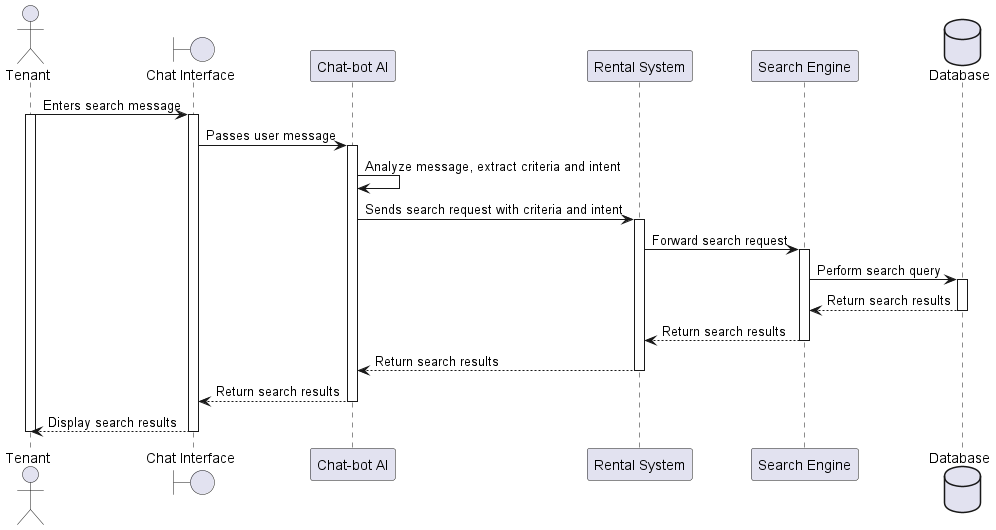
\includegraphics[width=0.9\textwidth]{Images/Sequence/seq_diag_search.png}
    \caption{Sequence diagram: Searching rentals}
    \label{fig:seq-diag-search}
\end{figure}
\noindent \textbf{Explanation:}\\
The sequence diagram describes how the Tenant can perform searching for the rentals. The Tenant enters the message to search through the Interface, and the Chat-bot System is responsible for handling the message. The handling message process includes analyze, extract all criteria and detect the intent from the message, and pass them to the Rental System. Next, the System will use the Search Engine and the information to query form the Database. After the Database returns the result, the Rental System will passed it to the Chat-bot System so it can create a message and responses to the User. 



\newpage
\subsubsection{Saving and viewing favorite list}
\begin{figure}[H]
    \centering
    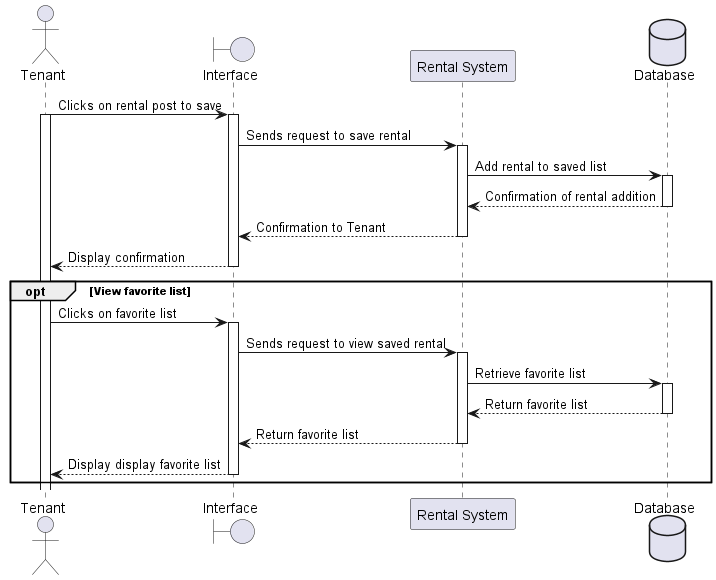
\includegraphics[width=0.8\textwidth]{Images/Sequence/seq_diag_save_&_view_saved_rental.png}
    \caption{Sequence diagram: Saving and viewing favorite list}
    \label{fig:seq-diag-favorite}
\end{figure}
\noindent \textbf{Explanation:}\\
The sequence diagram describe how the Tenant can save and might view the favorite list. The sequence is the same as the flow described in the Activity diagram. When the user clicks on the "Save" button on a rental post, the System can update the rental post to the Database, and then confirm back to the User if success.


\newpage
\subsection{Landlord Interaction}
\subsubsection{Creating rental with the Interface}
\begin{figure}[H]
    \centering
    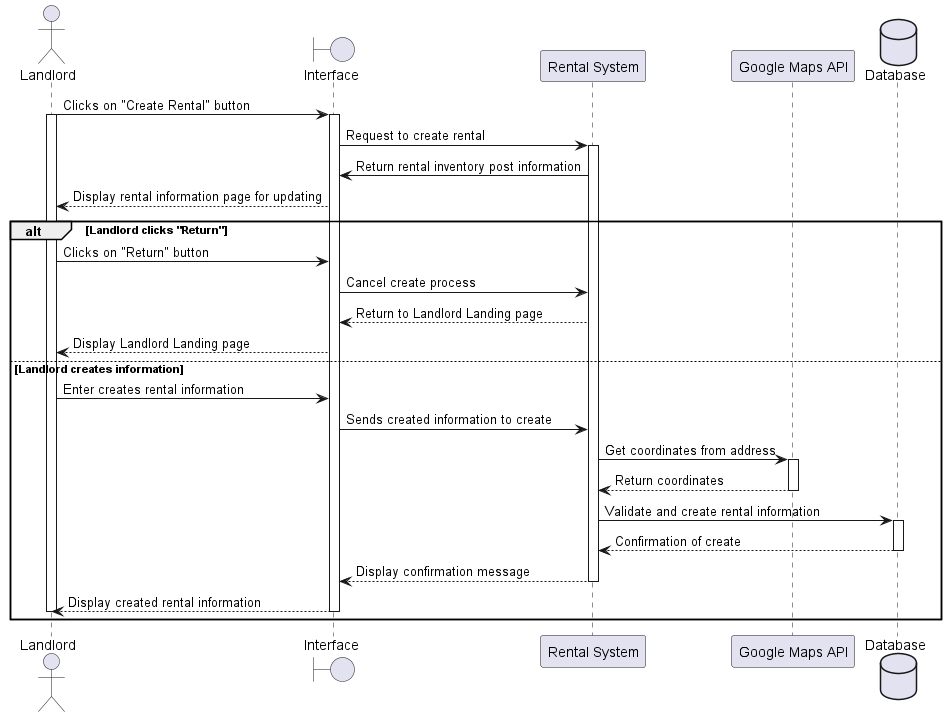
\includegraphics[width=0.9\textwidth]{Images/Sequence/seq_diag_create_rental_inventory.png}
    \caption{Sequence diagram: Creating rental with the Interface}
    \label{fig:seq-diag-create-chat-bot}
\end{figure}
\noindent \textbf{Explanation:}\\
The sequence diagram illustrates how landlord create a new rental inventory. The sequence has the similar flow described in the activity diagram, except there is an extra step before the System tell the Database to create a new rental. Because we need to get the coordinates of the rental for the business logic, the System need to call Google API to get the coordinates from the address, then the System can tell the Database to create a new rental for the Landlord.


\newpage
\subsubsection{Creating rental with Chat-bot system}
\begin{figure}[H]
    \centering
    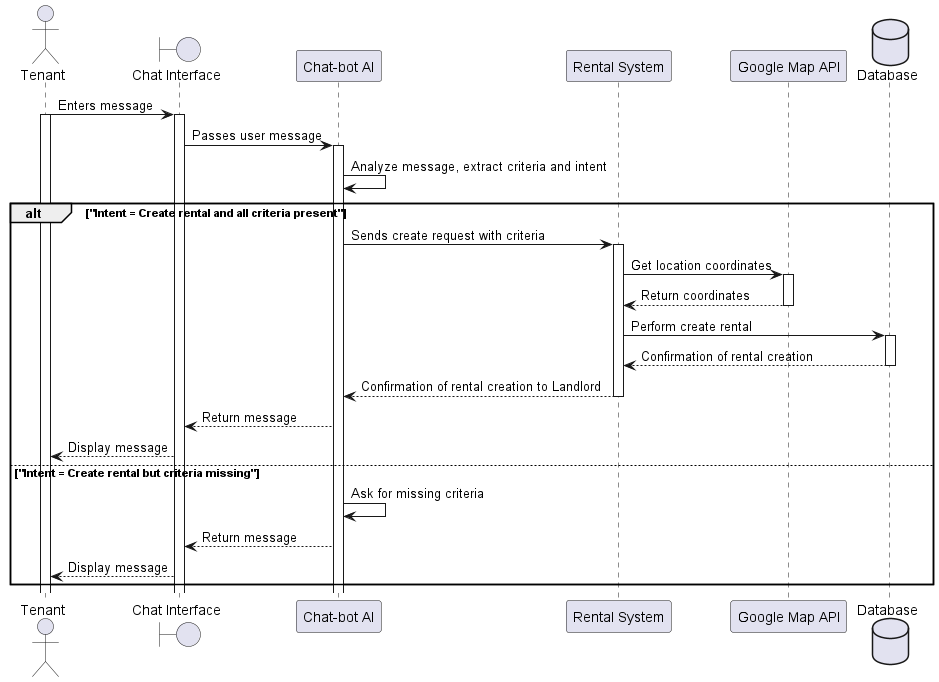
\includegraphics[width=0.9\textwidth]{Images/Sequence/seq_diag_create_rental_inventory_bot.png}
    \caption{Sequence diagram: Creating rental with Chat-bot system}
    \label{fig:seq-diag-create-chat-bot}
\end{figure}
\noindent \textbf{Explanation:}\\
The sequence diagram illustrated how the Landlord can create a new rental inventory, but this time with the help of the Chat-bot system. Instead of entering the information in the fields on the page, the Landlord now enters a message to the Chat-bot so it can analyze the intent of the Landlord and the criteria in the message. If the message does not contains enough information for the creation process than the Chat system can generate the response to ask for more information.
Consequently, if all information are fulfilled then the Chat System can pass them to the Rental System. Here, the next steps is similar to the sequence happened when the Landlord create a new rental with the User Interface.



\newpage
\subsubsection{Updating rental information}
\begin{figure}[H]
    \centering
    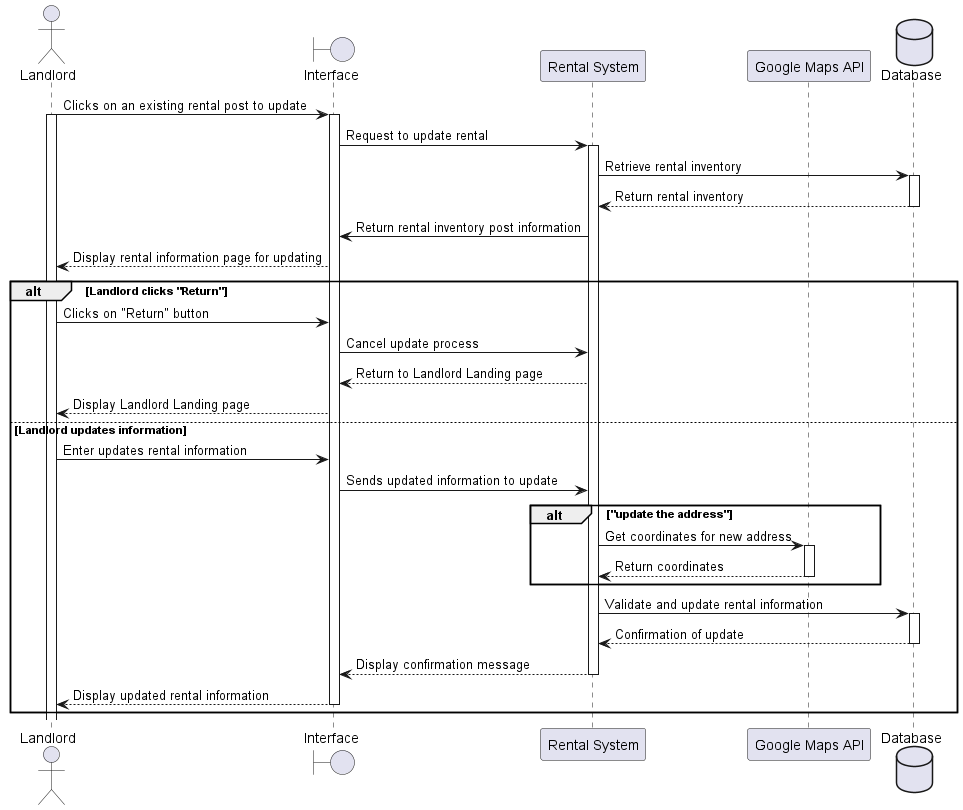
\includegraphics[width=0.9\textwidth]{Images/Sequence/seq_diag_update_rental_inventory.png}
    \caption{Sequence diagram: Updating rental inventory}
    \label{fig:update-rental}
\end{figure}
\noindent \textbf{Explanation:}\\
The sequence diagram describes how the Landlord can update the information of a specific rental inventory. The flow is also described in the activity diagram, this sequence diagram only explains more about the actions of the Rental System when it retrieves and process the detail information from the Database to display to the Landlord; or when the System need to call the API from Google Maps to derive the coordinates of the address of the rental (if the User updates a new address) before it perform updating to the Database.


\newpage
\subsubsection{Deleting rental inventory}
\begin{figure}[H]
    \centering
    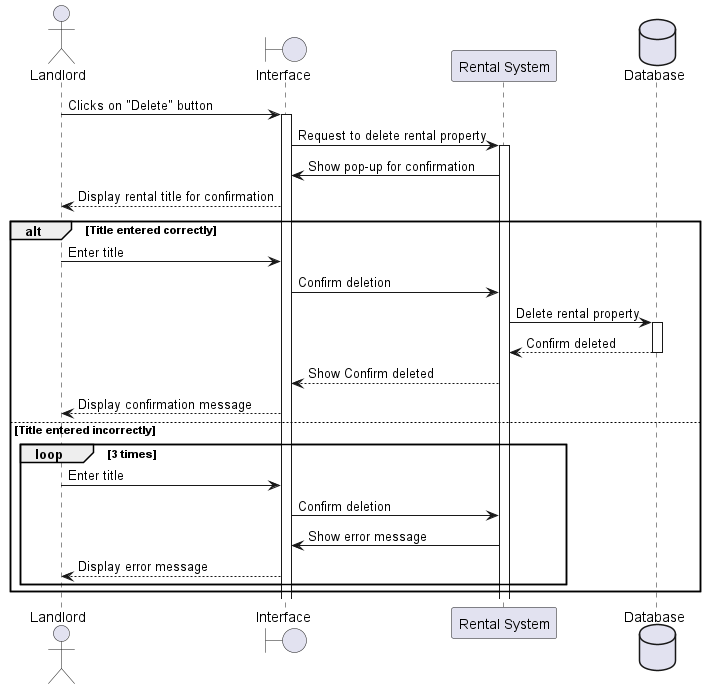
\includegraphics[width=0.8\textwidth]{Images/Sequence/seq_diag_delete_rental_inventory.png}
    \caption{Caption}
    \label{fig:enter-label}
\end{figure}
\noindent \textbf{Explanation:}\\
The sequence diagram illustrates the message exchanged when the Landlord deletes an existing rental inventory. This flow is also similar to the flow described in the corresponding activity diagram. The Landlord click on the "Delete" button when he/she decides to delete this rental. This event issue the Rental System to open a pop-up that require the User to confirm the deleting. Then, the System can check to confirmation and continue to delete the rental inventory.
\chapter{System modeling}
In this chapter, we focus on describing the System designs. We will start with the general architecture of our system, and then continue to the Intent specification and the Conversation flow for the Chat System. Next, we will describe the system design at the level of classes and interfaces to show their features, constraints and relationships. Our database design and mock-up design will also be reported.
\section{General Architecture}
\begin{figure}[H]
    \centering
    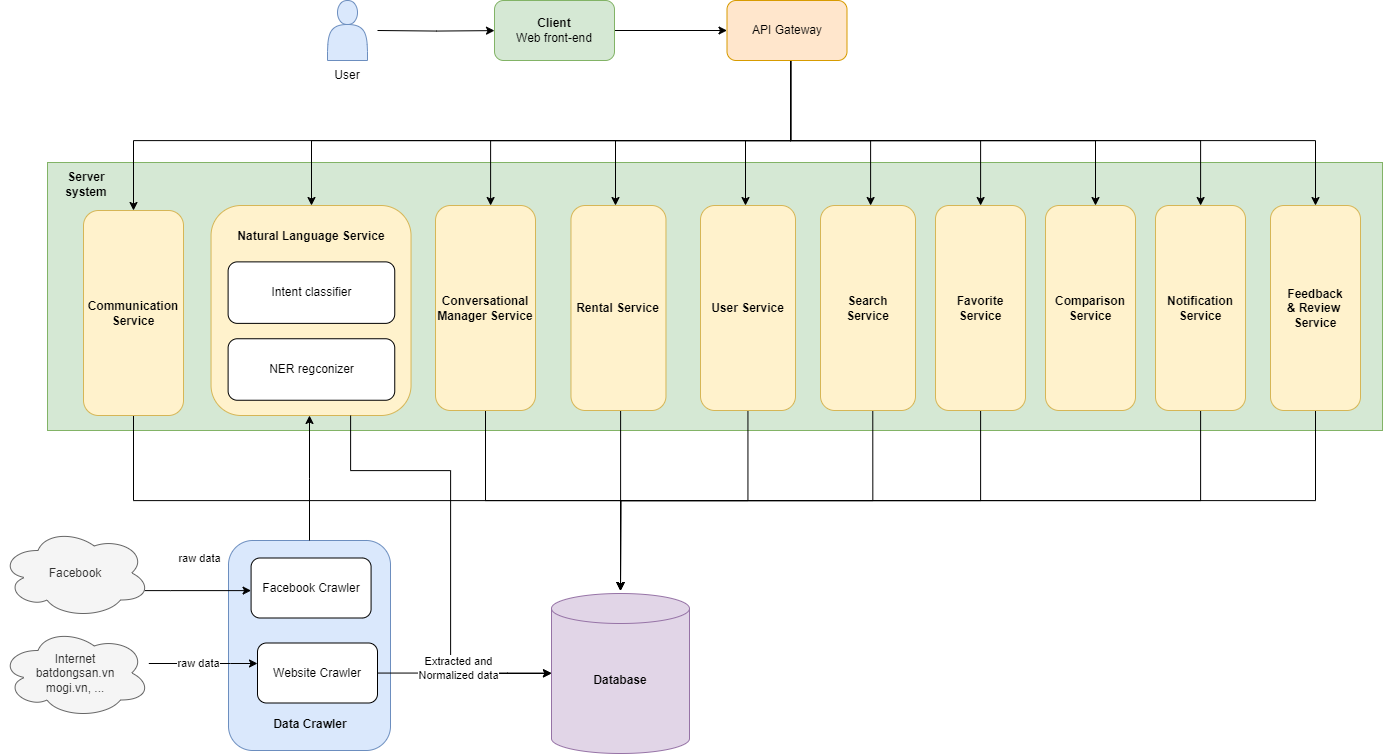
\includegraphics[width=\textwidth]{Images/System_architecture.png}
    \caption{System design: system architecture}
    \label{fig:sys-architect}
\end{figure}
Regarding the system's architectural approach, we are considering a combination of client-server architecture and micro-services in the server. The client-side, which provides the user interface to interact with the System, can be accessed by the User like a web application on a personal computer. On the server side, we break the system down into multiple modular and independent services. The server of the system contains 5 Microservices:
\begin{itemize}
    \item \textbf{Natural Language Service:} classify the intent and recognize the Name entities to catch the criteria in the User's message.
    \item \textbf{Conversational Manager Service:} control the conversational flow and generates a response to the User.
    \item \textbf{Rental Service:} manage the rental properties.
    \item \textbf{User Service:} manage user's account.
    \item \textbf{Search Service:} responsible for the rental searching request from the User.
    \item \textbf{Favorite Service:} provides functionality for users to save, organize, and interact with their favorite rental within the system.
    \item \textbf{Comparison Service:} responsible for the comparison 2 rental feature 
    \item \textbf{Notification Service:} Manage and deliver notifications according to the event. The events could be new messages incoming, updates on favorite rentals, ...
    \item \textbf{Communication Service:} responsible for communication and chatting between users.
\end{itemize}

Furthermore, we also decided to implement an API Gateway. The API Gateway is like an intermediary, functioning as the only entry point to our microservices system. It takes in requests from the client, performs necessary modifications, authenticates them, and then directs these requests to specific APIs within the backend services.

In addition, we decided to use a shared database for our system in this phase. The purpose of using a shared Database is to simplify schema management and to make data retrieval more efficient since all relevant information is stored in a centralized database, services can access the necessary data without the need for complex communication protocols.

\section{Intent specification}
We define the intents of our system as follows:

\subsection{Search intent}
\textbf{Description}: The intent Search is triggered when the user wants to search for the accommodations. The user can provide the location, price, area, or other criteria to search for the accommodations. 

\noindent \textbf{Example}: Some examples of the Search intent are shown below:
\begin{itemize}
    \item "Tôi muốn tìm phòng trọ quận 10, gần đại học Bách Khoa" (I want to find a room in district 10, near Bach Khoa University)
    \item "Tôi muốn tìm phòng trọ giá dưới 2 triệu" (I want to find a room with the price under 2 million VND)
\end{itemize} 

\noindent \textbf{Expected response}: The chatbot will return a list of rental posts that match the user's preferences.

\subsection{Post intent}
\textbf{Description}: The Post intent is triggered when the landlord wants to post their room for rent. Same with the Search intent, the user can provide some additional information such as the location, price, area, or other criteria. 

\noindent \textbf{Example} Some examples of the Post intent are:
\begin{itemize}
    \item "Tôi có phòng trọ trống tại quận 10, cần cho thuê với giá 2 triệu" (I have a room for rent in district 10 with the price of 2 million VND)
    \item "Tôi muốn đăng phòng trọ ở quận 10, gần đại học Bách Khoa" (I want to post a room in district 10, near Bach Khoa University)
\end{itemize}

\noindent \textbf{Expected response}: The chatbot will ask the landlord to provide more required information about the room such as the price, location, and area, ... Then the chatbot will post the room on the website.

\subsection{Provide information intent}
\textbf{Description}: The Provide information intent is triggered when the user answers the chatbot's question. 

\noindent \textbf{Example}: Some examples of the Provide information intent are:
\begin{itemize}
    \item Chatbot: "Bạn cần tìm phòng trọ ở đâu?" (Where do you want to find a room?). User: "Quận 10" (District 10)
    \item Chatbot: "Bạn cần tìm phòng trọ giá khoảng bao nhiêu?" (What is your budget?). User: "Dưới 2 triệu" (Under 2 million)
\end{itemize}

\noindent \textbf{Expected response}: The chatbot will store the information provided by the user for later actions.

\subsection{Other intents}
Besides the main intents above, we also define some other intents such as Greeting, Confirm, Reject, and Fallback that support the process of getting information from the user. 

{\renewcommand{\arraystretch}{1.75}%
\begin{table}[ht]
    \centering
    \begin{tabular}{|l|l|}
        \hline
        \textbf{Intent} & \textbf{Description} \\ \hline
        Greeting & Users want to greet the chatbot and start the conversation. \\ \hline
        Confirm & Users confirm the information that the chatbot responds to. \\ \hline
        Reject & Users reject the information that the chatbot responds to. \\ \hline
        Fallback & Triggered when the user's message does not match any of the intents above.  \\ \hline
    \end{tabular}
\end{table}}

\section{Entities Specifications}
In this section, we define the entities of our system in Figure \ref{fig:entities} and the specifications in Table \ref{tab:entities-specifications}.

\begin{figure}[ht]
    \centering
    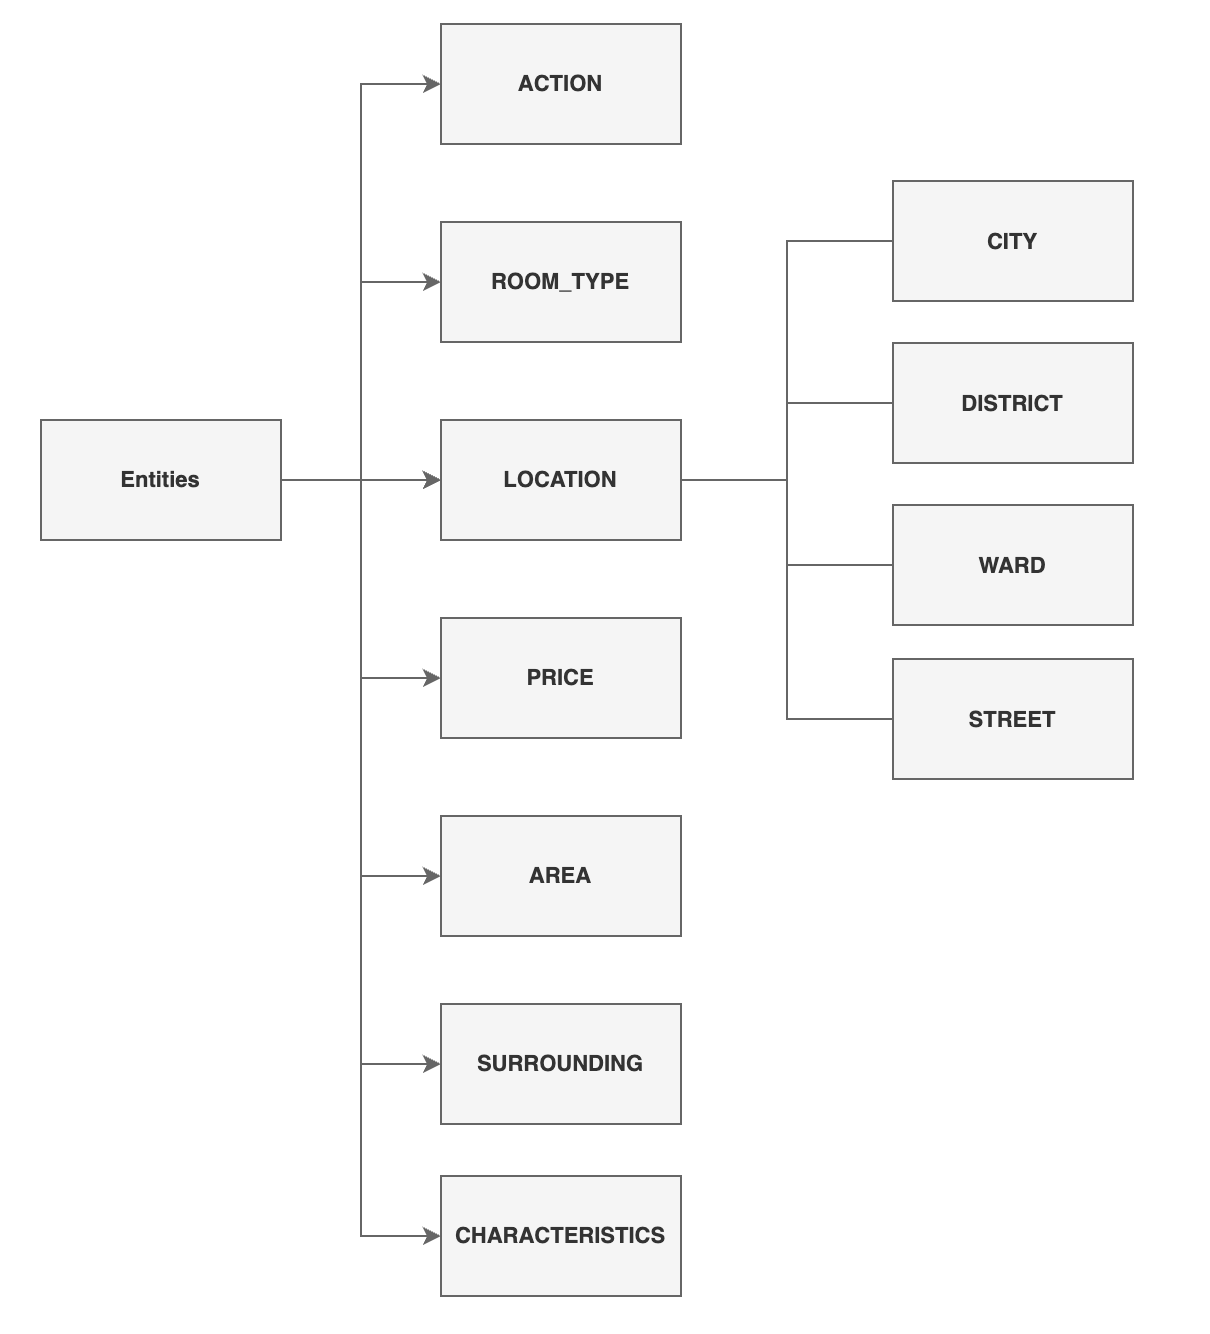
\includegraphics[width=0.8\textwidth]{../Images/7.System_Modeling/entities.png}
    \caption{Entities of the system}
    \label{fig:entities}
\end{figure}

{\renewcommand{\arraystretch}{1.75}%
\begin{table}[ht]
    \centering
    \begin{tabular}{|l|l|}
        \hline
        \textbf{Entites} & \textbf{Description} \\ \hline
        ACTION & The action that users want. Ex: tìm phòng (search) or cho thuê phòng (post). \\ \hline
        ROOM\_TYPE & The type of the room. Ex: phòng trọ (room for rent), chung cư (apartment),... \\ \hline
        CITY & The city name where the room is located. \\ \hline
        DISTRICT & The district name. Ex: quận 10 (district 10) \\ \hline
        WARD & The ward name. Ex: phường 14 (ward 14) \\ \hline
        STREET & The street name. Ex: đường Lý Thường Kiệt (Ly Thuong Kiet street)\\ \hline
        PRICE & The price of the room. Ex: 2 triệu, 2tr (2 million VND) \\ \hline
        AREA & The area of the room. Ex: 20m2, 20 mét vuông (20 square meters) \\ \hline
        SURROUNDING & The surrounding of the room (university, hospital,...)\\ \hline
        CHARACTERISTICS & The characteristics of the room. Ex: yên tĩnh, có chỗ để xe (has parking lot) \\ \hline

    \end{tabular}
    \caption{Entities specifications}
    \label{tab:entities-specifications}
\end{table}}
\clearpage

\section{Conversational Flow}

We have defined 2 main conversational flows for our system. The first flow is for the user to search for rental posts. The second flow is for the landlord to post their room for rent. The system conversational flow is shown in Figure \ref{fig:conversational-flow}.

\begin{figure}[ht]
    \centering
    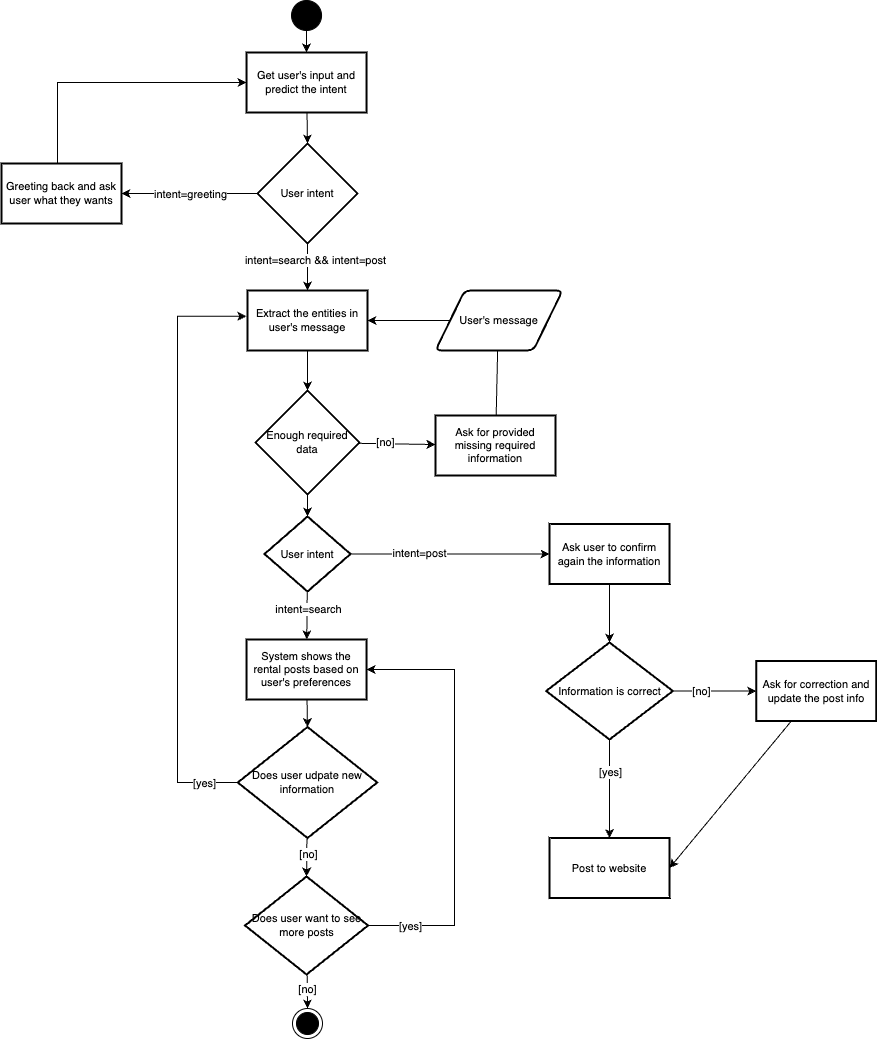
\includegraphics[width=0.8\textwidth]{../Images/7.System_Modeling/conversational_flow.png}
    \caption{The system conversational flow}
    \label{fig:conversational-flow}
\end{figure}

\section{Intent Classification Model}
\label{sec:intent-classification-model}
To implement the Intent Classification Model, we choose to follow the BERT feature-based approach. We use PhoBERT as the pre-trained language model to create word embedding vectors for the input. After that, the word embedding is fed into a fully connected neural network with the softmax layer to classify the intent. The model architecture is shown in Figure

\begin{figure}[ht]
    \centering
    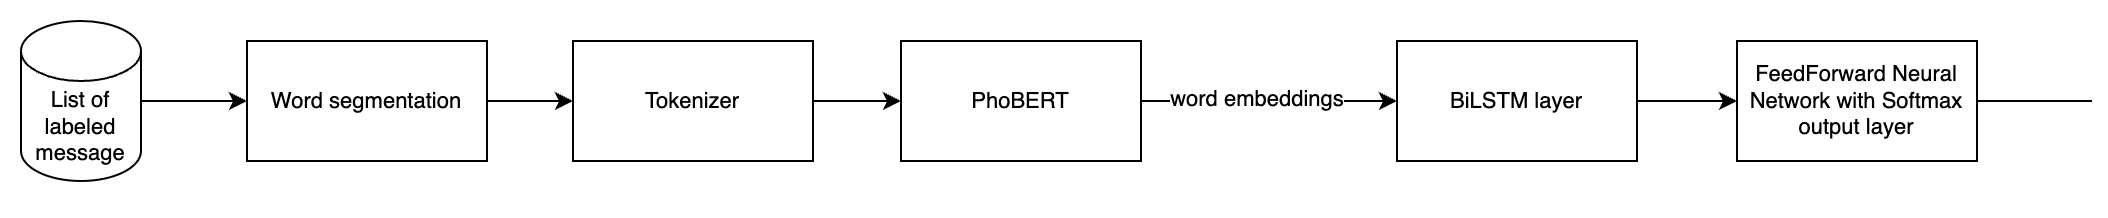
\includegraphics[width=\textwidth]{../Images/7.System_Modeling/intent_classifier_architecture.png}
    \caption{The architecture of Intent Classification Model}
    \label{fig:intent-classification-model}
\end{figure}

PhoBERT is trained on a large corpus of the Vietnamese language, so it can help our model have the general knowledge about the Vietnamese knowledge. Then we train the BiLSTM layer with the Fully Connected layer on the intent classification dataset, which allows the model to get the domain-specific knowledge and learn the pattern for the intent classification task. Our system has a total of 7 intents, so the output of the softmax layer is a vector of 7 elements. The element with the highest value is the predicted intent. 

\section{Named Entity Recognition Model}
We continue to use the PhoBERT feature-based approach for the Named Entity Recognition Model. The model architecture is shown in Figure \ref{fig:ner-model}.

\begin{figure}[ht]
    \centering
    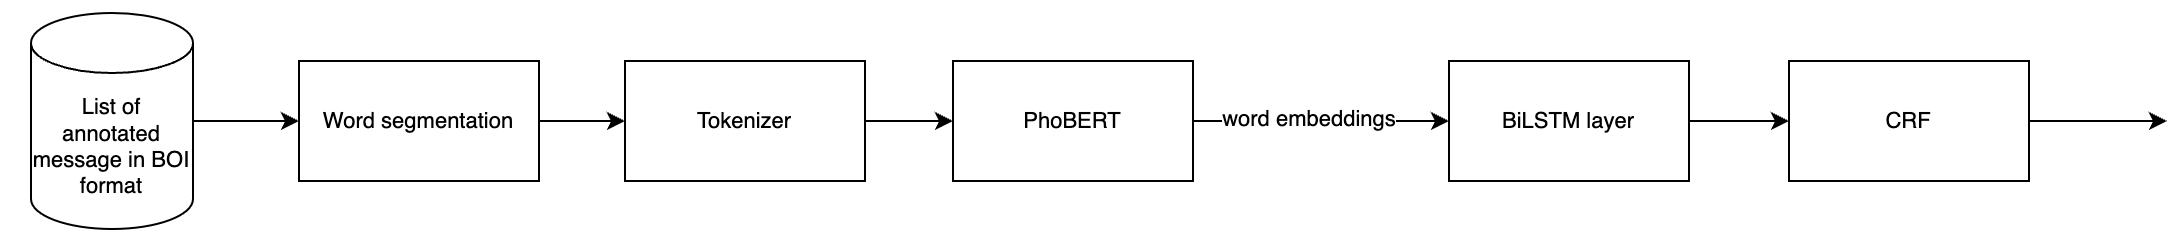
\includegraphics[width=\textwidth]{../Images/7.System_Modeling/ner_architecture.png}
    \caption{The architecture of Named Entity Recognition Model}
    \label{fig:ner-model}
\end{figure}

To train the NER model, we need the annotated data in the BOI format that we mentioned in Chapter \ref{chap:theoretical-background}. We use the same pre-trained language model for both intent classification and NER. We can combine these two models after training independently. The output of the NER model is the value returned by the CRF (conditional random field) layer. The output of the CRF layer is the same length as the input. Each element of the output is the predicted tag for the corresponding word. The tag is one of the following values: B-ROOM\_TYPE, I-ROOM\_TYPE, B-CITY, I-CITY, B-DISTRICT, I-DISTRICT, B-WARD, I-WARD, B-STREET, I-STREET, B-PRICE, I-PRICE, B-AREA, I-AREA, B-SURROUNDING, I-SURROUNDING, B-CHARACTERISTICS, I-CHARACTERISTICS, O. The tag O means that the word is not an entity. 

% %%%%%% DATABASE DESIGN%%%%%%%%%%%%%%%%%%%%
\newpage
\section{Database Design}
The purpose of this Database is to store information about the user's account, rental post, favorite list, message, and notification. The database schema contains 12 entities, each entity is defined with its attributes. The list of entities and the relationship between these entities can be described using the ERD Diagram. 
\subsection{ERD Model}
\begin{figure}[H]
    \centering
    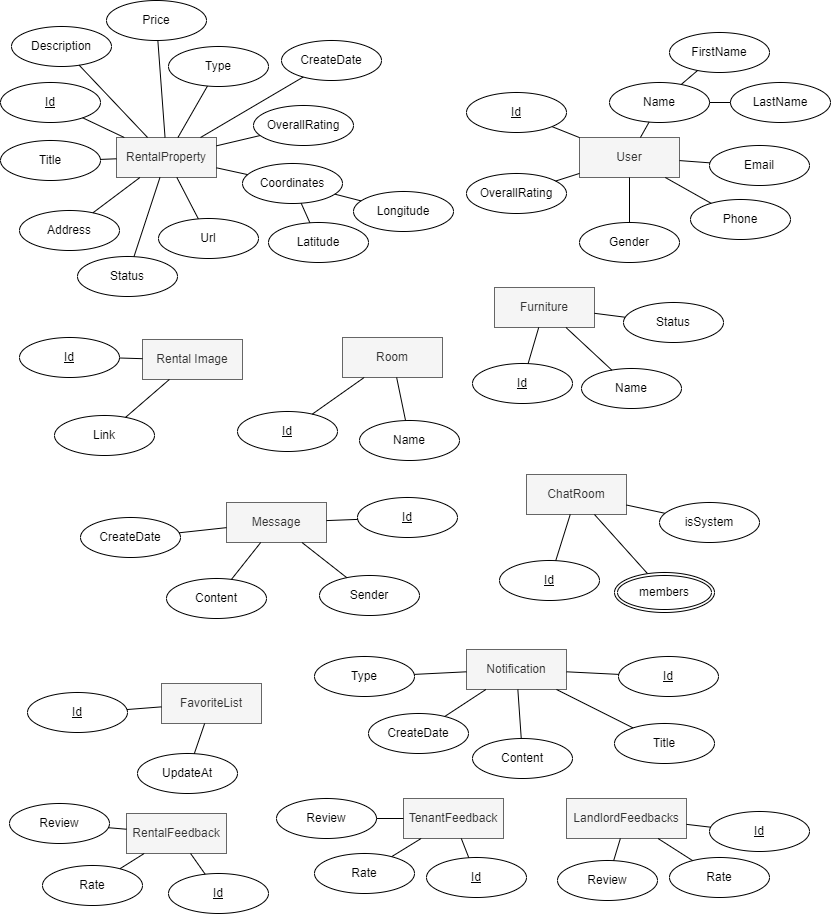
\includegraphics[width=0.85\textwidth]{Images/ERD.png}
    \caption{Database design: List of entities}
    \label{fig:DB-list-entities}
\end{figure}
The database should be able to store data related to the services according to the system architecture. Therefore, firstly we need to list out the entities with their attribute according to the requirement elicitation:
\begin{itemize}
    \item Listing and searching for rental properties
    \item Managing favorite list contains favorite rental
    \item Managing user accounts and profiles
    \item Sending and receiving messages through chats
    \item Sending and receiving notifications about rental properties and other system events
    \item Managing feedback about User and Rental
\end{itemize}

\begin{figure}[H]
    \centering
    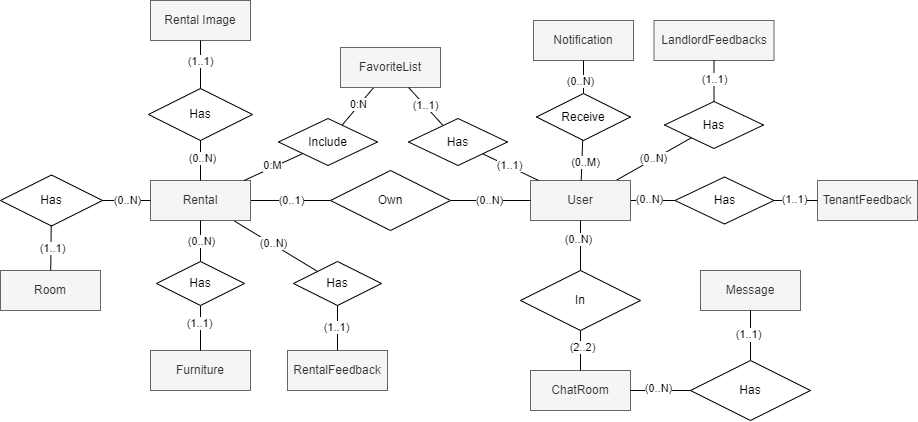
\includegraphics[width=\textwidth]{Images/ERD-Relationship.png}
    \caption{Database design: Entity - Relationship Diagram}
    \label{fig:erd-relationship}
\end{figure}
Next, we need to specify the relationships between these entities. The relationship can be described based on the specifications as follows:
\begin{itemize}
    \item A user can have zero or many rentals, and a rental can be associated with zero or many users (because some rentals might be crawled from the internet)
    \item A user can have zero or many feedback, while feedback must be associated with exactly one user. A user will have 2 view: user as the Tenant and user as the Landlord. By that reason, a User should have 2 type of feedback: Landlord feedback and Tenant feedback.
    \item A rental can have zero or many images, while each image must belong to exactly one rental.
    \item A rental can have zero or many room (bedrooms, living-rooms, bathrooms,...), while each room must belong to exactly one rental.
    \item A rental can have zero or many furniture (washing machine, stove, Wi-Fi, ...), while each furniture must belong to exactly one rental.
    \item A rental will also have zero or multiple feedback, and a rental feedback must also belongs to exactly one rental. 
    \item A user has one favorite rental list, and the list can contains zero or many rental.
    \item A User can receive notifications. Therefore, a user should be associated with multiple notification. Moreover, a notification can be published to multiple user.
    \item A user can join in multiple chat-room, while each chat-room should contains exactly 2 members (user - user or user - chat-bot).
    \item A chat-room also contains multiple messages, while a message must belongs to exactly 1 chat-room. 
\end{itemize}
\section{Mock-up}
\subsection{Tenant User Interface}
\subsection{Landlord User Interface}
\chapter{Technology Stack}

\section{Programming Language}

\subsection{Python}
\textbf{Python} is an easy-to-learn and powerful programming language. It was created by Guido van Rossum. Python is designed to be a general-purpose language, which means that it can be applied in a wide range of domains such as web development, data science, machine learning, etc. In the process of developing the project, our group chose Python 3.11 as the main programming language to build machine learning models and the API server. The reasons for choosing Python are:
\begin{itemize}
    \item Python with clean and simple syntax is easy to learn and use. When developing the application with Python, we can focus on the core idea of the application instead of worrying about the syntax.
    \item Python has a large community and a huge number of libraries, especially in the field of machine learning and web development. Some popular libraries are NumPy, Pandas, Scikit-learn, TensorFlow, PyTorch, etc.
    \item Python is a cross-platform language, which means that it can run on many operating systems such as Windows, Linux, macOS, etc.
\end{itemize}

\begin{figure}[ht]
    \centering
    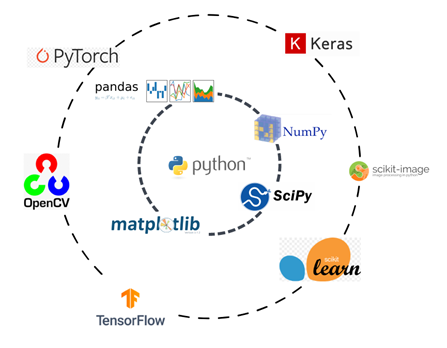
\includegraphics[width=0.5\textwidth]{Images/8.Technology_Stack/python_ecosystem.png}
    \caption{The Python Ecosystem in Machine Learning}
    \label{fig:python_ecosystem}
\end{figure}

\subsection{HTML, CSS, Javascript}
HTML (HyperText Markup Language), CSS (Cascading Style Sheets), and Javascript are the three core technologies of the web development field. 
\begin{itemize}

    \item \textbf{HTML (Hyper Text Markup Language)} is used to define the structure of a web page. Every web page consists of a set of HTML elements. Each HTML element is represented by a tag. The web browser reads the HTML tags from top to bottom and renders the web page accordingly.

    \item \textbf{CSS (Cascading Style Sheets)}: the language for defining the style of a web page. CSS is used to define the position, size, color, font, etc of the HTML elements. With the help of HTML and CSS, we can build a beautiful and responsive static web page. To make the website interactive, we need the programming language, and Javascript is the most popular choice.

    \item \textbf{JavaScript} is a scripting or programming language that allows you to implement complex features on web pages. With Javascript, we can add the dynamic behavior of the web page. For example, we can use Javascript to validate the form, change the content of the web page, handle user's input etc.
\end{itemize}

\begin{figure}[ht]
    \centering
    
\includegraphics[width=0.8\textwidth]{Images/8.Technology_Stack/html_css_js.png}
    \caption{HTML, CSS, and Javascript}
    \label{fig:html_css_javascript}
\end{figure}

\section{Libraries and Frameworks}
\subsection{Scrapy}
Scrapy is a free and open-source Python framework for web scraping. It provides a simple API for crawling the data from the web page. Scrapy is built on top of Twisted, an asynchronous networking framework. Scrapy is a powerful tool for web scraping. It can be used to automate the process of crawling data from the web page. In this project, we use Scrapy to crawl the rental data from real estate websites.
\begin{figure}[ht]
    \centering
    
\includegraphics[width=0.5\textwidth]{Images/8.Technology_Stack/scrapy.png}
    \caption{Scrapy}
    \label{fig:scrapy}
\end{figure}

\subsection{Puppeteer}
In our project, we need to crawl the data from Facebook pages. Facebook is a client-side rendered website, which means that the HTML content is generated by Javascript. A Scrapy spider cannot crawl the data from Facebook pages because it just downloads and parses the HTML content to get the data. However, with client-side rendered websites like Facebook, the HTML content does not contain the data that we need. Therefore, we need to use a tool that can execute the Javascript code to get the data. In this case, Puppeteer is a good choice. Puppeteer is a powerful tool for web scraping. The advantage of Puppeteer is that it can execute the Javascript code and get the data from the client-side rendered websites. In our project, we use Puppeteer to crawl the data from Facebook pages.

\begin{figure}[ht]
    \centering 
    \includegraphics[height=0.2\textheight]{Images/8.Technology_Stack/puppeteer.png}
\end{figure}

\subsection{React and Next.js}
\textbf{React} is the JavaScript library developed by Facebook for building user interfaces. React is a component-based library. It means that a React application is built from a set of encapsulated components. Each component is a reusable piece of code that can represent both a part of the user interface and its logic. React library helps developers to build a large and complex user interface simply. However, React is just a UI library, it missing some tools for building a complete web application such as routing, server-side rendering and state management. Therefore, when working with React, we need to use other libraries to extend its functionality. 

For these reasons, we use \textbf{NextJS} to build the web application. NextJS is a framework built on top of React, so NextJS has all the features of React and also provides some useful features such as routing and server-side rendering. Using NextJS helps us reduce the amount of time to set up the project and also takes advantage of server-side rendering to improve the performance of the web application.

\begin{figure}[ht]
    \centering
    \begin{subfigure}{0.4\textwidth}
        \centering
        \includegraphics[width=0.7\textwidth]{Images/8.Technology_Stack/react_logo.png}
        \caption{React}
    \end{subfigure}
    \begin{subfigure}{0.4\textwidth}
        \centering
        \includegraphics[width=\textwidth]{Images/8.Technology_Stack/nextjs_logo.png}
        \caption{NextJS}
    \end{subfigure}
\end{figure}

\subsection{FastAPI}
FastAPI is a modern, fast (high-performance), web framework for building APIs with Python. FastAPI is one of the most popular web frameworks for building APIs in Python. FastAPI provides some useful features such as \cite{fastapi}:
\begin{itemize}
    \item FastAPI is easy to learn and use. It has a simple and clean syntax.
    \item FastAPI is fast. It is built on top of Starlette and Pydantic, so it has high performance.
    \item Fast to code: FastAPI has a simple and intuitive API, so we can build the API quickly.
    \item Fewer bugs: Reduce about 40\% of human (developer) induced errors
\end{itemize} 

\noindent Within the scope of our project, we use FastAPI to build the API server for the AI services. 

\begin{figure}[ht]
    \centering
    \includegraphics[width=0.5\textwidth]{Images/8.Technology_Stack/fastapi_logo.png}
    \caption{FastAPI}
    \label{fig:fastapi}
\end{figure}

\subsection{MongoDB}
MongoDB is a document-oriented database. It stores the data in the form of documents. Each document is a set of key-value pairs. MongoDB is a NoSQL database, so it does not require a predefined schema. The reason for choosing MongoDB is the flexibility. Our data is crawled from different sources, so the data does not have a fixed schema. Therefore, using MongoDB helps us store the data easily.

Besides, MongoDB has a cloud version called MongoDB Atlas. MongoDB Atlas is a fully managed cloud database. It provides us with a simple way to deploy, operate, and scale the MongoDB database in the cloud. In our project, we use MongoDB Atlas to store the data.

\begin{figure}[ht]
    \centering
    \includegraphics[width=0.5\textwidth]{Images/8.Technology_Stack/mongodb_logo.png}
    \caption{MongoDB}
    \label{fig:mongodb}
\end{figure}


\subsection{Pandas}
Pandas is a Python library for data manipulation and analysis. It provides simple and powerful functions to manipulate the data. In our project, we use Pandas to preprocess the data before feeding it to the machine learning model.

\begin{figure}[ht]
    \centering
    \includegraphics[width=0.5\textwidth]{Images/8.Technology_Stack/pandas_logo.png}
    \caption{Pandas}
    \label{fig:pandas} 
\end{figure}

\subsection{Matplotlib}
Matplotlib is a comprehensive library for creating static, animated, and interactive visualizations in Python. With Matplotlib, we can create many types of charts such as line charts, bar charts, pie charts, etc. Using Matplotlib helps us visualize the data and understand the data better.

\begin{figure}[ht]
    \centering
    \includegraphics[width=0.5\textwidth]{Images/8.Technology_Stack/matplotlib_logo.png}
    \caption{Matplotlib}
    \label{fig:matplotlib}
\end{figure}

\subsection{Pytorch}
Pytorch is an open-source machine learning framework based on the Python programming language and the Torch library. It is used in many fields in machine learning such as Computer Vision and Natural language processing.  Pytorch provides some features that help us build the machine learning models easily such as:
\begin{itemize}
    \item Tensor computation with strong GPU acceleration. It helps us take advantage of GPU to speed up the training process.
    \item Automatic differentiation: As we know building the machine learning model requires the forward and backward propagation process. With Pytorch, we just need to define the forward propagation process, Pytorch will automatically compute the backward propagation process and update the parameters of the model.
    \item Pytorch provides many useful libraries for building the machine learning model and is compatible with other popular libraries such as Numpy and Pandas.
\end{itemize}

\noindent Besides these useful features, Pytorch is open-source and has a strong community. For these reasons, we choose Pytorch to build machine-learning models for the intent classifier and entity extractor.

\begin{figure}[ht]
    \centering
    \includegraphics[width=0.5\textwidth]{Images/8.Technology_Stack/pytorch_logo.png}
    \caption{Pytorch}
    \label{fig:pytorch}
\end{figure}

\subsection{Transformers}
Transformers provides APIs and tools to easily download and train state-of-the-art pre-trained models. These pre-trained models support common tasks in different modalities such as Natural Language Processing (NLP), Computer Vision (CV) and Speech Recognition (ASR). After training the model, Transformers also provides a way to share the model with the community on the Hugging Face Hub. The Hub now has more than 120k models, 20k datasets and 50k demos. This is a central place where anyone can share, explore, discover and experiment with open-source Machine Learning \cite{huggingface}.

\begin{figure}[ht]
    \centering
    \includegraphics[width=0.5\textwidth]{Images/8.Technology_Stack/huggingface_logo.png}
    \caption{Hugging Face}
    \label{fig:huggingface}
\end{figure}

\subsection{PhoBERT}
PhoBERT is the pre-trained language model for Vietnamese. PhoBERT is trained on a large corpus of Vietnamese text data with more than 20GB of Wikipedia and News text. PhoBERT is compatible with the Transformers library, so we can easily download and use the pre-trained model from the Hugging Face Hub. In our project, we use PhoBERT in our machine learning models \cite{phobert}.

\section{Tools}

\subsection{Git and GitHub}
\textbf{Git} is a distributed version control system. Using Git helps us manage the source code of the project easily. Git provides many useful features such as branching, merging, and tagging. With these features, Git allows developers to work on the same project at the same time without worrying about conflicts. Git is also a cross-platform tool, so we can use it on many operating systems such as Windows, Linux, and macOS.

\begin{figure}[ht]
    \centering
    \includegraphics[width=0.5\textwidth]{Images/8.Technology_Stack/git_logo.png}
    \caption{Git}
    \label{fig:git}
\end{figure}

\noindent \textbf{GitHub} is a platform for hosting and collaborating on Git repositories. GitHub allows developers to store the source code on the cloud and collaborate with other developers.

\begin{figure}
    \centering
    \includegraphics[width=0.5\textwidth]{Images/8.Technology_Stack/github_logo.png}
    \caption{GitHub}
    \label{fig:github}
\end{figure}

\subsection{Github Actions}
GitHub actions is a CI/CD tool provided by GitHub. It helps us automate the process of building, testing, and deploying the application. With GitHub actions, we can easily set up the CI/CD pipeline for the project. In our project, we use GitHub actions to build and deploy the web application to the server.

\subsection{Dagshub}
With GitHub, developers can only manage their source code. But in the machine learning project, we also need to manage the data and the model. So \textbf{Dagshub} appears to solve this problem.
Dagshub is a platform for developers to manage their machine-learning projects. Dagshub is built on top of Git, so it has all the features of Git. Besides, Dagshub also provides some useful features for managing the data and the model.

\begin{figure}[ht]
    \centering
    \includegraphics[width=0.5\textwidth]{Images/8.Technology_Stack/dagshub_logo.png}
    \caption{Dagshub}
    \label{fig:dagshub}
\end{figure}


% \chapter{Implementation}
\chapter{Implementation}
In this chapter, we present the process of implementing the system. Up to the end of the Specialized Project, we have completed the following tasks:
\begin{itemize}
    \item Designed a mockup interface for the website.
    \item Developed a crawler to collect data from both real estate websites and Facebook groups.
    \item Developed an intent classification model to classify the user's intent based on the user's message.
\end{itemize}

\section{Mockup interface}
We have implemented the mockup interface in Figma for the Tenant Landing Page, Search page, Rental detail page and Chatbot interface. All of the mockup interfaces are in \href{https://www.figma.com/proto/4W6eMgIgZQaSfi5h8Mn8Af/Material-UI-for-Figma-(and-MUI-X)-(Community)-(Copy)?page-id=4230%3A722&type=design&node-id=6609-8548&viewport=4481%2C1065%2C1&t=QoVk3s8CM7w3qcvh-1&scaling=scale-down-width&starting-point-node-id=6759%3A76810}{here}

\subsection{Tenant pages}
We have a tenant landing page that allows the user to view the list of rental posts in the system. You can see the design in Figure \ref{fig:tenant-landing-page}

\clearpage
\begin{figure}[ht]
    \centering
    \includegraphics[width=0.8\textwidth]{Images/Mockup/landing_page.png}
    \caption{The tenant landing page}
    \label{fig:tenant-landing-page}
\end{figure}

The list of rental posts is displayed in the form of a card, see Figure \ref{fig:rental-posts}

\begin{figure}[ht]
    \centering
    \includegraphics[width=0.8\textwidth]{Images/Mockup/rental_posts.png}
    \caption{The list of rental posts}
    \label{fig:rental-posts} 
\end{figure}

When the user clicks on a rental post, the rental detail page will be displayed. The rental detail page contains the information of the rental post such as the name, address, price, area, description, owner name, owner contact, post date, and the link to the original post. The rental detail page is shown in Figures \ref{fig:rental-detail-page} and \ref{fig:rental-detail-page-2}

\begin{figure}[ht]
    \centering
    \includegraphics[width=\textwidth]{Images/Mockup/rental_detail_1.png}
    \caption{The rental detail page}
    \label{fig:rental-detail-page}
\end{figure}

\begin{figure}[ht]
    \centering
    \includegraphics[width=\textwidth]{Images/Mockup/rental_detail_2.png}
    \caption{The rental detail page (continue)}
    \label{fig:rental-detail-page-2}
\end{figure}
\clearpage

\subsection{Search and Filter page}
Our website allows the user to search by keyword and filter the rental posts by some criteria such as property type, price range, number of rooms, number of beds, area and amenities. 

\begin{figure}[ht]
    \centering
    \includegraphics[width=\textwidth]{Images/Mockup/rental_filter_1.png}
    \caption{The rental filter page}
    \label{fig:rental-filter-1} 
\end{figure}

\begin{figure}[ht]
    \centering
    \includegraphics[width=\textwidth]{Images/Mockup/rental_filter_2.png}
    \caption{The rental filter page (continue)}
    \label{fig:rental-filter-2} 
\end{figure}

\begin{figure}[ht]
    \centering
    \includegraphics[width=\textwidth]{Images/Mockup/rental_filter_3.png}
    \caption{The rental filter page (continue)}
    \label{fig:rental-filter-3} 
\end{figure}

\clearpage

\subsection{Chatbot interface}

\begin{figure}[ht]
    \centering
    \includegraphics[width=\textwidth]{Images/Mockup/chatbot.png}
    \caption{The chatbot interface}
    \label{fig:chatbot}
\end{figure}

\clearpage

\subsection{Landlord pages}
We have landlord pages that allow the landlord to post their rental information and manage their property. Figures \ref{fig:create-rental-1} and \ref{fig:create-rental-2} show the form for the landlord to create a new rental post

\begin{figure}[ht]
    \centering
    \includegraphics[width=0.8\textwidth]{Images/Mockup/create_rental_1.png}
    \caption{The form for the landlord to create a new rental post}
    \label{fig:create-rental-1}
\end{figure}

\begin{figure}[ht]
    \centering
    \includegraphics[width=0.8\textwidth]{Images/Mockup/create_rental_2.png}
    \caption{The form for the landlord to create a new rental post (continue)}
    \label{fig:create-rental-2}
\end{figure}

\clearpage

\begin{figure}[ht]
    \centering
    \includegraphics[width=0.8\textwidth]{Images/Mockup/property_list.png}
    \caption{The list of Landlords' properties}
    \label{fig:property_list}
\end{figure}

\begin{figure}[ht]
    \centering
    \includegraphics[width=0.8\textwidth]{Images/Mockup/update_rental.png}
    \caption{The form for the landlord to update a rental post}
    \label{fig:update_rental}
\end{figure}

\clearpage

\section{Crawler service}

\subsection{The Facebook Crawler}
We developed a tool that receives the list of Facebook pages and group URLs as input. Then this tool will get all the posts from these pages and groups and store them in the output file. The tool is implemented using NodeJS and the Puppeteer library.

We chose the list of 40 Facebook pages and groups in the real estate domain, especially the ones that have the most interactions. The list of these pages and groups is stored in the input file. The sample of the input file is shown in Figure \ref{fig:facebook-crawler-input}.

\begin{figure}[ht]
    \centering
    \includegraphics[width=0.8\textwidth]{Images/9.Implementation/facebook_crawler_input.png}
    \caption{The sample input of the Facebook crawler}
    \label{fig:facebook-crawler-input}
\end{figure}

When running the tool, the tool will read the input file and get the list of Facebook pages and groups. Then it will open a new browser window and log in to Facebook. After that, it will visit each page and group in the list and get all the posts from these pages and groups. Finally, it will store the posts in the output file. The output file is a text file that contains the list of posts in text format. Each post is separated by a new line character. After the tool finishes crawling all the posts, we get the output file that contains nearly \textbf{2000 posts}. The sample output of the tool is shown in Figure \ref{fig:facebook-crawler}.

\begin{figure}[ht]
    \centering
    \includegraphics[width=0.8\textwidth]{Images/9.Implementation/facebook_crawler_output.png}
    \caption{The sample output of the Facebook crawler}
    \label{fig:facebook-crawler}
\end{figure}

\subsection{The Real Estate Website Crawler}
We also developed a tool that crawls the data from some popular real estate websites in Vietnam such as mogi.vn. The tool is implemented using Python and Scrapy. Because these websites are server-side rendered websites, we can take advantage of the Scrapy library to crawl the data. 

From the website link, we developed a Spider Scrapy. The main role of the Spider is downloading the content of the website parsing the content and getting the data by using CSS selector. The sample code of the parser is shown below

\begin{lstlisting}[language=Python]
def parse_detail_info(self, response):
    general_info = response.css('div.main-info')
    main_info = response.css('div.info-attrs.clearfix > *')
    agent_name_link = response.css('div.agent-name::text').get()
    agent_name_no_link = response.css('div.agent-name a::text').get()
    agent_name = agent_name_link if agent_name_link else agent_name_no_link

    yield rental_item = {
        'name': general_info.css('div.title h1::text').get(),
        'address': general_info.css('div.address::text').get(),
        'price': general_info.css('div.price::text').get(),
        'area': main_info[0].css('span:nth-of-type(2)::text').get(),
        'description': response.css('div.info-content-body').get(),
        'owner_name': agent_name,
        'owner_contact': response.css('div.agent-contact').get(),
        'post_date': main_info[2].css('span:nth-of-type(2)::text').get(),
        'prop_info_url': response.meta.get('prop_info_url')
    }
\end{lstlisting}

After crawling, we got the data in CSV format with \textbf{12288 rows}. Each row is a rental post with the following fields: name, address, price, area, description, owner name, owner contact, post date, and the link to the original post. Figure \ref{fig:sample-crawling-data} shows the sample data returned by the crawler. 

\begin{figure}[ht]
    \centering
    \includegraphics[width=0.8\textwidth]{Images/9.Implementation/sample_crawling_data.png}
    \caption{The sample data returned by the crawler}
    \label{fig:sample-crawling-data}
\end{figure}

The full dataset can be found \href{https://www.kaggle.com/datasets/ef8770394a7256fd4e5270fd4a3692235a620fc85ac18128efd1b44d31aa5b1b}{here}.

\section{Intent classification model}
We have implemented the intent classification model as discussed section in \ref{sec:intent-classification-model} with Pytorch and PhoBERT library. The model is trained on the dataset containing 1000 labeled messages. We split the dataset into 2 parts: 80\% for training and 20\% for testing. We trained the model for 10 epochs with a batch size of 32. Figure \ref{fig:intent-classification-result} shows the accuracy of the model during the training process. Overall, the model achieves an accuracy of 97.4\% on the training set and 96.5\% on the test set. 

\begin{figure}[ht]
    \centering
    \includegraphics[width=0.7\textwidth]{Images/9.Implementation/intent_classifier_accuracy.png} 
    \caption{The accuracy of the intent classification model during the training process}
    \label{fig:intent-classification-accuracy}
\end{figure}

\begin{figure}[ht]
    \centering
    \includegraphics[width=0.8\textwidth]{Images/9.Implementation/intent_classifier_result.png}
    \caption{The sample result of intent classification model}
    \label{fig:intent-classification-result}
\end{figure}

% \chapter{Result and Evalutaion}

\chapter{Conclusion}
In this chapter, we will have a summary of the progress for the first phase, and then discuss some plans for the next phase of the project.

\section{Summary}
In this first phase of the thesis, the goal is to learn and prepare the knowledge that is needed for the implementation of the project, specify the problem and the scope of the project as well as design the system architecture. To be more specific, we have done building the system architecture, learning the background knowledge, doing some research on the related works and developing the data crawler service and the intent classifier.

\subsection{Challenges}
Throughout the process of doing this project, we have faced some challenges:

\begin{itemize}
    \item The first thing and also the biggest challenge is the process of learning background knowledge. Both of us do not have much experience working in the field of Machine Learning and Natural Language Processing. But it is also an opportunity for us to learn new things. 

    \item The next challenge is in the process of crawling data from the internet. Some website has a lot of security measures to prevent the crawler from crawling the data. Therefore, we have to find a way to bypass these security measures.

    \item The last challenge is in the data processing. We have a lot of data, but to use the data for training the NER model, we have to annotate the data first. The process of annotating data is very time-consuming and requires a lot of effort.
\end{itemize}

\subsection{Experience}
\begin{itemize}
    \item Research and paper reading skill
    \item Time management for a big project
    \item Communication, task assignment between members
    \item Self-motivate and self-discipline
    \item NLP project experience
    \item Data crawling project experience
\end{itemize}

\section{Future Plan}
Regarding the plan for the next phase, there are still many main tasks that must be completed:

\begin{itemize}
    \item Prepare the dataset for training the NER model.
    \item Finish creating a Machine Reading Comprehension dataset and an Intent/Entity dataset.
    \item Implement the user interface for the website and chatbot.
    \item Implement the database and the back-end server.
    \item Testing and Evaluation
\end{itemize}
\renewcommand{\bibname}{References}

\printbibliography
\appendix
% \chapter{Workload of Members}
\section{Members Workload}
\begin{center}
\begin{tabular}{|c|c|c|p{5cm}|}
\hline
\textbf{No.} & \textbf{Fullname} & \textbf{Student ID} & \textbf{Workload} \\
\hline 
1. & Luu Chan Hung & 1952063 & Machine-learning related research and implementation. \\
&  &  & Back-end development. \\
& & & Manage data preparation group.\\
\hline 
2. & Nguyen Thanh Hung & 1952272 & Front-end development. \\
&  &  & Back-end development. \\
& & & Manage data preparation group.\\
\hline 
\end{tabular}
\end{center}
% \chapter{First Approach for System Architecture}

\begin{figure}[h]
\begin{center}
\includegraphics[scale = 0.3]{Images/mono_design.png}
\end{center}
\caption{Monolithic architecture design}
\end{figure}
In this approach, every module is packed into a tightly-coupled system. As the user message can be received in the form of text or voice, there are two ways to process input. If it is text-based, it will be transferred directly into a Natural Language Understanding module, which will classify the intents and entities of the sentence. On the other hand, voice-based will be processed by a Speech-to-Text module before into NLU. A Conversation Manager is in control of managing the flow of the conversation. Moreover, if the intent is a functional intent, an Answer Generator is used to find the answer. Lastly, a Machine Learning Pipeline module is used for creating an automated training pipeline.

The idea behind a Monolithic approach is straightforward. Since our system can be divided into 3 big modules: A Chatbot, A Machine Reading Comprehension module, and an MLOps module, this approach provides a clear and comprehensive view at a component level. Furthermore, compared to the next approach, it is better to keep the first approach for the purpose of better understanding the system. However, a Monolithic architecture has some big challenges for our system:
\begin{itemize}
    \item With this design, it also means that we will have many separate Machine Learning models (1 for the Intent classifier, 1 for Named Entity Recognizer, 1 for MRC), and 2 Retrievers (1 for FAQ and 1 for Document). As a result, the system is expensive and inefficient.
    \item It also suffers a scalability problem. With this many models, running the whole system is a problem. Therefore, it is almost impossible to scale this system.
    \item Due to its tightly-coupled nature, it is also difficult to integrate a CI/CD and CT pipeline. As the whole system must be loaded all at once, if we want to deploy a new model, it must restart the system.
\end{itemize}


\chapter{Data preparation team}
\begin{table}[ht]
    \centering
    \begin{tabular}{|l|c|}
        \hline
         \textbf{Full name} & \textbf{Student ID} \\
         \hline
         Phạm Văn Tâm & 2151254\\
         \hline
         Đỗ Nhật Quang & 2151246 \\
         \hline
         Lại Huy Anh & 2110725\\
         \hline
         Nguyễn Lê Hữu Quang & 2151247 \\
         \hline
         Nguyễn Hồ Phúc Nguyên & 2151236 \\
         \hline
         Lương Kim Long & 2151112 \\
         \hline
         Cao Minh Tuấn & 2151159 \\
         \hline
         Trần Hồng Lam & 2151218\\
         \hline
         Chu Thanh Đồng & 2151065 \\
         \hline
         Nguyễn Nam Vũ & 2151278 \\
         \hline
         Trần Trung Hiếu Nam & 2151122 \\
         \hline
         Trần Quang Nguyên Ánh & 2151047 \\
         \hline
         Lâm Hoàng Nhật & 2151238 \\
         \hline
         Đào Vũ Minh Trí & 2151153 \\
         \hline
         Lê Anh Tuấn & 2110643 \\
         \hline
         Nguyễn Hữu Đức & 2151189 \\
         \hline
         Trần Thị Minh Tâm & 2151032 \\
         \hline
         Nguyễn Giao Gia Bảo & 2110791 \\
         \hline
         Ngô Tiến Dũng & 2151185 \\
         \hline
         Vũ Huy Bảo & 2151177 \\
         \hline
         Đồng Trinh Hoàng Nguyên & 2151124 \\
         \hline
         Võ Hoàng Phúc & 2151029 \\
         \hline
         Văn Thiên Lâm & 2151110 \\
         \hline
         Nguyễn Gia Huy & 2151016 \\
         \hline
         Nguyễn Huy Hoàng & 2151197 \\
         \hline
         Phạm Minh Đạt & 2151007 \\
         \hline
         Phạm Gia Khang & 2151209 \\
         \hline
         Nguyễn Thái Bình Dương & 2051103 \\
         \hline
         Lâm Ngọc Cầm & 2151281 \\
         \hline
         Phạm Khắc Thanh Tùng & 2151274 \\
         \hline
         Nguyễn Thế Khang Hi & 2151070 \\
         \hline
         Võ Phú Thành & 2151259 \\
         \hline
         Huỳnh Lê Phi Long & 2151111 \\
         \hline
         Phạm Bình Dương & 2151283 \\
         \hline
         Nguyễn Xuân Khoa & 2051137 \\
         \hline
         Ngô Đình Anh Khoa & 2151212 \\
         \hline
         Trần Duy Trung Hiếu & 2151193 \\
         \hline
         Trần Quang Minh & 2151230 \\
         \hline
    \end{tabular}
    \caption{Data preparation team}
    \label{tab:my_label}
\end{table}

\end{document}
